%&preformat-disser
\RequirePackage[l2tabu,orthodox]{nag} % Раскомментировав, можно в логе получать рекомендации относительно правильного использования пакетов и предупреждения об устаревших и нерекомендуемых пакетах
% Формат А4, 14pt (ГОСТ Р 7.0.11-2011, 5.3.6)
\documentclass[a4paper,14pt,oneside,openany]{memoir}

%%%%%%%%%%%%%%%%%%%%%%%%%%%%%%%%%%%%%%%%%%%%%%%%%%%%%%%%%%%%%%%%%%%%%%%%%%%%%%%%
%%%% Файл упрощённых настроек шаблона, общих для диссертации и автореферата %%%%
%%%%%%%%%%%%%%%%%%%%%%%%%%%%%%%%%%%%%%%%%%%%%%%%%%%%%%%%%%%%%%%%%%%%%%%%%%%%%%%%

%%% Режим черновика %%%
\makeatletter
\@ifundefined{c@draft}{
  \newcounter{draft}
  \setcounter{draft}{0}  % 0 --- чистовик (максимальное соблюдение ГОСТ)
                         % 1 --- черновик (отклонения от ГОСТ, но быстрая
                         %       сборка итоговых PDF)
}{}
\makeatother

%%% Пометки в тексте %%%
\makeatletter
\@ifundefined{c@showmarkup}{
  \newcounter{showmarkup}
  \setcounter{showmarkup}{0}  % 0 --- скрыть пометки
                              % 1 --- показывать пометки
}{}
\makeatother

%%% Использование в pdflatex шрифтов не по-умолчанию %%%
\makeatletter
\@ifundefined{c@usealtfont}{
  \newcounter{usealtfont}
  \setcounter{usealtfont}{1}    % 0 --- шрифты на базе Computer Modern
                                % 1 --- использовать пакет pscyr, при его
                                %       наличии
                                % 2 --- использовать пакет XCharter, при наличии
                                %       подходящей версии
}{}
\makeatother

%%% Использование в xelatex и lualatex семейств шрифтов %%%
\makeatletter
\@ifundefined{c@fontfamily}{
  \newcounter{fontfamily}
  \setcounter{fontfamily}{2}  % 0 --- CMU семейство. Используется как fallback;
                              % 1 --- Шрифты от MS (Times New Roman и компания)
                              % 2 --- Семейство Liberation
}{}
\makeatother

%%% Библиография %%%
\makeatletter
\@ifundefined{c@bibliosel}{
  \newcounter{bibliosel}
  \setcounter{bibliosel}{1}   % 0 --- встроенная реализация с загрузкой файла
                              %       через движок bibtex8;
                              % 1 --- реализация пакетом biblatex через движок
                              %       biber
}{}
\makeatother

%%% Вывод типов ссылок в библиографии %%%
\makeatletter
\@ifundefined{c@mediadisplay}{
  \newcounter{mediadisplay}
  \setcounter{mediadisplay}{1}   % 0 --- не делать ничего; надписи [Текст] и
                                 %       [Эл. ресурс] будут выводиться только в ссылках с
                                 %       заполненным полем `media`;
                                 % 1 --- автоматически добавлять надпись [Текст] к ссылкам с
                                 %       незаполненным полем `media`; таким образом, у всех
                                 %       источников будет указан тип, что соответствует
                                 %       требованиям ГОСТ
                                 % 2 --- автоматически удалять надписи [Текст], [Эл. Ресурс] и др.;
                                 %       не соответствует ГОСТ
                                 % 3 --- автоматически удалять надпись [Текст];
                                 %       не соответствует ГОСТ
                                 % 4 --- автоматически удалять надпись [Эл. Ресурс];
                                 %       не соответствует ГОСТ
}{}
\makeatother

%%% Предкомпиляция tikz рисунков для ускорения работы %%%
\makeatletter
\@ifundefined{c@imgprecompile}{
  \newcounter{imgprecompile}
  \setcounter{imgprecompile}{0}   % 0 --- без предкомпиляции;
                                  % 1 --- пользоваться предварительно
                                  %       скомпилированными pdf вместо генерации
                                  %       заново из tikz
}{}
\makeatother
            % общие настройки шаблона
%%% Проверка используемого TeX-движка %%%
\newif\ifxetexorluatex   % определяем новый условный оператор (http://tex.stackexchange.com/a/47579)
\ifxetex
    \xetexorluatextrue
\else
    \ifluatex
        \xetexorluatextrue
    \else
        \xetexorluatexfalse
    \fi
\fi

\newif\ifsynopsis           % Условие, проверяющее, что документ --- автореферат

\usepackage{etoolbox}[2015/08/02]   % Для продвинутой проверки разных условий
\providebool{presentation}

\usepackage{comment}    % Позволяет убирать блоки текста (добавляет
                        % окружение comment и команду \excludecomment)

%%% Поля и разметка страницы %%%
\usepackage{pdflscape}  % Для включения альбомных страниц
\usepackage{geometry}   % Для последующего задания полей

%%% Математические пакеты %%%
\usepackage{amsthm,amsmath,amscd}   % Математические дополнения от AMS
\usepackage{amsfonts,amssymb}       % Математические дополнения от AMS
\usepackage{mathtools}              % Добавляет окружение multlined
\usepackage{xfrac}                  % Красивые дроби
\usepackage[
    locale = DE,
    list-separator       = {;\,},
    list-final-separator = {;\,},
    list-pair-separator  = {;\,},
    list-units           = single,
    range-units          = single,
    range-phrase={\text{\ensuremath{-}}},
    % quotient-mode        = fraction, % красивые дроби могут не соответствовать ГОСТ
    fraction-function    = \sfrac,
    separate-uncertainty,
    ]{siunitx}[=v2]                 % Размерности SI
\sisetup{inter-unit-product = \ensuremath{{}\cdot{}}}

% Кириллица в нумерации subequations
% Для правильной работы требуется выполнение сразу после загрузки пакетов
\patchcmd{\subequations}{\def\theequation{\theparentequation\alph{equation}}}
{\def\theequation{\theparentequation\asbuk{equation}}}
{\typeout{subequations patched}}{\typeout{subequations not patched}}

%%%% Установки для размера шрифта 14 pt %%%%
%% Формирование переменных и констант для сравнения (один раз для всех подключаемых файлов)%%
%% должно располагаться до вызова пакета fontspec или polyglossia, потому что они сбивают его работу
\newlength{\curtextsize}
\newlength{\bigtextsize}
\setlength{\bigtextsize}{13.9pt}

\makeatletter
%\show\f@size    % неплохо для отслеживания, но вызывает стопорение процесса,
                 % если документ компилируется без команды  -interaction=nonstopmode
\setlength{\curtextsize}{\f@size pt}
\makeatother

%%% Кодировки и шрифты %%%
\ifxetexorluatex
    \ifpresentation
        \providecommand*\autodot{} % quick fix for polyglossia 1.50
    \fi
    \PassOptionsToPackage{no-math}{fontspec}    % https://tex.stackexchange.com/a/26295/104425
    \usepackage{polyglossia}[2014/05/21]        % Поддержка многоязычности
                                        % (fontspec подгружается автоматически)
\else
   %%% Решение проблемы копирования текста в буфер кракозябрами
    \ifnumequal{\value{usealtfont}}{0}{}{
        \input glyphtounicode.tex
        \input glyphtounicode-cmr.tex %from pdfx package
        \pdfgentounicode=1
    }
    \usepackage{cmap}   % Улучшенный поиск русских слов в полученном pdf-файле
    \ifnumequal{\value{usealtfont}}{2}{}{
        \defaulthyphenchar=127  % Если стоит до fontenc, то переносы
                                % не впишутся в выделяемый текст при
                                % копировании его в буфер обмена
    }
    \usepackage{textcomp}
    \usepackage[T1,T2A]{fontenc}                    % Поддержка русских букв
    \ifnumequal{\value{usealtfont}}{1}{% Используется pscyr, при наличии
        \IfFileExists{pscyr.sty}{\usepackage{pscyr}}{}  % Подключение pscyr
    }{}
    \usepackage[utf8]{inputenc}[2014/04/30]         % Кодировка utf8
    \usepackage[english, russian]{babel}[2014/03/24]% Языки: русский, английский
    \makeatletter\AtBeginDocument{\let\@elt\relax}\makeatother % babel 3.40 fix
    \ifnumequal{\value{usealtfont}}{2}{
        % http://dxdy.ru/post1238763.html#p1238763
        \usepackage[scaled=0.914]{XCharter}[2017/12/19] % Подключение русифицированных шрифтов XCharter
        \usepackage[charter, vvarbb, scaled=1.048]{newtxmath}[2017/12/14]
        \ifpresentation
        \else
            \setDisplayskipStretch{-0.078}
        \fi
    }{}
\fi

%%% Оформление абзацев %%%
\ifpresentation
\else
    \indentafterchapter     % Красная строка после заголовков типа chapter
    \usepackage{indentfirst}
\fi

%%% Цвета %%%
\ifpresentation
\else
    \usepackage[dvipsnames, table, hyperref]{xcolor} % Совместимо с tikz
\fi

%%% Таблицы %%%
\usepackage{longtable} % Длинные таблицы
\usepackage{multirow,makecell}   % Улучшенное форматирование таблиц
\usepackage{tabulary,tabularray} % Таблицы с автоматически подбирающейся
                                 % шириной столбцов
\UseTblrLibrary{booktabs}
\ExplSyntaxOn% define \IfTokenListEmpty to use \captionof with tabularray
\prg_generate_conditional_variant:Nnn \tl_if_empty:n { e } { TF }
\let \IfTokenListEmpty = \tl_if_empty:eTF
\ExplSyntaxOff

\usepackage{threeparttable}      % автоматический подгон ширины подписи таблицы

%%% Общее форматирование
%\usepackage{soul}% Поддержка переносоустойчивых подчёркиваний и зачёркиваний
\usepackage{icomma}  % Запятая в десятичных дробях

%%% Оптимизация расстановки переносов и длины последней строки абзаца
\IfFileExists{impnattypo.sty}{% проверка установленности пакета impnattypo
    \ifluatex
        \ifnumequal{\value{draft}}{1}{% Черновик
            \usepackage[hyphenation, lastparline, nosingleletter, homeoarchy,
            rivers, draft]{impnattypo}
        }{% Чистовик
            \usepackage[hyphenation, lastparline, nosingleletter]{impnattypo}
        }
    \else
        \usepackage[hyphenation, lastparline]{impnattypo}
    \fi
}{}

%% Векторная графика

\usepackage{tikz}                   % Продвинутый пакет векторной графики
\usetikzlibrary{chains}             % Для примера tikz рисунка
\usetikzlibrary{shapes.geometric}   % Для примера tikz рисунка
\usetikzlibrary{shapes.symbols}     % Для примера tikz рисунка
\usetikzlibrary{arrows}             % Для примера tikz рисунка

\usepackage[european,cuteinductors]{circuitikz} % Электрические схемы
\usepackage{pgfplots}                           % Графики
\pgfplotsset{compat=newest}
\usepgfplotslibrary{groupplots,units}
\pgfkeys{/pgf/number format/.cd,use comma,1000 sep={}} % форматирование чисел в графиках

%%% Гиперссылки %%%
\ifxetexorluatex
    \let\CYRDZE\relax
\fi
\usepackage{hyperref}[2012/11/06]

%%% Изображения %%%
\usepackage{graphicx}[2014/04/25]   % Подключаем пакет работы с графикой
\usepackage{caption}                % Подписи рисунков и таблиц
\usepackage{subcaption}             % Подписи подрисунков и подтаблиц
\usepackage{pdfpages}               % Добавление внешних pdf файлов

%%% Счётчики %%%
\usepackage{aliascnt}
\usepackage[figure,table]{totalcount}   % Счётчик рисунков и таблиц
\usepackage{totcount}   % Пакет создания счётчиков на основе последнего номера
                        % подсчитываемого элемента (может требовать дважды
                        % компилировать документ)
\usepackage{totpages}   % Счётчик страниц, совместимый с hyperref (ссылается
                        % на номер последней страницы). Желательно ставить
                        % последним пакетом в преамбуле

%%% Продвинутое управление групповыми ссылками (пока только формулами) %%%
\ifpresentation
\else
    \usepackage[russian]{cleveref} % cleveref имеет сложности со считыванием
    % языка из babel. Такое решение русификации вывода выбрано вместо
    % определения в documentclass из опасности что-то лишнее передать во все
    % остальные пакеты, включая библиографию.

    % Добавление возможности использования пробелов в \labelcref
    % https://tex.stackexchange.com/a/340502/104425
    \usepackage{kvsetkeys}
    \makeatletter
    \let\org@@cref\@cref
    \renewcommand*{\@cref}[2]{%
        \edef\process@me{%
            \noexpand\org@@cref{#1}{\zap@space#2 \@empty}%
        }\process@me
    }
    \makeatother
\fi

\usepackage{placeins} % для \FloatBarrier

\ifnumequal{\value{draft}}{1}{% Черновик
    \usepackage[firstpage]{draftwatermark}
    \SetWatermarkText{DRAFT}
    \SetWatermarkFontSize{14pt}
    \SetWatermarkScale{15}
    \SetWatermarkAngle{45}
}{}

%%% Цитата, не приводимая в автореферате:
% возможно, актуальна только для biblatex
%\newcommand{\citeinsynopsis}[1]{\ifsynopsis\else ~\cite{#1} \fi}

% если текущий процесс запущен библиотекой tikz-external, то прекомпиляция должна быть включена
\ifdefined\tikzexternalrealjob
    \setcounter{imgprecompile}{1}
\fi

\ifnumequal{\value{imgprecompile}}{1}{% Только если у нас включена предкомпиляция
    \usetikzlibrary{external}   % подключение возможности предкомпиляции
    \tikzexternalize[prefix=images/cache/,optimize command away=\includepdf] % activate! % здесь можно указать отдельную папку для скомпилированных файлов
    \ifxetex
        \tikzset{external/up to date check={diff}}
    \fi
}{}
         % Пакеты общие для диссертации и автореферата
\synopsisfalse                      % Этот документ --- не автореферат
%%% Прикладные пакеты %%%
%\usepackage{calc}               % Пакет для расчётов параметров, например длины

%%% Для добавления Стр. над номерами страниц в оглавлении
%%% http://tex.stackexchange.com/a/306950
\usepackage{afterpage}

%%% Списки %%%
\usepackage{enumitem}

%%% Оформление списка обозначений
\usepackage[intoc]{nomencl}
\makenomenclature
\setlength{\nomitemsep}{-.8\parsep}
    % Пакеты для диссертации
% Листинги с исходным кодом программ
\usepackage{fancyvrb}
\usepackage{listings}
\lccode`\~=0\relax %Без этого хака из-за особенностей пакета listings перестают работать конструкции с \MakeLowercase и т. п. в (xe|lua)latex

% Русская традиция начертания греческих букв
\usepackage{upgreek} % прямые греческие ради русской традиции

%%% Микротипографика
%\ifnumequal{\value{draft}}{0}{% Только если у нас режим чистовика
%    \usepackage[final, babel, shrink=45]{microtype}[2016/05/14] % улучшает представление букв и слов в строках, может помочь при наличии отдельно висящих слов
%}{}

% Отметка о версии черновика на каждой странице
% Чтобы работало надо в своей локальной копии по инструкции
% https://www.ctan.org/pkg/gitinfo2 создать небходимые файлы в папке
% ./git/hooks
% If you’re familiar with tweaking git, you can probably work it out for
% yourself. If not, I suggest you follow these steps:
% 1. First, you need a git repository and working tree. For this example,
% let’s suppose that the root of the working tree is in ~/compsci
% 2. Copy the file post-xxx-sample.txt (which is in the same folder of
% your TEX distribution as this pdf) into the git hooks directory in your
% working copy. In our example case, you should end up with a file called
% ~/compsci/.git/hooks/post-checkout
% 3. If you’re using a unix-like system, don’t forget to make the file executable.
% Just how you do this is outside the scope of this manual, but one
% possible way is with commands such as this:
% chmod g+x post-checkout.
% 4. Test your setup with “git checkout master” (or another suitable branch
% name). This should generate copies of gitHeadInfo.gin in the directories
% you intended.
% 5. Now make two more copies of this file in the same directory (hooks),
% calling them post-commit and post-merge, and you’re done. As before,
% users of unix-like systems should ensure these files are marked as
% executable.
\ifnumequal{\value{draft}}{1}{% Черновик
   \IfFileExists{.git/gitHeadInfo.gin}{
      \usepackage[mark,pcount]{gitinfo2}
      \renewcommand{\gitMark}{rev.\gitAbbrevHash\quad\gitCommitterEmail\quad\gitAuthorIsoDate}
      \renewcommand{\gitMarkFormat}{\rmfamily\color{Gray}\small\bfseries}
   }{}
}{}
   % Пакеты для специфических пользовательских задач

%%%%%%%%%%%%%%%%%%%%%%%%%%%%%%%%%%%%%%%%%%%%%%%%%%%%%%%%%%%%%%%%%%%%%%%%%%%%%%%%
%%%% Файл упрощённых настроек шаблона, общих для диссертации и автореферата %%%%
%%%%%%%%%%%%%%%%%%%%%%%%%%%%%%%%%%%%%%%%%%%%%%%%%%%%%%%%%%%%%%%%%%%%%%%%%%%%%%%%

%%% Режим черновика %%%
\makeatletter
\@ifundefined{c@draft}{
  \newcounter{draft}
  \setcounter{draft}{0}  % 0 --- чистовик (максимальное соблюдение ГОСТ)
                         % 1 --- черновик (отклонения от ГОСТ, но быстрая
                         %       сборка итоговых PDF)
}{}
\makeatother

%%% Пометки в тексте %%%
\makeatletter
\@ifundefined{c@showmarkup}{
  \newcounter{showmarkup}
  \setcounter{showmarkup}{0}  % 0 --- скрыть пометки
                              % 1 --- показывать пометки
}{}
\makeatother

%%% Использование в pdflatex шрифтов не по-умолчанию %%%
\makeatletter
\@ifundefined{c@usealtfont}{
  \newcounter{usealtfont}
  \setcounter{usealtfont}{1}    % 0 --- шрифты на базе Computer Modern
                                % 1 --- использовать пакет pscyr, при его
                                %       наличии
                                % 2 --- использовать пакет XCharter, при наличии
                                %       подходящей версии
}{}
\makeatother

%%% Использование в xelatex и lualatex семейств шрифтов %%%
\makeatletter
\@ifundefined{c@fontfamily}{
  \newcounter{fontfamily}
  \setcounter{fontfamily}{2}  % 0 --- CMU семейство. Используется как fallback;
                              % 1 --- Шрифты от MS (Times New Roman и компания)
                              % 2 --- Семейство Liberation
}{}
\makeatother

%%% Библиография %%%
\makeatletter
\@ifundefined{c@bibliosel}{
  \newcounter{bibliosel}
  \setcounter{bibliosel}{1}   % 0 --- встроенная реализация с загрузкой файла
                              %       через движок bibtex8;
                              % 1 --- реализация пакетом biblatex через движок
                              %       biber
}{}
\makeatother

%%% Вывод типов ссылок в библиографии %%%
\makeatletter
\@ifundefined{c@mediadisplay}{
  \newcounter{mediadisplay}
  \setcounter{mediadisplay}{1}   % 0 --- не делать ничего; надписи [Текст] и
                                 %       [Эл. ресурс] будут выводиться только в ссылках с
                                 %       заполненным полем `media`;
                                 % 1 --- автоматически добавлять надпись [Текст] к ссылкам с
                                 %       незаполненным полем `media`; таким образом, у всех
                                 %       источников будет указан тип, что соответствует
                                 %       требованиям ГОСТ
                                 % 2 --- автоматически удалять надписи [Текст], [Эл. Ресурс] и др.;
                                 %       не соответствует ГОСТ
                                 % 3 --- автоматически удалять надпись [Текст];
                                 %       не соответствует ГОСТ
                                 % 4 --- автоматически удалять надпись [Эл. Ресурс];
                                 %       не соответствует ГОСТ
}{}
\makeatother

%%% Предкомпиляция tikz рисунков для ускорения работы %%%
\makeatletter
\@ifundefined{c@imgprecompile}{
  \newcounter{imgprecompile}
  \setcounter{imgprecompile}{0}   % 0 --- без предкомпиляции;
                                  % 1 --- пользоваться предварительно
                                  %       скомпилированными pdf вместо генерации
                                  %       заново из tikz
}{}
\makeatother
      % Упрощённые настройки шаблона

% Новые переменные, которые могут использоваться во всём проекте
% ГОСТ 7.0.11-2011
% 9.2 Оформление текста автореферата диссертации
% 9.2.1 Общая характеристика работы включает в себя следующие основные структурные
% элементы:
% актуальность темы исследования;
\newcommand{\actualityTXT}{Актуальность темы.}
% степень ее разработанности;
\newcommand{\progressTXT}{Степень разработанности темы.}
% цели и задачи;
\newcommand{\aimTXT}{Целью}
\newcommand{\tasksTXT}{задачи}
% научную новизну;
\newcommand{\noveltyTXT}{Научная новизна:}
% теоретическую и практическую значимость работы;
%\newcommand{\influenceTXT}{Теоретическая и практическая значимость}
% или чаще используют просто
\newcommand{\influenceTXT}{Практическая значимость}
% методологию и методы исследования;
\newcommand{\methodsTXT}{Методология и методы исследования.}
% положения, выносимые на защиту;
\newcommand{\defpositionsTXT}{Основные положения, выносимые на~защиту:}
% степень достоверности и апробацию результатов.
\newcommand{\reliabilityTXT}{Достоверность}
\newcommand{\probationTXT}{Апробация работы.}

\newcommand{\contributionTXT}{Личный вклад.}
\newcommand{\publicationsTXT}{Публикации.}


%%% Заголовки библиографии:

% для автореферата:
\newcommand{\bibtitleauthor}{Публикации автора по теме диссертации}

% для стиля библиографии `\insertbiblioauthorgrouped`
\newcommand{\bibtitleauthorvak}{В изданиях из списка ВАК РФ}
\newcommand{\bibtitleauthorscopus}{В изданиях, входящих в международную базу цитирования Scopus}
\newcommand{\bibtitleauthorwos}{В изданиях, входящих в международную базу цитирования Web of Science}
\newcommand{\bibtitleauthorother}{В прочих изданиях}
\newcommand{\bibtitleauthorconf}{В сборниках трудов конференций}
\newcommand{\bibtitleauthorpatent}{Зарегистрированные патенты}
\newcommand{\bibtitleauthorprogram}{Зарегистрированные программы для ЭВМ}

% для стиля библиографии `\insertbiblioauthorimportant`:
\newcommand{\bibtitleauthorimportant}{Наиболее значимые \protect\MakeLowercase\bibtitleauthor}

% для списка литературы в диссертации и списка чужих работ в автореферате:
\newcommand{\bibtitlefull}{Список литературы} % (ГОСТ Р 7.0.11-2011, 4)
         % Новые переменные, для всего проекта

%%% Основные сведения %%%
\newcommand{\thesisAuthorLastName}{\fixme{Фамилия}}
\newcommand{\thesisAuthorOtherNames}{\fixme{Имя Отчество}}
\newcommand{\thesisAuthorInitials}{\fixme{И.\,О.}}
\newcommand{\thesisAuthor}             % Диссертация, ФИО автора
{%
    \texorpdfstring{% \texorpdfstring takes two arguments and uses the first for (La)TeX and the second for pdf
        \thesisAuthorLastName~\thesisAuthorOtherNames% так будет отображаться на титульном листе или в тексте, где будет использоваться переменная
    }{%
        \thesisAuthorLastName, \thesisAuthorOtherNames% эта запись для свойств pdf-файла. В таком виде, если pdf будет обработан программами для сбора библиографических сведений, будет правильно представлена фамилия.
    }
}
\newcommand{\thesisAuthorShort}        % Диссертация, ФИО автора инициалами
{\thesisAuthorInitials~\thesisAuthorLastName}
%\newcommand{\thesisUdk}                % Диссертация, УДК
%{\fixme{xxx.xxx}}
\newcommand{\thesisTitle}              % Диссертация, название
{\fixme{Длинное название диссертационной работы, состоящее из~достаточно большого
количества слов, совсем длинное длинное длинное длинное название, из~которого
простому обывателю знакомы, в~лучшем случае, лишь отдельные слова}}
\newcommand{\thesisSpecialtyNumber}    % Диссертация, специальность, номер
{\fixme{XX.XX.XX}}
\newcommand{\thesisSpecialtyTitle}     % Диссертация, специальность, название (название взято с сайта ВАК для примера)
{\fixme{Технология обработки, хранения и~переработки злаковых, бобовых культур,
крупяных продуктов, плодоовощной продукции и~виноградарства}}
%% \newcommand{\thesisSpecialtyTwoNumber} % Диссертация, вторая специальность, номер
%% {\fixme{XX.XX.XX}}
%% \newcommand{\thesisSpecialtyTwoTitle}  % Диссертация, вторая специальность, название
%% {\fixme{Теория и~методика физического воспитания, спортивной тренировки,
%% оздоровительной и~адаптивной физической культуры}}
\newcommand{\thesisDegree}             % Диссертация, ученая степень
{\fixme{кандидата физико-математических наук}}
\newcommand{\thesisDegreeShort}        % Диссертация, ученая степень, краткая запись
{\fixme{канд. физ.-мат. наук}}
\newcommand{\thesisCity}               % Диссертация, город написания диссертации
{\fixme{Город}}
\newcommand{\thesisYear}               % Диссертация, год написания диссертации
{\the\year}
\newcommand{\thesisOrganization}       % Диссертация, организация
{\fixme{Федеральное государственное автономное образовательное учреждение высшего
образования <<Длинное название образовательного учреждения <<АББРЕВИАТУРА>>}}
\newcommand{\thesisOrganizationShort}  % Диссертация, краткое название организации для доклада
{\fixme{НазУчДисРаб}}

\newcommand{\thesisInOrganization}     % Диссертация, организация в предложном падеже: Работа выполнена в ...
{\fixme{учреждении с~длинным длинным длинным длинным названием, в~котором
выполнялась данная диссертационная работа}}

%% \newcommand{\supervisorDead}{}           % Рисовать рамку вокруг фамилии
\newcommand{\supervisorFio}              % Научный руководитель, ФИО
{\fixme{Фамилия Имя Отчество}}
\newcommand{\supervisorRegalia}          % Научный руководитель, регалии
{\fixme{уч. степень, уч. звание}}
\newcommand{\supervisorFioShort}         % Научный руководитель, ФИО
{\fixme{И.\,О.~Фамилия}}
\newcommand{\supervisorRegaliaShort}     % Научный руководитель, регалии
{\fixme{уч.~ст.,~уч.~зв.}}

%% \newcommand{\supervisorTwoDead}{}        % Рисовать рамку вокруг фамилии
%% \newcommand{\supervisorTwoFio}           % Второй научный руководитель, ФИО
%% {\fixme{Фамилия Имя Отчество}}
%% \newcommand{\supervisorTwoRegalia}       % Второй научный руководитель, регалии
%% {\fixme{уч. степень, уч. звание}}
%% \newcommand{\supervisorTwoFioShort}      % Второй научный руководитель, ФИО
%% {\fixme{И.\,О.~Фамилия}}
%% \newcommand{\supervisorTwoRegaliaShort}  % Второй научный руководитель, регалии
%% {\fixme{уч.~ст.,~уч.~зв.}}

\newcommand{\opponentOneFio}           % Оппонент 1, ФИО
{\fixme{Фамилия Имя Отчество}}
\newcommand{\opponentOneRegalia}       % Оппонент 1, регалии
{\fixme{доктор физико-математических наук, профессор}}
\newcommand{\opponentOneJobPlace}      % Оппонент 1, место работы
{\fixme{Не очень длинное название для места работы}}
\newcommand{\opponentOneJobPost}       % Оппонент 1, должность
{\fixme{старший научный сотрудник}}

\newcommand{\opponentTwoFio}           % Оппонент 2, ФИО
{\fixme{Фамилия Имя Отчество}}
\newcommand{\opponentTwoRegalia}       % Оппонент 2, регалии
{\fixme{кандидат физико-математических наук}}
\newcommand{\opponentTwoJobPlace}      % Оппонент 2, место работы
{\fixme{Основное место работы c длинным длинным длинным длинным названием}}
\newcommand{\opponentTwoJobPost}       % Оппонент 2, должность
{\fixme{старший научный сотрудник}}

%% \newcommand{\opponentThreeFio}         % Оппонент 3, ФИО
%% {\fixme{Фамилия Имя Отчество}}
%% \newcommand{\opponentThreeRegalia}     % Оппонент 3, регалии
%% {\fixme{кандидат физико-математических наук}}
%% \newcommand{\opponentThreeJobPlace}    % Оппонент 3, место работы
%% {\fixme{Основное место работы c длинным длинным длинным длинным названием}}
%% \newcommand{\opponentThreeJobPost}     % Оппонент 3, должность
%% {\fixme{старший научный сотрудник}}

\newcommand{\leadingOrganizationTitle} % Ведущая организация, дополнительные строки. Удалить, чтобы не отображать в автореферате
{\fixme{Федеральное государственное бюджетное образовательное учреждение высшего
профессионального образования с~длинным длинным длинным длинным названием}}

\newcommand{\defenseDate}              % Защита, дата
{\fixme{DD mmmmmmmm YYYY~г.~в~XX часов}}
\newcommand{\defenseCouncilNumber}     % Защита, номер диссертационного совета
{\fixme{Д\,123.456.78}}
\newcommand{\defenseCouncilTitle}      % Защита, учреждение диссертационного совета
{\fixme{Название учреждения}}
\newcommand{\defenseCouncilAddress}    % Защита, адрес учреждение диссертационного совета
{\fixme{Адрес}}
\newcommand{\defenseCouncilPhone}      % Телефон для справок
{\fixme{+7~(0000)~00-00-00}}

\newcommand{\defenseSecretaryFio}      % Секретарь диссертационного совета, ФИО
{\fixme{Фамилия Имя Отчество}}
\newcommand{\defenseSecretaryRegalia}  % Секретарь диссертационного совета, регалии
{\fixme{д-р~физ.-мат. наук}}            % Для сокращений есть ГОСТы, например: ГОСТ Р 7.0.12-2011 + http://base.garant.ru/179724/#block_30000

\newcommand{\synopsisLibrary}          % Автореферат, название библиотеки
{\fixme{Название библиотеки}}
\newcommand{\synopsisDate}             % Автореферат, дата рассылки
{\fixme{DD mmmmmmmm}\the\year~года}

% To avoid conflict with beamer class use \providecommand
\providecommand{\keywords}%            % Ключевые слова для метаданных PDF диссертации и автореферата
{}
             % Основные сведения
%%% Кодировки и шрифты %%%
\ifxetexorluatex
    % Язык по-умолчанию русский с поддержкой приятных команд пакета babel
    \setmainlanguage[babelshorthands=true]{russian}
    % Дополнительный язык = английский (в американской вариации по-умолчанию)
    \setotherlanguage{english}

    % Проверка существования шрифтов. Недоступна в pdflatex
    \ifnumequal{\value{fontfamily}}{1}{
        \IfFontExistsTF{Times New Roman}{}{\setcounter{fontfamily}{0}}
    }{}
    \ifnumequal{\value{fontfamily}}{2}{
        \IfFontExistsTF{LiberationSerif}{}{\setcounter{fontfamily}{0}}
    }{}

    \ifnumequal{\value{fontfamily}}{0}{% Семейство шрифтов CMU. Используется как fallback
        \setmonofont[
          BoldFont={cmuntb.otf},
          ItalicFont={cmunit.otf},
          BoldItalicFont={cmuntx.otf}
        ]{cmuntt.otf} % {CMU Typewriter Text} % моноширинный шрифт
        \newfontfamily\cyrillicfonttt[
          BoldFont={cmuntb.otf},
          ItalicFont={cmunit.otf},
          BoldItalicFont={cmuntx.otf}
        ]{cmuntt.otf} % {CMU Typewriter Text} % моноширинный шрифт для кириллицы
        \defaultfontfeatures{Ligatures=TeX}   % стандартные лигатуры TeX, замены нескольких дефисов на тире и т. п. Настройки моноширинного шрифта должны идти до этой строки, чтобы при врезках кода программ в коде не применялись лигатуры и замены дефисов
        \setmainfont[
          SlantedFont={cmunsl.otf},
          BoldSlantedFont={cmunbl.otf},
          BoldFont={cmunbx.otf},
          ItalicFont={cmunti.otf},
          BoldItalicFont={cmunbi.otf}
        ]{cmunrm.otf} % {CMU Serif}           % Шрифт с засечками
        \newfontfamily\cyrillicfont[
          SlantedFont={cmunsl.otf},
          BoldSlantedFont={cmunbl.otf},
          BoldFont={cmunbx.otf},
          ItalicFont={cmunti.otf},
          BoldItalicFont={cmunbi.otf}
        ]{cmunrm.otf}   % {CMU Serif}         % Шрифт с засечками для кириллицы
        \setsansfont[
          BoldFont={cmunsx.otf},
          ItalicFont={cmunsi.otf},
          BoldItalicFont={cmunso.otf}
        ]{cmunss.otf} % {CMU Sans Serif}      % Шрифт без засечек
        \newfontfamily\cyrillicfontsf[
          BoldFont={cmunsx.otf},
          ItalicFont={cmunsi.otf},
          BoldItalicFont={cmunso.otf}
        ]{cmunss.otf} % {CMU Sans Serif}      % Шрифт без засечек для кириллицы
    }

    \ifnumequal{\value{fontfamily}}{1}{                    % Семейство MS шрифтов
        \setmonofont{Courier New}                          % моноширинный шрифт
        \newfontfamily\cyrillicfonttt{Courier New}         % моноширинный шрифт для кириллицы
        \defaultfontfeatures{Ligatures=TeX}                % стандартные лигатуры TeX, замены нескольких дефисов на тире и т. п. Настройки моноширинного шрифта должны идти до этой строки, чтобы при врезках кода программ в коде не применялись лигатуры и замены дефисов
        \setmainfont{Times New Roman}                      % Шрифт с засечками
        \newfontfamily\cyrillicfont{Times New Roman}       % Шрифт с засечками для кириллицы
        \setsansfont{Arial}                                % Шрифт без засечек
        \newfontfamily\cyrillicfontsf{Arial}               % Шрифт без засечек для кириллицы
    }

    \ifnumequal{\value{fontfamily}}{2}{                    % Семейство шрифтов Liberation (https://pagure.io/liberation-fonts)
        \setmonofont{LiberationMono}[Scale=0.87] % моноширинный шрифт
        \newfontfamily\cyrillicfonttt{LiberationMono}[     % моноширинный шрифт для кириллицы
            Scale=0.87]
        \defaultfontfeatures{Ligatures=TeX}                % стандартные лигатуры TeX, замены нескольких дефисов на тире и т. п. Настройки моноширинного шрифта должны идти до этой строки, чтобы при врезках кода программ в коде не применялись лигатуры и замены дефисов
        \setmainfont{LiberationSerif}                      % Шрифт с засечками
        \newfontfamily\cyrillicfont{LiberationSerif}       % Шрифт с засечками для кириллицы
        \setsansfont{LiberationSans}                       % Шрифт без засечек
        \newfontfamily\cyrillicfontsf{LiberationSans}      % Шрифт без засечек для кириллицы
    }

\else
    \ifnumequal{\value{usealtfont}}{1}{% Используется pscyr, при наличии
        \IfFileExists{pscyr.sty}{\renewcommand{\rmdefault}{ftm}}{}
    }{}
\fi
            % Определение шрифтов (частичное)
%%% Шаблон %%%
\DeclareRobustCommand{\fixme}{\textcolor{red}}  % решаем проблему превращения
                                % названия цвета в результате \MakeUppercase,
                                % http://tex.stackexchange.com/a/187930,
                                % \DeclareRobustCommand protects \fixme
                                % from expanding inside \MakeUppercase
\AtBeginDocument{%
    \setlength{\parindent}{2.5em}                   % Абзацный отступ. Должен быть одинаковым по всему тексту и равен пяти знакам (ГОСТ Р 7.0.11-2011, 5.3.7).
}

%%% Таблицы %%%
\DeclareCaptionLabelSeparator{tabsep}{\tablabelsep} % нумерация таблиц
\DeclareCaptionFormat{split}{\splitformatlabel#1\par\splitformattext#3}

\captionsetup[table]{
        format=\tabformat,                % формат подписи (plain|hang)
        font=normal,                      % нормальные размер, цвет, стиль шрифта
        skip=.0pt,                        % отбивка под подписью
        parskip=.0pt,                     % отбивка между параграфами подписи
        position=above,                   % положение подписи
        justification=\tabjust,           % центровка
        indent=\tabindent,                % смещение строк после первой
        labelsep=tabsep,                  % разделитель
        singlelinecheck=\tabsinglecenter, % не выравнивать по центру, если умещается в одну строку
}

%%% Рисунки %%%
\DeclareCaptionLabelSeparator{figsep}{\figlabelsep} % нумерация рисунков

\captionsetup[figure]{
        format=plain,                     % формат подписи (plain|hang)
        font=normal,                      % нормальные размер, цвет, стиль шрифта
        skip=.0pt,                        % отбивка под подписью
        parskip=.0pt,                     % отбивка между параграфами подписи
        position=below,                   % положение подписи
        singlelinecheck=true,             % выравнивание по центру, если умещается в одну строку
        justification=centerlast,         % центровка
        labelsep=figsep,                  % разделитель
}

%%% Подписи подрисунков %%%
\DeclareCaptionSubType{figure}
\renewcommand\thesubfigure{\asbuk{subfigure}} % нумерация подрисунков
\ifsynopsis
\DeclareCaptionFont{norm}{\fontsize{10pt}{11pt}\selectfont}
\newcommand{\subfigureskip}{2.pt}
\else
\DeclareCaptionFont{norm}{\fontsize{14pt}{16pt}\selectfont}
\newcommand{\subfigureskip}{0.pt}
\fi

\captionsetup[subfloat]{
        labelfont=norm,                 % нормальный размер подписей подрисунков
        textfont=norm,                  % нормальный размер подписей подрисунков
        labelsep=space,                 % разделитель
        labelformat=brace,              % одна скобка справа от номера
        justification=centering,        % центровка
        singlelinecheck=true,           % выравнивание по центру, если умещается в одну строку
        skip=\subfigureskip,            % отбивка над подписью
        parskip=.0pt,                   % отбивка между параграфами подписи
        position=below,                 % положение подписи
}

%%% Настройки ссылок на рисунки, таблицы и др. %%%
% команды \cref...format отвечают за форматирование при помощи команды \cref
% команды \labelcref...format отвечают за форматирование при помощи команды \labelcref

\ifpresentation
\else
    \crefdefaultlabelformat{#2#1#3}

    % Уравнение
    \crefformat{equation}{(#2#1#3)} % одиночная ссылка с приставкой
    \labelcrefformat{equation}{(#2#1#3)} % одиночная ссылка без приставки
    \crefrangeformat{equation}{(#3#1#4) \cyrdash~(#5#2#6)} % диапазон ссылок с приставкой
    \labelcrefrangeformat{equation}{(#3#1#4) \cyrdash~(#5#2#6)} % диапазон ссылок без приставки
    \crefmultiformat{equation}{(#2#1#3)}{ и~(#2#1#3)}{, (#2#1#3)}{ и~(#2#1#3)} % перечисление ссылок с приставкой
    \labelcrefmultiformat{equation}{(#2#1#3)}{ и~(#2#1#3)}{, (#2#1#3)}{ и~(#2#1#3)} % перечисление без приставки

    % Подуравнение
    \crefformat{subequation}{(#2#1#3)} % одиночная ссылка с приставкой
    \labelcrefformat{subequation}{(#2#1#3)} % одиночная ссылка без приставки
    \crefrangeformat{subequation}{(#3#1#4) \cyrdash~(#5#2#6)} % диапазон ссылок с приставкой
    \labelcrefrangeformat{subequation}{(#3#1#4) \cyrdash~(#5#2#6)} % диапазон ссылок без приставки
    \crefmultiformat{subequation}{(#2#1#3)}{ и~(#2#1#3)}{, (#2#1#3)}{ и~(#2#1#3)} % перечисление ссылок с приставкой
    \labelcrefmultiformat{subequation}{(#2#1#3)}{ и~(#2#1#3)}{, (#2#1#3)}{ и~(#2#1#3)} % перечисление без приставки

    % Глава
    \crefformat{chapter}{#2#1#3} % одиночная ссылка с приставкой
    \labelcrefformat{chapter}{#2#1#3} % одиночная ссылка без приставки
    \crefrangeformat{chapter}{#3#1#4 \cyrdash~#5#2#6} % диапазон ссылок с приставкой
    \labelcrefrangeformat{chapter}{#3#1#4 \cyrdash~#5#2#6} % диапазон ссылок без приставки
    \crefmultiformat{chapter}{#2#1#3}{ и~#2#1#3}{, #2#1#3}{ и~#2#1#3} % перечисление ссылок с приставкой
    \labelcrefmultiformat{chapter}{#2#1#3}{ и~#2#1#3}{, #2#1#3}{ и~#2#1#3} % перечисление без приставки

    % Параграф
    \crefformat{section}{#2#1#3} % одиночная ссылка с приставкой
    \labelcrefformat{section}{#2#1#3} % одиночная ссылка без приставки
    \crefrangeformat{section}{#3#1#4 \cyrdash~#5#2#6} % диапазон ссылок с приставкой
    \labelcrefrangeformat{section}{#3#1#4 \cyrdash~#5#2#6} % диапазон ссылок без приставки
    \crefmultiformat{section}{#2#1#3}{ и~#2#1#3}{, #2#1#3}{ и~#2#1#3} % перечисление ссылок с приставкой
    \labelcrefmultiformat{section}{#2#1#3}{ и~#2#1#3}{, #2#1#3}{ и~#2#1#3} % перечисление без приставки

    % Приложение
    \crefformat{appendix}{#2#1#3} % одиночная ссылка с приставкой
    \labelcrefformat{appendix}{#2#1#3} % одиночная ссылка без приставки
    \crefrangeformat{appendix}{#3#1#4 \cyrdash~#5#2#6} % диапазон ссылок с приставкой
    \labelcrefrangeformat{appendix}{#3#1#4 \cyrdash~#5#2#6} % диапазон ссылок без приставки
    \crefmultiformat{appendix}{#2#1#3}{ и~#2#1#3}{, #2#1#3}{ и~#2#1#3} % перечисление ссылок с приставкой
    \labelcrefmultiformat{appendix}{#2#1#3}{ и~#2#1#3}{, #2#1#3}{ и~#2#1#3} % перечисление без приставки

    % Рисунок
    \crefformat{figure}{#2#1#3} % одиночная ссылка с приставкой
    \labelcrefformat{figure}{#2#1#3} % одиночная ссылка без приставки
    \crefrangeformat{figure}{#3#1#4 \cyrdash~#5#2#6} % диапазон ссылок с приставкой
    \labelcrefrangeformat{figure}{#3#1#4 \cyrdash~#5#2#6} % диапазон ссылок без приставки
    \crefmultiformat{figure}{#2#1#3}{ и~#2#1#3}{, #2#1#3}{ и~#2#1#3} % перечисление ссылок с приставкой
    \labelcrefmultiformat{figure}{#2#1#3}{ и~#2#1#3}{, #2#1#3}{ и~#2#1#3} % перечисление без приставки

    % Таблица
    \crefformat{table}{#2#1#3} % одиночная ссылка с приставкой
    \labelcrefformat{table}{#2#1#3} % одиночная ссылка без приставки
    \crefrangeformat{table}{#3#1#4 \cyrdash~#5#2#6} % диапазон ссылок с приставкой
    \labelcrefrangeformat{table}{#3#1#4 \cyrdash~#5#2#6} % диапазон ссылок без приставки
    \crefmultiformat{table}{#2#1#3}{ и~#2#1#3}{, #2#1#3}{ и~#2#1#3} % перечисление ссылок с приставкой
    \labelcrefmultiformat{table}{#2#1#3}{ и~#2#1#3}{, #2#1#3}{ и~#2#1#3} % перечисление без приставки

    % Листинг
    \crefformat{lstlisting}{#2#1#3} % одиночная ссылка с приставкой
    \labelcrefformat{lstlisting}{#2#1#3} % одиночная ссылка без приставки
    \crefrangeformat{lstlisting}{#3#1#4 \cyrdash~#5#2#6} % диапазон ссылок с приставкой
    \labelcrefrangeformat{lstlisting}{#3#1#4 \cyrdash~#5#2#6} % диапазон ссылок без приставки
    \crefmultiformat{lstlisting}{#2#1#3}{ и~#2#1#3}{, #2#1#3}{ и~#2#1#3} % перечисление ссылок с приставкой
    \labelcrefmultiformat{lstlisting}{#2#1#3}{ и~#2#1#3}{, #2#1#3}{ и~#2#1#3} % перечисление без приставки

    % Листинг
    \crefformat{ListingEnv}{#2#1#3} % одиночная ссылка с приставкой
    \labelcrefformat{ListingEnv}{#2#1#3} % одиночная ссылка без приставки
    \crefrangeformat{ListingEnv}{#3#1#4 \cyrdash~#5#2#6} % диапазон ссылок с приставкой
    \labelcrefrangeformat{ListingEnv}{#3#1#4 \cyrdash~#5#2#6} % диапазон ссылок без приставки
    \crefmultiformat{ListingEnv}{#2#1#3}{ и~#2#1#3}{, #2#1#3}{ и~#2#1#3} % перечисление ссылок с приставкой
    \labelcrefmultiformat{ListingEnv}{#2#1#3}{ и~#2#1#3}{, #2#1#3}{ и~#2#1#3} % перечисление без приставки
\fi

%%% Настройки гиперссылок %%%
\ifluatex
    \hypersetup{
        unicode,                % Unicode encoded PDF strings
    }
\fi

\hypersetup{
    linktocpage=true,           % ссылки с номера страницы в оглавлении, списке таблиц и списке рисунков
%    linktoc=all,                % both the section and page part are links
%    pdfpagelabels=false,        % set PDF page labels (true|false)
    plainpages=false,           % Forces page anchors to be named by the Arabic form  of the page number, rather than the formatted form
    colorlinks,                 % ссылки отображаются раскрашенным текстом, а не раскрашенным прямоугольником, вокруг текста
    linkcolor={linkcolor},      % цвет ссылок типа ref, eqref и подобных
    citecolor={citecolor},      % цвет ссылок-цитат
    urlcolor={urlcolor},        % цвет гиперссылок
%    hidelinks,                  % Hide links (removing color and border)
    pdftitle={\thesisTitle},    % Заголовок
    pdfauthor={\thesisAuthor},  % Автор
    pdfsubject={\thesisSpecialtyNumber\ \thesisSpecialtyTitle},      % Тема
%    pdfcreator={Создатель},     % Создатель, Приложение
%    pdfproducer={Производитель},% Производитель, Производитель PDF
    pdfkeywords={\keywords},    % Ключевые слова
    pdflang={ru},
}
\ifnumequal{\value{draft}}{1}{% Черновик
    \hypersetup{
        draft,
    }
}{}

%%% Списки %%%
% Используем короткое тире (endash) для ненумерованных списков (ГОСТ 2.105-95, пункт 4.1.7, требует дефиса, но так лучше смотрится)
\renewcommand{\labelitemi}{\normalfont\bfseries{--}}

% Перечисление строчными буквами латинского алфавита (ГОСТ 2.105-95, 4.1.7)
%\renewcommand{\theenumi}{\alph{enumi}}
%\renewcommand{\labelenumi}{\theenumi)}

% Перечисление строчными буквами русского алфавита (ГОСТ 2.105-95, 4.1.7)
\makeatletter
\AddEnumerateCounter{\asbuk}{\russian@alph}{щ}      % Управляем списками/перечислениями через пакет enumitem, а он 'не знает' про asbuk, потому 'учим' его
\makeatother
%\renewcommand{\theenumi}{\asbuk{enumi}} %первый уровень нумерации
%\renewcommand{\labelenumi}{\theenumi)} %первый уровень нумерации
\renewcommand{\theenumii}{\asbuk{enumii}} %второй уровень нумерации
\renewcommand{\labelenumii}{\theenumii)} %второй уровень нумерации
\renewcommand{\theenumiii}{\arabic{enumiii}} %третий уровень нумерации
\renewcommand{\labelenumiii}{\theenumiii)} %третий уровень нумерации

\setlist{nosep,%                                    % Единый стиль для всех списков (пакет enumitem), без дополнительных интервалов.
    labelindent=\parindent,leftmargin=*%            % Каждый пункт, подпункт и перечисление записывают с абзацного отступа (ГОСТ 2.105-95, 4.1.8)
}

%%% Правильная нумерация приложений, рисунков и формул %%%
%% По ГОСТ 2.105, п. 4.3.8 Приложения обозначают заглавными буквами русского алфавита,
%% начиная с А, за исключением букв Ё, З, Й, О, Ч, Ь, Ы, Ъ.
%% Здесь также переделаны все нумерации русскими буквами.
\ifxetexorluatex
    \makeatletter
    \def\russian@Alph#1{\ifcase#1\or
       А\or Б\or В\or Г\or Д\or Е\or Ж\or
       И\or К\or Л\or М\or Н\or
       П\or Р\or С\or Т\or У\or Ф\or Х\or
       Ц\or Ш\or Щ\or Э\or Ю\or Я\else\xpg@ill@value{#1}{russian@Alph}\fi}
    \def\russian@alph#1{\ifcase#1\or
       а\or б\or в\or г\or д\or е\or ж\or
       и\or к\or л\or м\or н\or
       п\or р\or с\or т\or у\or ф\or х\or
       ц\or ш\or щ\or э\or ю\or я\else\xpg@ill@value{#1}{russian@alph}\fi}
    \def\cyr@Alph#1{\ifcase#1\or
        А\or Б\or В\or Г\or Д\or Е\or Ж\or
        И\or К\or Л\or М\or Н\or
        П\or Р\or С\or Т\or У\or Ф\or Х\or
        Ц\or Ш\or Щ\or Э\or Ю\or Я\else\xpg@ill@value{#1}{cyr@Alph}\fi}
    \def\cyr@alph#1{\ifcase#1\or
        а\or б\or в\or г\or д\or е\or ж\or
        и\or к\or л\or м\or н\or
        п\or р\or с\or т\or у\or ф\or х\or
        ц\or ш\or щ\or э\or ю\or я\else\xpg@ill@value{#1}{cyr@alph}\fi}
    \makeatother
\else
    \makeatletter
    \if@uni@ode
      \def\russian@Alph#1{\ifcase#1\or
        А\or Б\or В\or Г\or Д\or Е\or Ж\or
        И\or К\or Л\or М\or Н\or
        П\or Р\or С\or Т\or У\or Ф\or Х\or
        Ц\or Ш\or Щ\or Э\or Ю\or Я\else\@ctrerr\fi}
    \else
      \def\russian@Alph#1{\ifcase#1\or
        \CYRA\or\CYRB\or\CYRV\or\CYRG\or\CYRD\or\CYRE\or\CYRZH\or
        \CYRI\or\CYRK\or\CYRL\or\CYRM\or\CYRN\or
        \CYRP\or\CYRR\or\CYRS\or\CYRT\or\CYRU\or\CYRF\or\CYRH\or
        \CYRC\or\CYRSH\or\CYRSHCH\or\CYREREV\or\CYRYU\or
        \CYRYA\else\@ctrerr\fi}
    \fi
    \if@uni@ode
      \def\russian@alph#1{\ifcase#1\or
        а\or б\or в\or г\or д\or е\or ж\or
        и\or к\or л\or м\or н\or
        п\or р\or с\or т\or у\or ф\or х\or
        ц\or ш\or щ\or э\or ю\or я\else\@ctrerr\fi}
    \else
      \def\russian@alph#1{\ifcase#1\or
        \cyra\or\cyrb\or\cyrv\or\cyrg\or\cyrd\or\cyre\or\cyrzh\or
        \cyri\or\cyrk\or\cyrl\or\cyrm\or\cyrn\or
        \cyrp\or\cyrr\or\cyrs\or\cyrt\or\cyru\or\cyrf\or\cyrh\or
        \cyrc\or\cyrsh\or\cyrshch\or\cyrerev\or\cyryu\or
        \cyrya\else\@ctrerr\fi}
    \fi
    \makeatother
\fi


%%http://www.linux.org.ru/forum/general/6993203#comment-6994589 (используется totcount)
\makeatletter
\def\formtotal#1#2#3#4#5{%
    \newcount\@c
    \@c\totvalue{#1}\relax
    \newcount\@last
    \newcount\@pnul
    \@last\@c\relax
    \divide\@last 10
    \@pnul\@last\relax
    \divide\@pnul 10
    \multiply\@pnul-10
    \advance\@pnul\@last
    \multiply\@last-10
    \advance\@last\@c
    #2%
    \ifnum\@pnul=1#5\else%
    \ifcase\@last#5\or#3\or#4\or#4\or#4\else#5\fi
    \fi
}
\makeatother

\newcommand{\formbytotal}[5]{\total{#1}~\formtotal{#1}{#2}{#3}{#4}{#5}}

%%% Команды рецензирования %%%
\ifboolexpr{ (test {\ifnumequal{\value{draft}}{1}}) or (test {\ifnumequal{\value{showmarkup}}{1}})}{
        \newrobustcmd{\todo}[1]{\textcolor{red}{#1}}
        \newrobustcmd{\note}[2][]{\ifstrempty{#1}{#2}{\textcolor{#1}{#2}}}
        \newenvironment{commentbox}[1][]%
        {\ifstrempty{#1}{}{\color{#1}}}%
        {}
}{
        \newrobustcmd{\todo}[1]{}
        \newrobustcmd{\note}[2][]{}
        \excludecomment{commentbox}
}
           % Стили общие для диссертации и автореферата
%%% Переопределение именований, если иначе не сработает %%%
%\gappto\captionsrussian{
%    \renewcommand{\chaptername}{Глава}
%    \renewcommand{\appendixname}{Приложение} % (ГОСТ Р 7.0.11-2011, 5.7)
%}

%%% Изображения %%%
\graphicspath{{images/}{Dissertation/images/}}         % Пути к изображениям

%%% Интервалы %%%
%% По ГОСТ Р 7.0.11-2011, пункту 5.3.6 требуется полуторный интервал
%% Реализация средствами класса (на основе setspace) ближе к типографской классике.
%% И правит сразу и в таблицах (если со звёздочкой)
%\DoubleSpacing*     % Двойной интервал
\OnehalfSpacing*    % Полуторный интервал
%\setSpacing{1.42}   % Полуторный интервал, подобный Ворду (возможно, стоит включать вместе с предыдущей строкой)

%%% Макет страницы %%%
% Выставляем значения полей (ГОСТ 7.0.11-2011, 5.3.7)
\geometry{a4paper, top=2cm, bottom=2cm, left=2.5cm, right=1cm, nofoot, nomarginpar} %, heightrounded, showframe
\setlength{\topskip}{0pt}   %размер дополнительного верхнего поля
\setlength{\footskip}{12.3pt} % снимет warning, согласно https://tex.stackexchange.com/a/334346

%%% Выравнивание и переносы %%%
%% http://tex.stackexchange.com/questions/241343/what-is-the-meaning-of-fussy-sloppy-emergencystretch-tolerance-hbadness
%% http://www.latex-community.org/forum/viewtopic.php?p=70342#p70342
\tolerance 1414
\hbadness 1414
\emergencystretch 1.5em % В случае проблем регулировать в первую очередь
\hfuzz 0.3pt
\vfuzz \hfuzz
%\raggedbottom
%\sloppy                 % Избавляемся от переполнений
\clubpenalty=10000      % Запрещаем разрыв страницы после первой строки абзаца
\widowpenalty=10000     % Запрещаем разрыв страницы после последней строки абзаца
\brokenpenalty=4991     % Ограничение на разрыв страницы, если строка заканчивается переносом

%%% Блок управления параметрами для выравнивания заголовков в тексте %%%
\newlength{\otstuplen}
\setlength{\otstuplen}{\theotstup\parindent}
\ifnumequal{\value{headingalign}}{0}{% выравнивание заголовков в тексте
    \newcommand{\hdngalign}{\centering}                % по центру
    \newcommand{\hdngaligni}{}% по центру
    \setlength{\otstuplen}{0pt}
}{%
    \newcommand{\hdngalign}{}                 % по левому краю
    \newcommand{\hdngaligni}{\hspace{\otstuplen}}      % по левому краю
} % В обоих случаях вроде бы без переноса, как и надо (ГОСТ Р 7.0.11-2011, 5.3.5)

%%% Оглавление %%%
\renewcommand{\cftchapterdotsep}{\cftdotsep}                % отбивка точками до номера страницы начала главы/раздела

%% Переносить слова в заголовке не допускается (ГОСТ Р 7.0.11-2011, 5.3.5). Заголовки в оглавлении должны точно повторять заголовки в тексте (ГОСТ Р 7.0.11-2011, 5.2.3). Прямого указания на запрет переносов в оглавлении нет, но по той же логике невнесения искажений в смысл, лучше в оглавлении не переносить:
\setrmarg{2.55em plus1fil}                             %To have the (sectional) titles in the ToC, etc., typeset ragged right with no hyphenation
\renewcommand{\cftchapterpagefont}{\normalfont}        % нежирные номера страниц у глав в оглавлении
\renewcommand{\cftchapterleader}{\cftdotfill{\cftchapterdotsep}}% нежирные точки до номеров страниц у глав в оглавлении
%\renewcommand{\cftchapterfont}{}                       % нежирные названия глав в оглавлении

\ifnumgreater{\value{headingdelim}}{0}{%
    \renewcommand\cftchapteraftersnum{.\space}       % добавляет точку с пробелом после номера раздела в оглавлении
}{}
\ifnumgreater{\value{headingdelim}}{1}{%
    \renewcommand\cftsectionaftersnum{.\space}       % добавляет точку с пробелом после номера подраздела в оглавлении
    \renewcommand\cftsubsectionaftersnum{.\space}    % добавляет точку с пробелом после номера подподраздела в оглавлении
    \renewcommand\cftsubsubsectionaftersnum{.\space} % добавляет точку с пробелом после номера подподподраздела в оглавлении
    \AfterEndPreamble{% без этого polyglossia сама всё переопределяет
        \setsecnumformat{\csname the#1\endcsname.\space}
    }
}{%
    \AfterEndPreamble{% без этого polyglossia сама всё переопределяет
        \setsecnumformat{\csname the#1\endcsname\quad}
    }
}

\renewcommand*{\cftappendixname}{\appendixname\space} % Слово Приложение в оглавлении

%%% Колонтитулы %%%
% Порядковый номер страницы печатают на середине верхнего поля страницы (ГОСТ Р 7.0.11-2011, 5.3.8)
\makeevenhead{plain}{}{}{}
\makeoddhead{plain}{}{}{}
\makeevenfoot{plain}{}{\rmfamily\thepage}{}
\makeoddfoot{plain}{}{\rmfamily\thepage}{}
\pagestyle{plain}

%%% добавить Стр. над номерами страниц в оглавлении
%%% http://tex.stackexchange.com/a/306950
\newif\ifendTOC

\newcommand*{\tocheader}{
\ifnumequal{\value{pgnum}}{1}{%
    \ifendTOC\else\hbox to \linewidth%
      {\noindent{}~\hfill{Стр.}}\par%
      \ifnumless{\value{page}}{3}{}{%
        \vspace{0.5\onelineskip}
      }
      \afterpage{\tocheader}
    \fi%
}{}%
}%

%%% Оформление заголовков глав, разделов, подразделов %%%
%% Работа должна быть выполнена ... размером шрифта 12-14 пунктов (ГОСТ Р 7.0.11-2011, 5.3.8). То есть не должно быть надписей шрифтом более 14. Так и поставим.
%% Эти установки будут давать одинаковый результат независимо от выбора базовым шрифтом 12 пт или 14 пт
\newcommand{\basegostsectionfont}{\fontsize{14pt}{16pt}\selectfont\bfseries}

\makechapterstyle{thesisgost}{%
    \chapterstyle{default}
    \setlength{\beforechapskip}{0pt}
    \setlength{\midchapskip}{0pt}
    \setlength{\afterchapskip}{\theintvl\curtextsize}
    \renewcommand*{\chapnamefont}{\basegostsectionfont}
    \renewcommand*{\chapnumfont}{\basegostsectionfont}
    \renewcommand*{\chaptitlefont}{\basegostsectionfont}
    \renewcommand*{\chapterheadstart}{}
    \ifnumgreater{\value{headingdelim}}{0}{%
        \renewcommand*{\afterchapternum}{.\space}   % добавляет точку с пробелом после номера раздела
    }{%
        \renewcommand*{\afterchapternum}{\quad}     % добавляет \quad после номера раздела
    }
    \renewcommand*{\printchapternum}{\hdngaligni\hdngalign\chapnumfont \thechapter}
    \renewcommand*{\printchaptername}{}
    \renewcommand*{\printchapternonum}{\hdngaligni\hdngalign}
}

\makeatletter
\makechapterstyle{thesisgostchapname}{%
    \chapterstyle{thesisgost}
    \renewcommand*{\printchapternum}{\chapnumfont \thechapter}
    \renewcommand*{\printchaptername}{\hdngaligni\hdngalign\chapnamefont \@chapapp} %
}
\makeatother

\chapterstyle{thesisgost}

\setsecheadstyle{\basegostsectionfont\hdngalign}
\setsecindent{\otstuplen}

\setsubsecheadstyle{\basegostsectionfont\hdngalign}
\setsubsecindent{\otstuplen}

\setsubsubsecheadstyle{\basegostsectionfont\hdngalign}
\setsubsubsecindent{\otstuplen}

\sethangfrom{\noindent #1} %все заголовки подразделов центрируются с учетом номера, как block

\ifnumequal{\value{chapstyle}}{1}{%
    \chapterstyle{thesisgostchapname}
    \renewcommand*{\cftchaptername}{\chaptername\space} % будет вписано слово Глава перед каждым номером раздела в оглавлении
}{}%

%%% Интервалы между заголовками
\setbeforesecskip{\theintvl\curtextsize}% Заголовки отделяют от текста сверху и снизу тремя интервалами (ГОСТ Р 7.0.11-2011, 5.3.5).
\setaftersecskip{\theintvl\curtextsize}
\setbeforesubsecskip{\theintvl\curtextsize}
\setaftersubsecskip{\theintvl\curtextsize}
\setbeforesubsubsecskip{\theintvl\curtextsize}
\setaftersubsubsecskip{\theintvl\curtextsize}

%%% Вертикальные интервалы глав (\chapter) в оглавлении как и у заголовков
% раскомментировать следующие 2
% \setlength{\cftbeforechapterskip}{0pt plus 0pt}   % ИЛИ эти 2 строки из учебника
% \renewcommand*{\insertchapterspace}{}
% или эту
% \renewcommand*{\cftbeforechapterskip}{0em}


%%% Блок дополнительного управления размерами заголовков
\ifnumequal{\value{headingsize}}{1}{% Пропорциональные заголовки и базовый шрифт 14 пт
    \renewcommand{\basegostsectionfont}{\large\bfseries}
    \renewcommand*{\chapnamefont}{\Large\bfseries}
    \renewcommand*{\chapnumfont}{\Large\bfseries}
    \renewcommand*{\chaptitlefont}{\Large\bfseries}
}{}

%%% Счётчики %%%

%% Упрощённые настройки шаблона диссертации: нумерация формул, таблиц, рисунков
\ifnumequal{\value{contnumeq}}{1}{%
    \counterwithout{equation}{chapter} % Убираем связанность номера формулы с номером главы/раздела
}{}
\ifnumequal{\value{contnumfig}}{1}{%
    \counterwithout{figure}{chapter}   % Убираем связанность номера рисунка с номером главы/раздела
}{}
\ifnumequal{\value{contnumtab}}{1}{%
    \counterwithout{table}{chapter}    % Убираем связанность номера таблицы с номером главы/раздела
}{}

\AfterEndPreamble{
%% регистрируем счётчики в системе totcounter
    \regtotcounter{totalcount@figure}
    \regtotcounter{totalcount@table}       % Если иным способом поставить в преамбуле то ошибка в числе таблиц
    \regtotcounter{TotPages}               % Если иным способом поставить в преамбуле то ошибка в числе страниц
    \newtotcounter{totalappendix}
    \newtotcounter{totalchapter}
}
  % Стили для диссертации
% для вертикального центрирования ячеек в tabulary
\def\zz{\ifx\[$\else\aftergroup\zzz\fi}
%$ \] % <-- чиним подсветку синтаксиса в некоторых редакторах
\def\zzz{\setbox0\lastbox
\dimen0\dimexpr\extrarowheight + \ht0-\dp0\relax
\setbox0\hbox{\raise-.5\dimen0\box0}%
\ht0=\dimexpr\ht0+\extrarowheight\relax
\dp0=\dimexpr\dp0+\extrarowheight\relax
\box0
}

\lstdefinelanguage{Renhanced}%
{keywords={abbreviate,abline,abs,acos,acosh,action,add1,add,%
        aggregate,alias,Alias,alist,all,anova,any,aov,aperm,append,apply,%
        approx,approxfun,apropos,Arg,args,array,arrows,as,asin,asinh,%
        atan,atan2,atanh,attach,attr,attributes,autoload,autoloader,ave,%
        axis,backsolve,barplot,basename,besselI,besselJ,besselK,besselY,%
        beta,binomial,body,box,boxplot,break,browser,bug,builtins,bxp,by,%
        c,C,call,Call,case,cat,category,cbind,ceiling,character,char,%
        charmatch,check,chol,chol2inv,choose,chull,class,close,cm,codes,%
        coef,coefficients,co,col,colnames,colors,colours,commandArgs,%
        comment,complete,complex,conflicts,Conj,contents,contour,%
        contrasts,contr,control,helmert,contrib,convolve,cooks,coords,%
        distance,coplot,cor,cos,cosh,count,fields,cov,covratio,wt,CRAN,%
        create,crossprod,cummax,cummin,cumprod,cumsum,curve,cut,cycle,D,%
        data,dataentry,date,dbeta,dbinom,dcauchy,dchisq,de,debug,%
        debugger,Defunct,default,delay,delete,deltat,demo,de,density,%
        deparse,dependencies,Deprecated,deriv,description,detach,%
        dev2bitmap,dev,cur,deviance,off,prev,,dexp,df,dfbetas,dffits,%
        dgamma,dgeom,dget,dhyper,diag,diff,digamma,dim,dimnames,dir,%
        dirname,dlnorm,dlogis,dnbinom,dnchisq,dnorm,do,dotplot,double,%
        download,dpois,dput,drop,drop1,dsignrank,dt,dummy,dump,dunif,%
        duplicated,dweibull,dwilcox,dyn,edit,eff,effects,eigen,else,%
        emacs,end,environment,env,erase,eval,equal,evalq,example,exists,%
        exit,exp,expand,expression,External,extract,extractAIC,factor,%
        fail,family,fft,file,filled,find,fitted,fivenum,fix,floor,for,%
        For,formals,format,formatC,formula,Fortran,forwardsolve,frame,%
        frequency,ftable,ftable2table,function,gamma,Gamma,gammaCody,%
        gaussian,gc,gcinfo,gctorture,get,getenv,geterrmessage,getOption,%
        getwd,gl,glm,globalenv,gnome,GNOME,graphics,gray,grep,grey,grid,%
        gsub,hasTsp,hat,heat,help,hist,home,hsv,httpclient,I,identify,if,%
        ifelse,Im,image,\%in\%,index,influence,measures,inherits,install,%
        installed,integer,interaction,interactive,Internal,intersect,%
        inverse,invisible,IQR,is,jitter,kappa,kronecker,labels,lapply,%
        layout,lbeta,lchoose,lcm,legend,length,levels,lgamma,library,%
        licence,license,lines,list,lm,load,local,locator,log,log10,log1p,%
        log2,logical,loglin,lower,lowess,ls,lsfit,lsf,ls,machine,Machine,%
        mad,mahalanobis,make,link,margin,match,Math,matlines,mat,matplot,%
        matpoints,matrix,max,mean,median,memory,menu,merge,methods,min,%
        missing,Mod,mode,model,response,mosaicplot,mtext,mvfft,na,nan,%
        names,omit,nargs,nchar,ncol,NCOL,new,next,NextMethod,nextn,%
        nlevels,nlm,noquote,NotYetImplemented,NotYetUsed,nrow,NROW,null,%
        numeric,\%o\%,objects,offset,old,on,Ops,optim,optimise,optimize,%
        options,or,order,ordered,outer,package,packages,page,pairlist,%
        pairs,palette,panel,par,parent,parse,paste,path,pbeta,pbinom,%
        pcauchy,pchisq,pentagamma,persp,pexp,pf,pgamma,pgeom,phyper,pico,%
        pictex,piechart,Platform,plnorm,plogis,plot,pmatch,pmax,pmin,%
        pnbinom,pnchisq,pnorm,points,poisson,poly,polygon,polyroot,pos,%
        postscript,power,ppoints,ppois,predict,preplot,pretty,Primitive,%
        print,prmatrix,proc,prod,profile,proj,prompt,prop,provide,%
        psignrank,ps,pt,ptukey,punif,pweibull,pwilcox,q,qbeta,qbinom,%
        qcauchy,qchisq,qexp,qf,qgamma,qgeom,qhyper,qlnorm,qlogis,qnbinom,%
        qnchisq,qnorm,qpois,qqline,qqnorm,qqplot,qr,Q,qty,qy,qsignrank,%
        qt,qtukey,quantile,quasi,quit,qunif,quote,qweibull,qwilcox,%
        rainbow,range,rank,rbeta,rbind,rbinom,rcauchy,rchisq,Re,read,csv,%
        csv2,fwf,readline,socket,real,Recall,rect,reformulate,regexpr,%
        relevel,remove,rep,repeat,replace,replications,report,require,%
        resid,residuals,restart,return,rev,rexp,rf,rgamma,rgb,rgeom,R,%
        rhyper,rle,rlnorm,rlogis,rm,rnbinom,RNGkind,rnorm,round,row,%
        rownames,rowsum,rpois,rsignrank,rstandard,rstudent,rt,rug,runif,%
        rweibull,rwilcox,sample,sapply,save,scale,scan,scan,screen,sd,se,%
        search,searchpaths,segments,seq,sequence,setdiff,setequal,set,%
        setwd,show,sign,signif,sin,single,sinh,sink,solve,sort,source,%
        spline,splinefun,split,sqrt,stars,start,stat,stem,step,stop,%
        storage,strstrheight,stripplot,strsplit,structure,strwidth,sub,%
        subset,substitute,substr,substring,sum,summary,sunflowerplot,svd,%
        sweep,switch,symbol,symbols,symnum,sys,status,system,t,table,%
        tabulate,tan,tanh,tapply,tempfile,terms,terrain,tetragamma,text,%
        time,title,topo,trace,traceback,transform,tri,trigamma,trunc,try,%
        ts,tsp,typeof,unclass,undebug,undoc,union,unique,uniroot,unix,%
        unlink,unlist,unname,untrace,update,upper,url,UseMethod,var,%
        variable,vector,Version,vi,warning,warnings,weighted,weights,%
        which,while,window,write,\%x\%,x11,X11,xedit,xemacs,xinch,xor,%
        xpdrows,xy,xyinch,yinch,zapsmall,zip},%
    otherkeywords={!,!=,~,$,*,\%,\&,\%/\%,\%*\%,\%\%,<-,<<-},%$
    alsoother={._$},%$
    sensitive,%
    morecomment=[l]\#,%
    morestring=[d]",%
    morestring=[d]'% 2001 Robert Denham
}%

%решаем проблему с кириллицей в комментариях (в pdflatex) https://tex.stackexchange.com/a/103712
\lstset{extendedchars=true,keepspaces=true,literate={Ö}{{\"O}}1
    {Ä}{{\"A}}1
    {Ü}{{\"U}}1
    {ß}{{\ss}}1
    {ü}{{\"u}}1
    {ä}{{\"a}}1
    {ö}{{\"o}}1
    {~}{{\textasciitilde}}1
    {а}{{\selectfont\char224}}1
    {б}{{\selectfont\char225}}1
    {в}{{\selectfont\char226}}1
    {г}{{\selectfont\char227}}1
    {д}{{\selectfont\char228}}1
    {е}{{\selectfont\char229}}1
    {ё}{{\"e}}1
    {ж}{{\selectfont\char230}}1
    {з}{{\selectfont\char231}}1
    {и}{{\selectfont\char232}}1
    {й}{{\selectfont\char233}}1
    {к}{{\selectfont\char234}}1
    {л}{{\selectfont\char235}}1
    {м}{{\selectfont\char236}}1
    {н}{{\selectfont\char237}}1
    {о}{{\selectfont\char238}}1
    {п}{{\selectfont\char239}}1
    {р}{{\selectfont\char240}}1
    {с}{{\selectfont\char241}}1
    {т}{{\selectfont\char242}}1
    {у}{{\selectfont\char243}}1
    {ф}{{\selectfont\char244}}1
    {х}{{\selectfont\char245}}1
    {ц}{{\selectfont\char246}}1
    {ч}{{\selectfont\char247}}1
    {ш}{{\selectfont\char248}}1
    {щ}{{\selectfont\char249}}1
    {ъ}{{\selectfont\char250}}1
    {ы}{{\selectfont\char251}}1
    {ь}{{\selectfont\char252}}1
    {э}{{\selectfont\char253}}1
    {ю}{{\selectfont\char254}}1
    {я}{{\selectfont\char255}}1
    {А}{{\selectfont\char192}}1
    {Б}{{\selectfont\char193}}1
    {В}{{\selectfont\char194}}1
    {Г}{{\selectfont\char195}}1
    {Д}{{\selectfont\char196}}1
    {Е}{{\selectfont\char197}}1
    {Ё}{{\"E}}1
    {Ж}{{\selectfont\char198}}1
    {З}{{\selectfont\char199}}1
    {И}{{\selectfont\char200}}1
    {Й}{{\selectfont\char201}}1
    {К}{{\selectfont\char202}}1
    {Л}{{\selectfont\char203}}1
    {М}{{\selectfont\char204}}1
    {Н}{{\selectfont\char205}}1
    {О}{{\selectfont\char206}}1
    {П}{{\selectfont\char207}}1
    {Р}{{\selectfont\char208}}1
    {С}{{\selectfont\char209}}1
    {Т}{{\selectfont\char210}}1
    {У}{{\selectfont\char211}}1
    {Ф}{{\selectfont\char212}}1
    {Х}{{\selectfont\char213}}1
    {Ц}{{\selectfont\char214}}1
    {Ч}{{\selectfont\char215}}1
    {Ш}{{\selectfont\char216}}1
    {Щ}{{\selectfont\char217}}1
    {Ъ}{{\selectfont\char218}}1
    {Ы}{{\selectfont\char219}}1
    {Ь}{{\selectfont\char220}}1
    {Э}{{\selectfont\char221}}1
    {Ю}{{\selectfont\char222}}1
    {Я}{{\selectfont\char223}}1
    {і}{{\selectfont\char105}}1
    {ї}{{\selectfont\char168}}1
    {є}{{\selectfont\char185}}1
    {ґ}{{\selectfont\char160}}1
    {І}{{\selectfont\char73}}1
    {Ї}{{\selectfont\char136}}1
    {Є}{{\selectfont\char153}}1
    {Ґ}{{\selectfont\char128}}1
}

% Ширина текста минус ширина надписи 999
\newlength{\twless}
\newlength{\lmarg}
\setlength{\lmarg}{\widthof{999}}   % ширина надписи 999
\setlength{\twless}{\textwidth-\lmarg}

\lstset{ %
%    language=R,                     %  Язык указать здесь, если во всех листингах преимущественно один язык, в результате часть настроек может пойти только для этого языка
    numbers=left,                   % where to put the line-numbers
    numberstyle=\fontsize{12pt}{14pt}\selectfont\color{Gray},  % the style that is used for the line-numbers
    firstnumber=1,                  % в этой и следующей строках задаётся поведение нумерации 5, 10, 15...
    stepnumber=5,                   % the step between two line-numbers. If it's 1, each line will be numbered
    numbersep=5pt,                  % how far the line-numbers are from the code
    backgroundcolor=\color{white},  % choose the background color. You must add \usepackage{color}
    showspaces=false,               % show spaces adding particular underscores
    showstringspaces=false,         % underline spaces within strings
    showtabs=false,                 % show tabs within strings adding particular underscores
    frame=leftline,                 % adds a frame of different types around the code
    rulecolor=\color{black},        % if not set, the frame-color may be changed on line-breaks within not-black text (e.g. commens (green here))
    tabsize=2,                      % sets default tabsize to 2 spaces
    captionpos=t,                   % sets the caption-position to top
    breaklines=true,                % sets automatic line breaking
    breakatwhitespace=false,        % sets if automatic breaks should only happen at whitespace
%    title=\lstname,                 % show the filename of files included with \lstinputlisting;
    % also try caption instead of title
    basicstyle=\fontsize{12pt}{14pt}\selectfont\ttfamily,% the size of the fonts that are used for the code
%    keywordstyle=\color{blue},      % keyword style
    commentstyle=\color{ForestGreen}\emph,% comment style
    stringstyle=\color{Mahogany},   % string literal style
    escapeinside={\%*}{*)},         % if you want to add a comment within your code
    morekeywords={*,...},           % if you want to add more keywords to the set
    inputencoding=utf8,             % кодировка кода
    xleftmargin={\lmarg},           % Чтобы весь код и полоска с номерами строк была смещена влево, так чтобы цифры не вылезали за пределы текста слева
}

%http://tex.stackexchange.com/questions/26872/smaller-frame-with-listings
% Окружение, чтобы листинг был компактнее обведен рамкой, если она задается, а не на всю ширину текста
\makeatletter
\newenvironment{SmallListing}[1][]
{\lstset{#1}\VerbatimEnvironment\begin{VerbatimOut}{VerbEnv.tmp}}
{\end{VerbatimOut}\settowidth\@tempdima{%
        \lstinputlisting{VerbEnv.tmp}}
    \minipage{\@tempdima}\lstinputlisting{VerbEnv.tmp}\endminipage}
\makeatother

\DefineVerbatimEnvironment% с шрифтом 12 пт
{Verb}{Verbatim}
{fontsize=\fontsize{12pt}{14pt}\selectfont}

\newfloat[chapter]{ListingEnv}{lol}{Листинг}

\renewcommand{\lstlistingname}{Листинг}

%Общие счётчики окружений листингов
%http://tex.stackexchange.com/questions/145546/how-to-make-figure-and-listing-share-their-counter
% Если смешивать плавающие и не плавающие окружения, то могут быть проблемы с нумерацией
\makeatletter
\AfterEndPreamble{% https://tex.stackexchange.com/a/252682
    \let\c@ListingEnv\relax % drop existing counter "ListingEnv"
    \newaliascnt{ListingEnv}{lstlisting} % команда требует пакет aliascnt
    \let\ftype@lstlisting\ftype@ListingEnv % give the floats the same precedence
}
\makeatother

% значок С++ — используйте команду \cpp
\newcommand{\cpp}{%
    C\nolinebreak\hspace{-.05em}%
    \raisebox{.2ex}{+}\nolinebreak\hspace{-.10em}%
    \raisebox{.2ex}{+}%
}

%%% Ради примера во второй главе
\let\originalepsilon\epsilon
\let\originalphi\phi
\let\originalkappa\kappa
\let\originalle\le
\let\originalleq\leq
\let\originalge\ge
\let\originalgeq\geq
\let\originalemptyset\emptyset
\let\originaltan\tan
\let\originalcot\cot
\let\originalcsc\csc

%%% Русская традиция начертания математических знаков
\renewcommand{\le}{\ensuremath{\leqslant}}
\renewcommand{\leq}{\ensuremath{\leqslant}}
\renewcommand{\ge}{\ensuremath{\geqslant}}
\renewcommand{\geq}{\ensuremath{\geqslant}}
\renewcommand{\emptyset}{\varnothing}

%%% Русская традиция начертания математических функций (на случай копирования из зарубежных источников)
\renewcommand{\tan}{\operatorname{tg}}
\renewcommand{\cot}{\operatorname{ctg}}
\renewcommand{\csc}{\operatorname{cosec}}

%%% Русская традиция начертания греческих букв (греческие буквы вертикальные, через пакет upgreek)
\renewcommand{\epsilon}{\ensuremath{\upvarepsilon}}   %  русская традиция записи
\renewcommand{\phi}{\ensuremath{\upvarphi}}
%\renewcommand{\kappa}{\ensuremath{\varkappa}}
\renewcommand{\alpha}{\upalpha}
\renewcommand{\beta}{\upbeta}
\renewcommand{\gamma}{\upgamma}
\renewcommand{\delta}{\updelta}
\renewcommand{\varepsilon}{\upvarepsilon}
\renewcommand{\zeta}{\upzeta}
\renewcommand{\eta}{\upeta}
\renewcommand{\theta}{\uptheta}
\renewcommand{\vartheta}{\upvartheta}
\renewcommand{\iota}{\upiota}
\renewcommand{\kappa}{\upkappa}
\renewcommand{\lambda}{\uplambda}
\renewcommand{\mu}{\upmu}
\renewcommand{\nu}{\upnu}
\renewcommand{\xi}{\upxi}
\renewcommand{\pi}{\uppi}
\renewcommand{\varpi}{\upvarpi}
\renewcommand{\rho}{\uprho}
%\renewcommand{\varrho}{\upvarrho}
\renewcommand{\sigma}{\upsigma}
%\renewcommand{\varsigma}{\upvarsigma}
\renewcommand{\tau}{\uptau}
\renewcommand{\upsilon}{\upupsilon}
\renewcommand{\varphi}{\upvarphi}
\renewcommand{\chi}{\upchi}
\renewcommand{\psi}{\uppsi}
\renewcommand{\omega}{\upomega}
 % Стили для специфических пользовательских задач

%%% Библиография. Выбор движка для реализации %%%
% Здесь только проверка установленного ключа. Сама настройка выбора движка
% размещена в common/setup.tex
\ifnumequal{\value{bibliosel}}{0}{%
    %%% Реализация библиографии встроенными средствами посредством движка bibtex8 %%%

%%% Пакеты %%%
\usepackage{cite}                                   % Красивые ссылки на литературу


%%% Стили %%%
\bibliographystyle{BibTeX-Styles/utf8gost71u}    % Оформляем библиографию по ГОСТ 7.1 (ГОСТ Р 7.0.11-2011, 5.6.7)

\makeatletter
\renewcommand{\@biblabel}[1]{#1.}   % Заменяем библиографию с квадратных скобок на точку
\makeatother
%% Управление отступами между записями
%% требует etoolbox
%% http://tex.stackexchange.com/a/105642
%\patchcmd\thebibliography
% {\labelsep}
% {\labelsep\itemsep=5pt\parsep=0pt\relax}
% {}
% {\typeout{Couldn't patch the command}}

%%% Список литературы с красной строки (без висячего отступа) %%%
%\patchcmd{\thebibliography} %может потребовать включения пакета etoolbox
%  {\advance\leftmargin\labelsep}
%  {\leftmargin=0pt%
%   \setlength{\labelsep}{\widthof{\ }}% Управляет длиной отступа после точки
%   \itemindent=\parindent%
%   \addtolength{\itemindent}{\labelwidth}% Сдвигаем правее на величину номера с точкой
%   \advance\itemindent\labelsep%
%  }
%  {}{}

%%% Цитирование %%%
\renewcommand\citepunct{;\penalty\citepunctpenalty%
    \hskip.13emplus.1emminus.1em\relax}                % Разделение ; при перечислении ссылок (ГОСТ Р 7.0.5-2008)

\newcommand*{\autocite}[1]{}  % Чтобы примеры цитирования, рассчитанные на biblatex, не вызывали ошибок при компиляции в bibtex

%%% Создание команд для вывода списка литературы %%%
\newcommand*{\insertbibliofull}{
\bibliography{biblio/external,biblio/author}         % Подключаем BibTeX-базы % После запятых не должно быть лишних пробелов — он "думает", что это тоже имя пути
}

\newcommand*{\insertbiblioauthor}{
\bibliography{biblio/author}         % Подключаем BibTeX-базы % После запятых не должно быть лишних пробелов — он "думает", что это тоже имя пути
}

\newcommand*{\insertbiblioexternal}{
\bibliography{biblio/external}         % Подключаем BibTeX-базы
}


%% Счётчик использованных ссылок на литературу, обрабатывающий с учётом неоднократных ссылок
%% Требуется дважды компилировать, поскольку ему нужно считать актуальный внешний файл со списком литературы
\newtotcounter{citenum}
\def\oldcite{}
\let\oldcite=\bibcite
\def\bibcite{\stepcounter{citenum}\oldcite}
   % Встроенная реализация с загрузкой файла через движок bibtex8
}{
    %%% Реализация библиографии пакетами biblatex и biblatex-gost с использованием движка biber %%%

\usepackage{csquotes} % biblatex рекомендует его подключать. Пакет для оформления сложных блоков цитирования.
%%% Загрузка пакета с основными настройками %%%
\makeatletter
\ifnumequal{\value{draft}}{0}{% Чистовик
\usepackage[%
backend=biber,% движок
bibencoding=utf8,% кодировка bib файла
sorting=none,% настройка сортировки списка литературы
style=gost-numeric,% стиль цитирования и библиографии (по ГОСТ)
language=autobib,% получение языка из babel/polyglossia, default: autobib % если ставить autocite или auto, то цитаты в тексте с указанием страницы, получат указание страницы на языке оригинала
autolang=other,% многоязычная библиография
clearlang=true,% внутренний сброс поля language, если он совпадает с языком из babel/polyglossia
defernumbers=true,% нумерация проставляется после двух компиляций, зато позволяет выцеплять библиографию по ключевым словам и нумеровать не из большего списка
sortcites=true,% сортировать номера затекстовых ссылок при цитировании (если в квадратных скобках несколько ссылок, то отображаться будут отсортированно, а не абы как)
doi=false,% Показывать или нет ссылки на DOI
isbn=false,% Показывать или нет ISBN, ISSN, ISRN
]{biblatex}[2016/09/17]
\ltx@iffilelater{biblatex-gost.def}{2017/05/03}%
{\toggletrue{bbx:gostbibliography}%
\renewcommand*{\revsdnamepunct}{\addcomma}}{}
}{%Черновик
\usepackage[%
backend=biber,% движок
bibencoding=utf8,% кодировка bib файла
sorting=none,% настройка сортировки списка литературы
% defernumbers=true, % откомментируйте, если требуется правильная нумерация ссылок на литературу в режиме черновика. Замедляет сборку
]{biblatex}[2016/09/17]%
}
\makeatother

\providebool{blxmc} % biblatex version needs and has MakeCapital workaround
\boolfalse{blxmc} % setting our new boolean flag to default false
\ifxetexorluatex
\else
% Исправление случая неподдержки знака номера в pdflatex
    \DefineBibliographyStrings{russian}{number={\textnumero}}

% Исправление случая отсутствия прописных букв в некоторых случаях
% https://github.com/plk/biblatex/issues/960#issuecomment-596658282
    \ifdefmacro{\ExplSyntaxOn}{}{\usepackage{expl3}}
    \makeatletter
    \ltx@ifpackagelater{biblatex}{2020/02/23}{
    % Assuming this version of biblatex defines MakeCapital correctly
    }{
        \ltx@ifpackagelater{biblatex}{2019/12/01}{
            % Assuming this version of biblatex defines MakeCapital incorrectly
            \usepackage{expl3}[2020/02/25]
            \@ifpackagelater{expl3}{2020/02/25}{
                \booltrue{blxmc} % setting our new boolean flag to true
            }{}
        }{}
    }
    \makeatother
    \ifblxmc
        \typeout{Assuming this version of biblatex defines MakeCapital
        incorrectly}
        \usepackage{xparse}
        \makeatletter
        \ExplSyntaxOn
        \NewDocumentCommand \blx@maketext@lowercase {m}
          {
            \text_lowercase:n {#1}
          }

        \NewDocumentCommand \blx@maketext@uppercase {m}
          {
            \text_uppercase:n {#1}
          }

        \RenewDocumentCommand \MakeCapital {m}
          {
            \text_titlecase_first:n {#1}
          }
        \ExplSyntaxOff

        \protected\def\blx@biblcstring#1#2#3{%
          \blx@begunit
          \blx@hyphenreset
          \blx@bibstringsimple
          \lowercase{\edef\blx@tempa{#3}}%
          \ifcsundef{#2@\blx@tempa}
            {\blx@warn@nostring\blx@tempa
             \blx@endnounit}
            {#1{\blx@maketext@lowercase{\csuse{#2@\blx@tempa}}}%
             \blx@endunit}}

        \protected\def\blx@bibucstring#1#2#3{%
          \blx@begunit
          \blx@hyphenreset
          \blx@bibstringsimple
          \lowercase{\edef\blx@tempa{#3}}%
          \ifcsundef{#2@\blx@tempa}
            {\blx@warn@nostring\blx@tempa
             \blx@endnounit}
            {#1{\blx@maketext@uppercase{\csuse{#2@\blx@tempa}}}%
             \blx@endunit}}
        \makeatother
    \fi
\fi

\ifsynopsis
\ifnumgreater{\value{usefootcite}}{0}{
    \ExecuteBibliographyOptions{autocite=footnote}
    \newbibmacro*{cite:full}{%
        \printtext[bibhypertarget]{%
            \usedriver{%
                \DeclareNameAlias{sortname}{default}%
            }{%
                \thefield{entrytype}%
            }%
        }%
        \usebibmacro{shorthandintro}%
    }
    \DeclareCiteCommand{\smartcite}[\mkbibfootnote]{%
        \usebibmacro{prenote}%
    }{%
        \usebibmacro{citeindex}%
        \usebibmacro{cite:full}%
    }{%
        \multicitedelim%
    }{%
        \usebibmacro{postnote}%
    }
}{}
\fi

%%% Подключение файлов bib %%%
\addbibresource[label=bl-external]{biblio/external.bib}
\addbibresource[label=bl-author]{biblio/author.bib}
\addbibresource[label=bl-registered]{biblio/registered.bib}

%http://tex.stackexchange.com/a/141831/79756
%There is a way to automatically map the language field to the langid field. The following lines in the preamble should be enough to do that.
%This command will copy the language field into the langid field and will then delete the contents of the language field. The language field will only be deleted if it was successfully copied into the langid field.
\DeclareSourcemap{ %модификация bib файла перед тем, как им займётся biblatex
    \maps{
        \map{% перекидываем значения полей language в поля langid, которыми пользуется biblatex
            \step[fieldsource=language, fieldset=langid, origfieldval, final]
            \step[fieldset=language, null]
        }
        \map{% перекидываем значения полей numpages в поля pagetotal, которыми пользуется biblatex
            \step[fieldsource=numpages, fieldset=pagetotal, origfieldval, final]
            \step[fieldset=numpages, null]
        }
        \map{% перекидываем значения полей pagestotal в поля pagetotal, которыми пользуется biblatex
            \step[fieldsource=pagestotal, fieldset=pagetotal, origfieldval, final]
            \step[fieldset=pagestotal, null]
        }
        \map[overwrite]{% перекидываем значения полей shortjournal, если они есть, в поля journal, которыми пользуется biblatex
            \step[fieldsource=shortjournal, final]
            \step[fieldset=journal, origfieldval]
            \step[fieldset=shortjournal, null]
        }
        \map[overwrite]{% перекидываем значения полей shortbooktitle, если они есть, в поля booktitle, которыми пользуется biblatex
            \step[fieldsource=shortbooktitle, final]
            \step[fieldset=booktitle, origfieldval]
            \step[fieldset=shortbooktitle, null]
        }
        \map{% если в поле medium написано "Электронный ресурс", то устанавливаем поле media, которым пользуется biblatex, в значение eresource.
            \step[fieldsource=medium,
            match=\regexp{Электронный\s+ресурс},
            final]
            \step[fieldset=media, fieldvalue=eresource]
            \step[fieldset=medium, null]
        }
        \map[overwrite]{% стираем значения всех полей issn
            \step[fieldset=issn, null]
        }
        \map[overwrite]{% стираем значения всех полей abstract, поскольку ими не пользуемся, а там бывают "неприятные" латеху символы
            \step[fieldsource=abstract]
            \step[fieldset=abstract,null]
        }
        \map[overwrite]{ % переделка формата записи даты
            \step[fieldsource=urldate,
            match=\regexp{([0-9]{2})\.([0-9]{2})\.([0-9]{4})},
            replace={$3-$2-$1$4}, % $4 вставлен исключительно ради нормальной работы программ подсветки синтаксиса, которые некорректно обрабатывают $ в таких конструкциях
            final]
        }
        \map[overwrite]{ % стираем ключевые слова
            \step[fieldsource=keywords]
            \step[fieldset=keywords,null]
        }
        % реализация foreach различается для biblatex v3.12 и v3.13.
        % Для версии v3.13 эта конструкция заменяет последующие 7 структур map
        % \map[overwrite,foreach={authorvak,authorscopus,authorwos,authorconf,authorother,authorparent,authorprogram}]{ % записываем информацию о типе публикации в ключевые слова
        %     \step[fieldsource=$MAPLOOP,final=true]
        %     \step[fieldset=keywords,fieldvalue={,biblio$MAPLOOP},append=true]
        % }
        \map[overwrite]{ % записываем информацию о типе публикации в ключевые слова
            \step[fieldsource=authorvak,final=true]
            \step[fieldset=keywords,fieldvalue={,biblioauthorvak},append=true]
        }
        \map[overwrite]{ % записываем информацию о типе публикации в ключевые слова
            \step[fieldsource=authorscopus,final=true]
            \step[fieldset=keywords,fieldvalue={,biblioauthorscopus},append=true]
        }
        \map[overwrite]{ % записываем информацию о типе публикации в ключевые слова
            \step[fieldsource=authorwos,final=true]
            \step[fieldset=keywords,fieldvalue={,biblioauthorwos},append=true]
        }
        \map[overwrite]{ % записываем информацию о типе публикации в ключевые слова
            \step[fieldsource=authorconf,final=true]
            \step[fieldset=keywords,fieldvalue={,biblioauthorconf},append=true]
        }
        \map[overwrite]{ % записываем информацию о типе публикации в ключевые слова
            \step[fieldsource=authorother,final=true]
            \step[fieldset=keywords,fieldvalue={,biblioauthorother},append=true]
        }
        \map[overwrite]{ % записываем информацию о типе публикации в ключевые слова
            \step[fieldsource=authorpatent,final=true]
            \step[fieldset=keywords,fieldvalue={,biblioauthorpatent},append=true]
        }
        \map[overwrite]{ % записываем информацию о типе публикации в ключевые слова
            \step[fieldsource=authorprogram,final=true]
            \step[fieldset=keywords,fieldvalue={,biblioauthorprogram},append=true]
        }
        \map[overwrite]{ % добавляем ключевые слова, чтобы различать источники
            \perdatasource{biblio/external.bib}
            \step[fieldset=keywords, fieldvalue={,biblioexternal},append=true]
        }
        \map[overwrite]{ % добавляем ключевые слова, чтобы различать источники
            \perdatasource{biblio/author.bib}
            \step[fieldset=keywords, fieldvalue={,biblioauthor},append=true]
        }
        \map[overwrite]{ % добавляем ключевые слова, чтобы различать источники
            \perdatasource{biblio/registered.bib}
            \step[fieldset=keywords, fieldvalue={,biblioregistered},append=true]
        }
        \map[overwrite]{ % добавляем ключевые слова, чтобы различать источники
            \step[fieldset=keywords, fieldvalue={,bibliofull},append=true]
        }
%        \map[overwrite]{% стираем значения всех полей series
%            \step[fieldset=series, null]
%        }
        \map[overwrite]{% перекидываем значения полей howpublished в поля organization для типа online
            \step[typesource=online, typetarget=online, final]
            \step[fieldsource=howpublished, fieldset=organization, origfieldval]
            \step[fieldset=howpublished, null]
        }
    }
}

\ifnumequal{\value{mediadisplay}}{1}{
    \DeclareSourcemap{
        \maps{%
            \map{% использование media=text по умолчанию
                \step[fieldset=media, fieldvalue=text]
            }
        }
    }
}{}
\ifnumequal{\value{mediadisplay}}{2}{
    \DeclareSourcemap{
        \maps{%
            \map[overwrite]{% удаление всех записей media
                \step[fieldset=media, null]
            }
        }
    }
}{}
\ifnumequal{\value{mediadisplay}}{3}{
    \DeclareSourcemap{
        \maps{
            \map[overwrite]{% стираем значения всех полей media=text
                \step[fieldsource=media,match={text},final]
                \step[fieldset=media, null]
            }
        }
    }
}{}
\ifnumequal{\value{mediadisplay}}{4}{
    \DeclareSourcemap{
        \maps{
            \map[overwrite]{% стираем значения всех полей media=eresource
                \step[fieldsource=media,match={eresource},final]
                \step[fieldset=media, null]
            }
        }
    }
}{}

\ifsynopsis
\else
\DeclareSourcemap{ %модификация bib файла перед тем, как им займётся biblatex
    \maps{
        \map[overwrite]{% стираем значения всех полей addendum
            \perdatasource{biblio/author.bib}
            \step[fieldset=addendum, null] %чтобы избавиться от информации об объёме авторских статей, в отличие от автореферата
        }
    }
}
\fi

\ifpresentation
% удаляем лишние поля в списке литературы презентации
% их названия можно узнать в файле presentation.bbl
\DeclareSourcemap{
    \maps{
    \map[overwrite,foreach={%
        % {{{ Список лишних полей в презентации
        address,%
        chapter,%
        edition,%
        editor,%
        eid,%
        howpublished,%
        institution,%
        key,%
        month,%
        note,%
        number,%
        organization,%
        pages,%
        publisher,%
        school,%
        series,%
        type,%
        media,%
        url,%
        doi,%
        location,%
        volume,%
        % Список лишних полей в презентации }}}
    }]{
        \perdatasource{biblio/author.bib}
        \step[fieldset=$MAPLOOP,null]
    }
    }
}
\fi

\defbibfilter{vakscopuswos}{%
    keyword=biblioauthorvak or keyword=biblioauthorscopus or keyword=biblioauthorwos
}

\defbibfilter{scopuswos}{%
    keyword=biblioauthorscopus or keyword=biblioauthorwos
}

\defbibfilter{papersregistered}{%
    keyword=biblioauthor or keyword=biblioregistered
}

%%% Убираем неразрывные пробелы перед двоеточием и точкой с запятой %%%
%\makeatletter
%\ifnumequal{\value{draft}}{0}{% Чистовик
%    \renewcommand*{\addcolondelim}{%
%      \begingroup%
%      \def\abx@colon{%
%        \ifdim\lastkern>\z@\unkern\fi%
%        \abx@puncthook{:}\space}%
%      \addcolon%
%      \endgroup}
%
%    \renewcommand*{\addsemicolondelim}{%
%      \begingroup%
%      \def\abx@semicolon{%
%        \ifdim\lastkern>\z@\unkern\fi%
%        \abx@puncthook{;}\space}%
%      \addsemicolon%
%      \endgroup}
%}{}
%\makeatother

%%% Правка записей типа thesis, чтобы дважды не писался автор
%\ifnumequal{\value{draft}}{0}{% Чистовик
%\DeclareBibliographyDriver{thesis}{%
%  \usebibmacro{bibindex}%
%  \usebibmacro{begentry}%
%  \usebibmacro{heading}%
%  \newunit
%  \usebibmacro{author}%
%  \setunit*{\labelnamepunct}%
%  \usebibmacro{thesistitle}%
%  \setunit{\respdelim}%
%  %\printnames[last-first:full]{author}%Вот эту строчку нужно убрать, чтобы автор диссертации не дублировался
%  \newunit\newblock
%  \printlist[semicolondelim]{specdata}%
%  \newunit
%  \usebibmacro{institution+location+date}%
%  \newunit\newblock
%  \usebibmacro{chapter+pages}%
%  \newunit
%  \printfield{pagetotal}%
%  \newunit\newblock
%  \usebibmacro{doi+eprint+url+note}%
%  \newunit\newblock
%  \usebibmacro{addendum+pubstate}%
%  \setunit{\bibpagerefpunct}\newblock
%  \usebibmacro{pageref}%
%  \newunit\newblock
%  \usebibmacro{related:init}%
%  \usebibmacro{related}%
%  \usebibmacro{finentry}}
%}{}

%\newbibmacro{string+doi}[1]{% новая макрокоманда на простановку ссылки на doi
%    \iffieldundef{doi}{#1}{\href{http://dx.doi.org/\thefield{doi}}{#1}}}

%\ifnumequal{\value{draft}}{0}{% Чистовик
%\renewcommand*{\mkgostheading}[1]{\usebibmacro{string+doi}{#1}} % ссылка на doi с авторов. стоящих впереди записи
%\renewcommand*{\mkgostheading}[1]{#1} % только лишь убираем курсив с авторов
%}{}
%\DeclareFieldFormat{title}{\usebibmacro{string+doi}{#1}} % ссылка на doi с названия работы
%\DeclareFieldFormat{journaltitle}{\usebibmacro{string+doi}{#1}} % ссылка на doi с названия журнала
%%% Тире как разделитель в библиографии традиционной руской длины:
\renewcommand*{\newblockpunct}{\addperiod\addnbspace\cyrdash\space\bibsentence}
%%% Убрать тире из разделителей элементов в библиографии:
%\renewcommand*{\newblockpunct}{%
%    \addperiod\space\bibsentence}%block punct.,\bibsentence is for vol,etc.
%%% Изменение точки с запятой на запятую в перечислении библиографических
%%% ссылок:
%\renewcommand*{\multicitedelim}{\addcomma\space}

%%% Возвращаем запись «Режим доступа» %%%
%\DefineBibliographyStrings{english}{%
%    urlfrom = {Mode of access}
%}
%\DeclareFieldFormat{url}{\bibstring{urlfrom}\addcolon\space\url{#1}}

%%% В списке литературы обозначение одной буквой диапазона страниц англоязычного источника %%%
\DefineBibliographyStrings{english}{%
    pages = {p\adddot} %заглавность буквы затем по месту определяется работой самого biblatex
}

%%% В ссылке на источник в основном тексте с указанием конкретной страницы обозначение одной большой буквой %%%
%\DefineBibliographyStrings{russian}{%
%    page = {C\adddot}
%}

%%% Исправление длины тире в диапазонах %%%
% \cyrdash --- тире «русской» длины, \textendash --- en-dash
\DefineBibliographyExtras{russian}{%
  \protected\def\bibrangedash{%
    \cyrdash\penalty\value{abbrvpenalty}}% almost unbreakable dash
  \protected\def\bibdaterangesep{\bibrangedash}%тире для дат
}
\DefineBibliographyExtras{english}{%
  \protected\def\bibrangedash{%
    \cyrdash\penalty\value{abbrvpenalty}}% almost unbreakable dash
  \protected\def\bibdaterangesep{\bibrangedash}%тире для дат
}

%Set higher penalty for breaking in number, dates and pages ranges
\setcounter{abbrvpenalty}{10000} % default is \hyphenpenalty which is 12

%Set higher penalty for breaking in names
\setcounter{highnamepenalty}{10000} % If you prefer the traditional BibTeX behavior (no linebreaks at highnamepenalty breakpoints), set it to ‘infinite’ (10 000 or higher).
\setcounter{lownamepenalty}{10000}

%%% Set low penalties for breaks at uppercase letters and lowercase letters
%\setcounter{biburllcpenalty}{500} %управляет разрывами ссылок после маленьких букв RTFM biburllcpenalty
%\setcounter{biburlucpenalty}{3000} %управляет разрывами ссылок после больших букв, RTFM biburlucpenalty

%%% Список литературы с красной строки (без висячего отступа) %%%
%\defbibenvironment{bibliography} % переопределяем окружение библиографии из gost-numeric.bbx пакета biblatex-gost
%  {\list
%     {\printtext[labelnumberwidth]{%
%       \printfield{prefixnumber}%
%       \printfield{labelnumber}}}
%     {%
%      \setlength{\labelwidth}{\labelnumberwidth}%
%      \setlength{\leftmargin}{0pt}% default is \labelwidth
%      \setlength{\labelsep}{\widthof{\ }}% Управляет длиной отступа после точки % default is \biblabelsep
%      \setlength{\itemsep}{\bibitemsep}% Управление дополнительным вертикальным разрывом между записями. \bibitemsep по умолчанию соответствует \itemsep списков в документе.
%      \setlength{\itemindent}{\bibhang}% Пользуемся тем, что \bibhang по умолчанию принимает значение \parindent (абзацного отступа), который переназначен в styles.tex
%      \addtolength{\itemindent}{\labelwidth}% Сдвигаем правее на величину номера с точкой
%      \addtolength{\itemindent}{\labelsep}% Сдвигаем ещё правее на отступ после точки
%      \setlength{\parsep}{\bibparsep}%
%     }%
%      \renewcommand*{\makelabel}[1]{\hss##1}%
%  }
%  {\endlist}
%  {\item}

%%% Макросы автоматического подсчёта количества авторских публикаций.
% Печатают невидимую (пустую) библиографию, считая количество источников.
% http://tex.stackexchange.com/a/66851/79756
%
\makeatletter
    \newtotcounter{citenum}
    \defbibenvironment{counter}
        {\setcounter{citenum}{0}\renewcommand{\blx@driver}[1]{}} % begin code: убирает весь выводимый текст
        {} % end code
        {\stepcounter{citenum}} % item code: cчитает "печатаемые в библиографию" источники

    \newtotcounter{citeauthorvak}
    \defbibenvironment{countauthorvak}
        {\setcounter{citeauthorvak}{0}\renewcommand{\blx@driver}[1]{}}
        {}
        {\stepcounter{citeauthorvak}}

    \newtotcounter{citeauthorscopus}
    \defbibenvironment{countauthorscopus}
        {\setcounter{citeauthorscopus}{0}\renewcommand{\blx@driver}[1]{}}
        {}
        {\stepcounter{citeauthorscopus}}

    \newtotcounter{citeauthorwos}
    \defbibenvironment{countauthorwos}
        {\setcounter{citeauthorwos}{0}\renewcommand{\blx@driver}[1]{}}
        {}
        {\stepcounter{citeauthorwos}}

    \newtotcounter{citeauthorother}
    \defbibenvironment{countauthorother}
        {\setcounter{citeauthorother}{0}\renewcommand{\blx@driver}[1]{}}
        {}
        {\stepcounter{citeauthorother}}

    \newtotcounter{citeauthorconf}
    \defbibenvironment{countauthorconf}
        {\setcounter{citeauthorconf}{0}\renewcommand{\blx@driver}[1]{}}
        {}
        {\stepcounter{citeauthorconf}}

    \newtotcounter{citeauthor}
    \defbibenvironment{countauthor}
        {\setcounter{citeauthor}{0}\renewcommand{\blx@driver}[1]{}}
        {}
        {\stepcounter{citeauthor}}

    \newtotcounter{citeauthorvakscopuswos}
    \defbibenvironment{countauthorvakscopuswos}
        {\setcounter{citeauthorvakscopuswos}{0}\renewcommand{\blx@driver}[1]{}}
        {}
        {\stepcounter{citeauthorvakscopuswos}}

    \newtotcounter{citeauthorscopuswos}
    \defbibenvironment{countauthorscopuswos}
        {\setcounter{citeauthorscopuswos}{0}\renewcommand{\blx@driver}[1]{}}
        {}
        {\stepcounter{citeauthorscopuswos}}

    \newtotcounter{citeregistered}
    \defbibenvironment{countregistered}
        {\setcounter{citeregistered}{0}\renewcommand{\blx@driver}[1]{}}
        {}
        {\stepcounter{citeregistered}}

    \newtotcounter{citeauthorpatent}
    \defbibenvironment{countauthorpatent}
        {\setcounter{citeauthorpatent}{0}\renewcommand{\blx@driver}[1]{}}
        {}
        {\stepcounter{citeauthorpatent}}

    \newtotcounter{citeauthorprogram}
    \defbibenvironment{countauthorprogram}
        {\setcounter{citeauthorprogram}{0}\renewcommand{\blx@driver}[1]{}}
        {}
        {\stepcounter{citeauthorprogram}}

    \newtotcounter{citeexternal}
    \defbibenvironment{countexternal}
        {\setcounter{citeexternal}{0}\renewcommand{\blx@driver}[1]{}}
        {}
        {\stepcounter{citeexternal}}
\makeatother

\defbibheading{nobibheading}{} % пустой заголовок, для подсчёта публикаций с помощью невидимой библиографии
\defbibheading{pubgroup}{\section*{#1}} % обычный стиль, заголовок-секция
\defbibheading{pubsubgroup}{\noindent\textbf{#1}} % для подразделов "по типу источника"

%%%Сортировка списка литературы Русский-Английский (предварительно удалить dissertation.bbl) (начало)
%%%Источник: https://github.com/odomanov/biblatex-gost/wiki/%D0%9A%D0%B0%D0%BA-%D1%81%D0%B4%D0%B5%D0%BB%D0%B0%D1%82%D1%8C,-%D1%87%D1%82%D0%BE%D0%B1%D1%8B-%D1%80%D1%83%D1%81%D1%81%D0%BA%D0%BE%D1%8F%D0%B7%D1%8B%D1%87%D0%BD%D1%8B%D0%B5-%D0%B8%D1%81%D1%82%D0%BE%D1%87%D0%BD%D0%B8%D0%BA%D0%B8-%D0%BF%D1%80%D0%B5%D0%B4%D1%88%D0%B5%D1%81%D1%82%D0%B2%D0%BE%D0%B2%D0%B0%D0%BB%D0%B8-%D0%BE%D1%81%D1%82%D0%B0%D0%BB%D1%8C%D0%BD%D1%8B%D0%BC
%\DeclareSourcemap{
%    \maps[datatype=bibtex]{
%        \map{
%            \step[fieldset=langid, fieldvalue={tempruorder}]
%        }
%        \map[overwrite]{
%            \step[fieldsource=langid, match=russian, final]
%            \step[fieldsource=presort,
%            match=\regexp{(.+)},
%            replace=\regexp{aa$1}]
%        }
%        \map{
%            \step[fieldsource=langid, match=russian, final]
%            \step[fieldset=presort, fieldvalue={az}]
%        }
%        \map[overwrite]{
%            \step[fieldsource=langid, notmatch=russian, final]
%            \step[fieldsource=presort,
%            match=\regexp{(.+)},
%            replace=\regexp{za$1}]
%        }
%        \map{
%            \step[fieldsource=langid, notmatch=russian, final]
%            \step[fieldset=presort, fieldvalue={zz}]
%        }
%        \map{
%            \step[fieldsource=langid, match={tempruorder}, final]
%            \step[fieldset=langid, null]
%        }
%    }
%}
%Сортировка списка литературы (конец)

%%% Создание команд для вывода списка литературы %%%
\newcommand*{\insertbibliofull}{
    \printbibliography[keyword=bibliofull,section=0,title=\bibtitlefull]
    \ifnumequal{\value{draft}}{0}{
      \printbibliography[heading=nobibheading,env=counter,keyword=bibliofull,section=0]
    }{}
}
\newcommand*{\insertbiblioauthor}{
    \printbibliography[heading=pubgroup, section=0, filter=papersregistered, title=\bibtitleauthor]
}
\newcommand*{\insertbiblioauthorimportant}{
    \printbibliography[heading=pubgroup, section=2, filter=papersregistered, title=\bibtitleauthorimportant]
}

% Вариант вывода печатных работ автора, с группировкой по типу источника.
% Порядок команд `\printbibliography` должен соответствовать порядку в файле common/characteristic.tex
\newcommand*{\insertbiblioauthorgrouped}{
    \section*{\bibtitleauthor}
    \ifsynopsis
    \printbibliography[heading=pubsubgroup, section=0, keyword=biblioauthorvak,    title=\bibtitleauthorvak,resetnumbers=true] % Работы автора из списка ВАК (сброс нумерации)
    \else
    \printbibliography[heading=pubsubgroup, section=0, keyword=biblioauthorvak,    title=\bibtitleauthorvak,resetnumbers=false] % Работы автора из списка ВАК (сквозная нумерация)
    \fi
    \printbibliography[heading=pubsubgroup, section=0, keyword=biblioauthorwos,    title=\bibtitleauthorwos,resetnumbers=false]% Работы автора, индексируемые Web of Science
    \printbibliography[heading=pubsubgroup, section=0, keyword=biblioauthorscopus, title=\bibtitleauthorscopus,resetnumbers=false]% Работы автора, индексируемые Scopus
    \printbibliography[heading=pubsubgroup, section=0, keyword=biblioauthorpatent, title=\bibtitleauthorpatent,resetnumbers=false]% Патенты
    \printbibliography[heading=pubsubgroup, section=0, keyword=biblioauthorprogram,title=\bibtitleauthorprogram,resetnumbers=false]% Программы для ЭВМ
    \printbibliography[heading=pubsubgroup, section=0, keyword=biblioauthorconf,   title=\bibtitleauthorconf,resetnumbers=false]% Тезисы конференций
    \printbibliography[heading=pubsubgroup, section=0, keyword=biblioauthorother,  title=\bibtitleauthorother,resetnumbers=false]% Прочие работы автора
}

\newcommand*{\insertbiblioexternal}{
    \printbibliography[heading=pubgroup,    section=0, keyword=biblioexternal,     title=\bibtitlefull]
}
     % Реализация пакетом biblatex через движок biber
}

% Вывести информацию о выбранных опциях в лог сборки
\typeout{Selected options:}
\typeout{Draft mode: \arabic{draft}}
\typeout{Font: \arabic{fontfamily}}
\typeout{AltFont: \arabic{usealtfont}}
\typeout{Bibliography backend: \arabic{bibliosel}}
\typeout{Precompile images: \arabic{imgprecompile}}
% Вывести информацию о версиях используемых библиотек в лог сборки
\listfiles

%%% Управление компиляцией отдельных частей диссертации %%%
% Необходимо сначала иметь полностью скомпилированный документ, чтобы все
% промежуточные файлы были в наличии
% Затем, для вывода отдельных частей можно воспользоваться командой \includeonly
% Ниже примеры использования команды:
%
%\includeonly{Dissertation/part2}
%\includeonly{Dissertation/contents,Dissertation/appendix,Dissertation/conclusion}
%
% Если все команды закомментированы, то документ будет выведен в PDF файл полностью

\begin{document}
%%% Переопределение именований типовых разделов
% https://tex.stackexchange.com/a/156050
    \gappto\captionsrussian{% Переопределения названий для nomencl. Так как опция russian не для utf8
\renewcommand{\nomname}{Список сокращений и условных обозначений}%
\renewcommand{\eqdeclaration}[1]{, см.~(#1)}%
\renewcommand{\pagedeclaration}[1]{, стр.~#1}%
\renewcommand{\nomAname}{Латинские буквы}%
\renewcommand{\nomGname}{Греческие буквы}%
\renewcommand{\nomXname}{Верхние индексы}%
\renewcommand{\nomZname}{Индексы}%} % for polyglossia and babel
    % Переопределения названий для nomencl. Так как опция russian не для utf8
\renewcommand{\nomname}{Список сокращений и условных обозначений}%
\renewcommand{\eqdeclaration}[1]{, см.~(#1)}%
\renewcommand{\pagedeclaration}[1]{, стр.~#1}%
\renewcommand{\nomAname}{Латинские буквы}%
\renewcommand{\nomGname}{Греческие буквы}%
\renewcommand{\nomXname}{Верхние индексы}%
\renewcommand{\nomZname}{Индексы}%
    \gappto\captionsrussian{% Переопределения названий для nomencl. Так как опция russian не для utf8
\renewcommand{\nomname}{Список сокращений и условных обозначений}%
\renewcommand{\eqdeclaration}[1]{, см.~(#1)}%
\renewcommand{\pagedeclaration}[1]{, стр.~#1}%
\renewcommand{\nomAname}{Латинские буквы}%
\renewcommand{\nomGname}{Греческие буквы}%
\renewcommand{\nomXname}{Верхние индексы}%
\renewcommand{\nomZname}{Индексы}%} % for polyglossia and babel
    % Переопределения названий для nomencl. Так как опция russian не для utf8
\renewcommand{\nomname}{Список сокращений и условных обозначений}%
\renewcommand{\eqdeclaration}[1]{, см.~(#1)}%
\renewcommand{\pagedeclaration}[1]{, стр.~#1}%
\renewcommand{\nomAname}{Латинские буквы}%
\renewcommand{\nomGname}{Греческие буквы}%
\renewcommand{\nomXname}{Верхние индексы}%
\renewcommand{\nomZname}{Индексы}%

%%% Структура диссертации (ГОСТ Р 7.0.11-2011, 4)
    % Титульный лист НИР ОмГТУ
\thispagestyle{empty}
\begin{center}
{\small Министерство науки и высшего образования Российской Федерации\\
федеральное государственное автономное\\
образовательное учреждение высшего образования\\
«Омский государственный технический университет»}
\end{center}

\vspace{0pt plus1fill}

\begin{center}
    Факультет информационных технологий и компьютерных систем\\
    Кафедра «Прикладная математика и фундаментальная информатика»
\end{center}

\vspace{0pt plus2fill}

\begin{center}
{\large \textbf{Отчет\\по научно-исследовательской работе}}
\end{center}

\vspace{0pt plus1fill}

\begin{flushleft}
    \begin{tabular}{@{}ll}
        по дисциплине & Научно-исследовательская деятельность \\[0.5cm]
        на тему & \parbox[t]{0.7\textwidth}{Построение базы знаний для чат-бота на основе тематического моделирования} \\
    \end{tabular}
\end{flushleft}

\vspace{0pt plus2fill}

\begin{flushright}
    \begin{tabular}{@{}ll@{\hspace{1cm}}ll}
        Студента(ки) & \underline{Иванова Ивана Ивановича }& Курс & \underline{1} \\[0.3cm]
        & \parbox[t]{0.3\textwidth}{\footnotesize фамилия, имя, отчество полностью} & Группа & \underline{ФИТм-241} \\[0.5cm]
        Направление & \multicolumn{3}{l}{\parbox[t]{0.7\textwidth}{02.04.02 Фундаментальная информатика и информационные технологии}} \\[0.5cm]
        Профиль & \multicolumn{3}{l}{\parbox[t]{0.7\textwidth}{Интеллектуальный анализ больших данных}} \\[0.8cm]
        Руководитель & \multicolumn{3}{l}{профессор, д-р физ.-мат. наук, профессор} \\[0.3cm]
        & \multicolumn{3}{l}{\parbox[t]{0.7\textwidth}} \\
        & \multicolumn{3}{l}{Зыкина А. В.} \\[0.2cm]
        & \multicolumn{3}{l}{\parbox[t]{0.7\textwidth}} \\
    \end{tabular}
\end{flushright}

\vspace{0pt plus1fill}

\begin{flushright}
    \begin{tabular}{@{}l}
        Выполнил \underline{\hspace{5cm}} \\[0.2cm]
        {\footnotesize дата, подпись студента(ки)} \\
    \end{tabular}
\end{flushright}


\vspace{0pt plus1fill} %число перед fill = кратность относительно некоторого расстояния fill, кусками которого заполнены пустые места
{\centering Омск\ "--- \thesisYear\par}
           % Титульный лист
    % Оглавление (ГОСТ Р 7.0.11-2011, 5.2)
\ifdefmacro{\microtypesetup}{\microtypesetup{protrusion=false}}{} % не рекомендуется применять пакет микротипографики к автоматически генерируемому оглавлению
\tableofcontents*
\addtocontents{toc}{\protect\tocheader}
\endTOCtrue
\ifdefmacro{\microtypesetup}{\microtypesetup{protrusion=true}}{}        % Оглавление
    \ifnumequal{\value{contnumfig}}{1}{}{\counterwithout{figure}{chapter}}
    \ifnumequal{\value{contnumtab}}{1}{}{\counterwithout{table}{chapter}}
    \chapter*{ВВЕДЕНИЕ}                         % Заголовок
\addcontentsline{toc}{chapter}{ВВЕДЕНИЕ}    % Добавляем его в оглавление

\newcommand{\actuality}{}
\newcommand{\progress}{}
\newcommand{\aim}{{\textbf\aimTXT}}
\newcommand{\tasks}{\textbf{\tasksTXT}}
\newcommand{\novelty}{\textbf{\noveltyTXT}}
\newcommand{\influence}{\textbf{\influenceTXT}}
\newcommand{\methods}{\textbf{\methodsTXT}}
\newcommand{\defpositions}{\textbf{\defpositionsTXT}}
\newcommand{\reliability}{\textbf{\reliabilityTXT}}
\newcommand{\probation}{\textbf{\probationTXT}}
\newcommand{\contribution}{\textbf{\contributionTXT}}
\newcommand{\publications}{\textbf{\publicationsTXT}}


{\actuality}Научная значимость и актуальность проблемы обусловлены отсутствием в
отечественных и зарубежных исследованиях системного подхода к проектированию исследовательских инфраструктур в гуманитарных науках и их интеграции
в цифровые научные коммуникации. Развитие гуманитарных наук демонстрирует необходимость решения этой проблемы по следующим причинам. Во-первых,
расширяется спектр цифровых инструментов, требующих разработки методик,
позволяющих применять их к различным историческим источникам в рамках
научно обоснованных моделей создаваемых ресурсов. Во-вторых, возрастает значение сетевых взаимодействий и междисциплинарных проектов, что требует
детального понимания механизмов интеграции в научные коммуникации.
Современная историческая наука нуждается в моделях, способствующих
развитию междисциплинарных и сетевых взаимодействий. Эту задачу могут решить исторические информационные ресурсы, обеспечивающие интеграцию в
актуальные научные коммуникации и устойчивость в условиях динамичных изменений.
Разрабатываемая аналитическая модель исторического информационного
ресурса «Православный ландшафт таежной Сибири: акторы, институты, сети»
предоставляет возможность апробировать теоретические и методологические
подходы в области информационной инфраструктуры.

% {\progress}
% Этот раздел должен быть отдельным структурным элементом по
% ГОСТ, но он, как правило, включается в описание актуальности
% темы. Нужен он отдельным структурынм элемементом или нет ---
% смотрите другие диссертации вашего совета, скорее всего не нужен.

Целью данной работы является создание научно обоснованной аналитической модели исторического информационного ресурса «Православный ландшафт
таежной Сибири: акторы, институты, сети», включающей выявление зависимостей между социальными, культурными и природными факторами формирования
поселенческой сети методами математической статистики.

Для~достижения поставленной цели необходимо было решить следующие задачи:
\begin{enumerate}[beginpenalty=10000] % https://tex.stackexchange.com/a/476052/104425
  \item Исследовать экосистему программных средств, используемых в предметной области тематики НИР.
  \item Проведение аналитического обзора существующих решений (программных продуктов) в изучаемой предметной области.
  \item Разработать серверную часть программного продукта для проекта.
\end{enumerate}


Научная новизна:
\begin{enumerate}[beginpenalty=10000] % https://tex.stackexchange.com/a/476052/104425
  \item Впервые системно рассматривается комплекс вопросов, связанных с
  историческими информационными ресурсами по истории Сибири, развитием информационной инфраструктуры для социогуманитарных наук.
  \item Впервые будет сформулирована модель оценки степени интеграции
  исторических информационных ресурсов в научные коммуникации и
  исследовательскую инфраструктуру, описана карта оценки рисков сохранности информации по истории Сибири в цифровой среде.
  \item Впервые исторические процессы в регионе, корпус источников исторической информации тематически связанный с ее конфессиональным
  аспектом изучается на основе фундаментального математического аппарата.
\end{enumerate}
 % Характеристика работы по структуре во введении и в автореферате не отличается (ГОСТ Р 7.0.11, пункты 5.3.1 и 9.2.1), потому её загружаем из одного и того же внешнего файла, предварительно задав форму выделения некоторым параметрам

%\textbf{Объем и структура работы.} Отчет состоит из~введения,
%\formbytotal{totalchapter}{глав}{ы}{}{},
%заключения и
%\formbytotal{totalappendix}{приложен}{ия}{ий}{}.
%%% на случай ошибок оставляю исходный кусок на месте, закомментированным
%%Полный объём диссертации составляет  \ref*{TotPages}~страницу
%%с~\totalfigures{}~рисунками и~\totaltables{}~таблицами. Список литературы
%%содержит \total{citenum}~наименований.
%%
%Полный объём отчета составляет
%\formbytotal{TotPages}{страниц}{у}{ы}{}, включая
%\formbytotal{totalcount@figure}{рисун}{ок}{ка}{ков} и
%\formbytotal{totalcount@table}{таблиц}{у}{ы}{}.
%Список литературы содержит
%\formbytotal{citenum}{наименован}{ие}{ия}{ий}.
    % Введение
    \ifnumequal{\value{contnumfig}}{1}{\counterwithout{figure}{chapter}
    }{\counterwithin{figure}{chapter}}
    \ifnumequal{\value{contnumtab}}{1}{\counterwithout{table}{chapter}
    }{\counterwithin{table}{chapter}}
    \chapter{Теоретическая часть}


\section{Современное состояние исследований в области сохранения цифрового культурного наследия}

Проблематика создания исторических информационных систем и формирования исследовательских инфраструктур представляет собой актуальное направление современной историографии, рассматриваемое как в теоретико-методологической, так и в практической плоскостях.
Центральным элементом данных исследований остается исторический источник, что соответствует фундаментальному подходу И.Д. Ковальченко, определившего задачу источниковедения в повышении информативной отдачи источников~\cite{1_kid2003}.
Развитие данной концепции привело к формированию качественно нового направления – «источниковедения 2.0», синтезирующего традиционные методы работы с историческими источниками и современные цифровые технологии~\cite{2_kornev2018}.

Теоретико-методологические дискуссии об исторических информационных системах развиваются в рамках нескольких взаимосвязанных направлений.
Профессиональное историческое сообщество активно исследует возможности применения цифровых технологий и инструментов к историческому источнику.
В российском научном пространстве ключевой площадкой для обсуждения данных вопросов является Ассоциация «История и компьютер», функционирующая с 1992 года и издающая специализированный журнал «Историческая информатика».
На страницах данного издания рассматриваются актуальные проблемы применения трехмерных реконструкций, технологий искусственного интеллекта и методов работы с большими данными в исторических исследованиях~\cite{3_belova1993}.
Существенную роль в институционализации цифровых методов в исторической науке играют специализированные центры Digital Humanities, созданные при Высшей школе экономики, Сибирском федеральном университете и ряде других ведущих образовательных учреждений~\cite{4_vladimirov2014}.

Образовательный потенциал исторических информационных систем анализируется исследователями в контексте подготовки специалистов для институтов памяти и формирования профессиональных компетенций историков~\cite{5_redkina2021}.
Особое внимание уделяется воспитательному эффекту проектов в области гражданской науки и цифровой публичной истории (digital public history)~\cite{6_barabucci2022}.
Интеграция цифровых методов в образовательный процесс рассматривается как необходимое условие формирования цифровых компетенций у будущих исследователей, способных эффективно работать в условиях цифровой трансформации гуманитарного знания.

Исторические информационные системы привлекают внимание специалистов в области управления информацией и работы с культурным наследием, включая библиотекарей, архивистов и музейных работников.
Задачи оцифровки исторических источников, успешно реализуемые с 1980-х годов, в современном контексте обсуждаются преимущественно с практической точки зрения: организация оцифрованных коллекций, выбор программного обеспечения, реализация поисковых механизмов~\cite{7_yumashova2016}.
В рамках данного направления поднимаются фундаментальные вопросы цифровой трансформации институтов памяти и обеспечения долговременной сохранности цифрового культурного наследия.

Проблема сохранности цифрового культурного наследия приобретает критическую важность в условиях стремительного развития информационных технологий и постоянной эволюции форматов данных.
В Российской Федерации отсутствует комплексная государственная политика сохранения цифрового культурного наследия, закрепленная на законодательном уровне.
Существующие инициативы носят фрагментарный характер и представлены отдельными исследовательскими и общественными проектами~\cite{8_gorlova2021}.
Среди наиболее значимых следует отметить деятельность АНО «Информационная культура», осуществляющей систематическую архивацию российского сегмента интернета.

Современные исследователи работают с теми же объектами изучения, которые ученые исследовали на протяжении столетий, достигнув глубокого понимания информации традиционными методами.
Однако создаваемые цифровые инструменты позволяют систематизировать, верифицировать и переосмыслить существующие историографические концепции, а также формулировать новые теоретические построения, возникающие при абстрагировании от частных деталей исследуемого материала.

Круг обсуждаемых вопросов относительно исторических информационных систем характеризуется значительной широтой и междисциплинарностью.
Однако отсутствие полноценных исследовательских инфраструктур в понимании digital humanities препятствует комплексному решению теоретических и прикладных задач.
Необходимо выстраивание вокруг исторического источника как набора данных интегрированной системы, включающей информационные стратегии пользователей, техническую и технологическую инфраструктуру, а также методическую поддержку исследовательской деятельности.

Данный проект направлен на разработку научно обоснованной модели исторической информационной системы, базирующейся на материалах по истории Сибири.
Результатом работы должна стать концептуальная основа для создания национальной информационной инфраструктуры в области гуманитарных наук.


\section{Проектирование архитектуры серверной части}

\subsection{Выбор технологий и инструментов}

Процесс выбора технологий и инструментов представляет собой критический этап проектирования программного обеспечения, оказывающий определяющее влияние на успешность реализации проекта.
Оптимальный технологический стек непосредственно воздействует на качественные характеристики, эффективность и экономические параметры процесса разработки.
Необходимо учитывать комплекс факторов, включающих функциональные и нефункциональные требования проекта, компетенции команды разработчиков, потенциал масштабируемости, вопросы совместимости и долгосрочной поддержки. Анализ современных технологий и инструментов, применяемых в разработке программного обеспечения, их преимуществ и ограничений позволяет принимать обоснованные архитектурные решения для конкретного проекта.

\subsubsection{Выбор технологий}

Проведенный анализ современных технологий в сфере разработки backend-приложений выявил следующие ключевые платформы.
Python представляет собой высокоуровневый язык программирования общего назначения с динамической строгой типизацией и автоматическим управлением памятью~\cite{9_rana2019}, ориентированный на повышение производительности разработчика, читаемости кода и обеспечение переносимости программ~\cite{10_sirunyan2020}. Основными ограничениями Python являются относительно низкая производительность интерпретируемого кода и особенности работы с многопоточностью, обусловленные механизмом Global Interpreter Lock (GIL).

Ruby характеризуется как динамический, рефлективный, интерпретируемый высокоуровневый язык программирования~\cite{11_roganov2008}. Данная платформа демонстрирует определенные сложности с реализацией многопоточных вычислений, что может негативно влиять на производительность приложений. Несмотря на значительную популярность языка, формирование активного сообщества разработчиков происходит постепенно.

PHP, получивший наибольшее распространение благодаря широкой поддержке на хостинг-платформах и веб-серверах, демонстрирует оптимальные характеристики для небольших систем. Однако данная технология обладает существенными ограничениями при создании масштабируемых решений корпоративного уровня.

Java представляет собой строго типизированный объектно-ориентированный язык программирования общего назначения.
Приложения Java компилируются в специальный байт-код, обеспечивающий возможность выполнения на любой компьютерной архитектуре с реализацией виртуальной Java-машины~\cite{12_schildt2019}. Данная технология обеспечивает высокую производительность, надежность и кроссплатформенность, что делает ее предпочтительным выбором для enterprise-решений.

Go, разработанный компанией Google, предназначен для создания высокопроизводительных приложений с поддержкой масштабирования и параллельного выполнения. \textit{Язык отличается высокой скоростью выполнения и естественной адаптивностью к микросервисной архитектуре, что обусловлено встроенными механизмами конкурентного программирования}.

Для реализации данного проекта в качестве основной технологической платформы выбран язык Java, обладающий комплексом преимуществ: высокой скоростью выполнения, производительностью и кроссплатформенностью.
Spring Framework, являющийся де-факто стандартом для enterprise-разработки на Java, позволяет создавать сложные и масштабируемые приложения благодаря архитектуре, основанной на принципах инверсии управления и внедрения зависимостей. Данные архитектурные принципы обеспечивают создание модульного, слабосвязанного и легко расширяемого кода, способного эффективно масштабироваться в соответствии с растущими требованиями.

Фундаментальными преимуществами использования Java и Spring являются их надежность и встроенные механизмы безопасности.
Java обеспечивает безопасность посредством механизма виртуальной машины, позволяющего выполнять код в изолированном окружении.
Spring предоставляет комплексные инструменты для защиты приложений от известных уязвимостей, включая межсайтовый скриптинг (XSS) и подделку межсайтовых запросов (CSRF). Дополнительным преимуществом является наличие обширного сообщества разработчиков, обеспечивающего доступность документации, примеров кода и оперативной поддержки.

Полный технологический стек проекта включает следующие компоненты: Spring Cloud Config для централизованного управления конфигурациями, Eureka Service Discovery для обнаружения сервисов, Spring Cloud Gateway в качестве API-шлюза, Spring Cloud Circuit Breaker и Resilience4j для обеспечения отказоустойчивости, Spring Cloud Sleuth для распределенной трассировки, Spring Cloud Stream и Spring Kafka для асинхронного обмена сообщениями, Kafka Streams API для потоковой обработки данных, Keycloak для управления идентификацией и доступом, а также React и Redux для построения пользовательского интерфейса.

Spring Cloud Config представляет собой инструмент, обеспечивающий централизованное хранение конфигурации приложений и их динамическое обновление без перезапуска.
Данное решение позволяет хранить конфигурации микросервисов на удаленном сервере и получать эти настройки во время запуска приложения. Это существенно упрощает управление конфигурацией в системах с множеством микросервисов и при реализации практик непрерывной интеграции и развертывания~\cite{13_davis2020}.
Spring Cloud Config обеспечивает шифрование конфиденциальных данных перед сохранением на удаленном сервере, \textit{что гарантирует конфиденциальность критически важной информации и обеспечивает дополнительный уровень безопасности приложения}.

Spring Cloud API Gateway представляет собой отдельное Spring Boot приложение, реализующее паттерн обратного прокси-сервера.
Все запросы проходят через данный компонент, который выполняет функции маршрутизации и фильтрации.
Микросервисы не взаимодействуют напрямую, а обращаются к прокси-серверу, который также является единственной точкой входа для внешних пользователей. Прокси-сервер анализирует входящий запрос, определяет целевой микросервис, перенаправляет запрос и возвращает ответ клиенту.

Схема работы представлена на рисунке~\ref{fig:api_gateway}.

\begin{figure}[htbp]
    \centering
    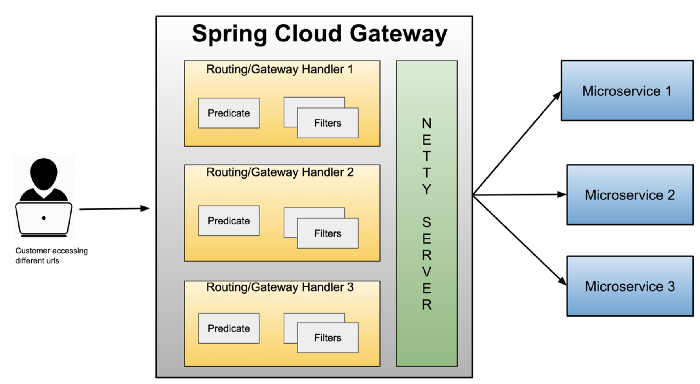
\includegraphics[width=0.8\textwidth]{Dissertation/images/api_gateway}
    \caption{Диаграмма работы API Gateway}
    \label{fig:api_gateway}
\end{figure}

Spring Cloud Circuit Breaker представляет собой библиотеку, предоставляющую абстракцию для реализации паттерна Circuit Breaker в микросервисных приложениях.
Данный паттерн используется для управления ошибками и сбоями в распределенных системах. \textit{Механизм позволяет ограничивать количество обращений к недоступным или нестабильным сервисам, перенаправляя запросы на резервные сервисы или возвращая предопределенные значения для предотвращения каскадных сбоев и минимизации времени простоя системы}.

Spring Cloud Circuit Breaker поддерживает различные реализации паттерна, включая Hystrix и Resilience4j, причем в данном проекте используется последний. Библиотека предоставляет унифицированный интерфейс для вызова удаленных сервисов через Circuit Breaker, а также обеспечивает интеграцию со Spring Cloud Discovery для автоматического обнаружения и регистрации сервисов в среде выполнения.

Eureka Service Discovery представляет собой библиотеку, реализующую механизм обнаружения и регистрации сервисов в распределенной системе. Данное решение критически важно в микросервисной архитектуре, где каждый сервис может быть развернут на различных узлах и портах, а клиентам необходима актуальная информация об адресах для доступа к сервисам.

Eureka обеспечивает возможность сервисам регистрироваться в централизованном реестре и получать информацию об адресах других сервисов.
Клиенты используют Eureka для поиска и обращения к необходимым сервисам по их логическим именам без необходимости хранения жестко закодированных адресов. Система предоставляет дополнительные функции мониторинга состояния сервисов и отслеживания изменений их конфигурации. При возникновении сбоев или перезапусках сервисов Eureka автоматически обновляет информацию в реестре, что обеспечивает устойчивость к отказам и минимизацию времени недоступности~\cite{13_davis2020}.

Разработчики могут использовать библиотеку Spring Cloud Netflix Eureka для интеграции Service Discovery в приложения на Spring.
Библиотека предоставляет декларативный подход через аннотации и конфигурационные классы для регистрации сервисов и обращения к ним через реестр Eureka.

Keycloak представляет собой комплексное решение для управления идентификацией и доступом с открытым исходным кодом.
Система предоставляет функциональность единого входа, аутентификации, авторизации, социального входа и федерации пользователей.
Keycloak поддерживает множество протоколов аутентификации, включая OAuth2, OpenID Connect, SAML и Kerberos, что обеспечивает гибкость и возможность адаптации к требованиям различных предметных областей. Административная веб-консоль Keycloak предоставляет удобный интерфейс для управления пользователями, ролями, разрешениями и клиентскими приложениями.

Apache Kafka представляет собой распределенную платформу потоковой передачи данных с открытым исходным кодом, разрабатываемую Apache Software Foundation на языках Java и Scala.
Kafka функционирует как брокер сообщений, сохраняющий данные от процессов-производителей в формате «ключ-значение».
Данные организуются в разделы в рамках различных тем~\cite{14_niya2019}. Внутри каждого раздела сообщения строго упорядочены по смещениям, определяющим позицию сообщения, и индексируются с сохранением временных меток.
Процессы-потребители осуществляют чтение сообщений из разделов.
Для потоковой обработки Kafka предоставляет Streams API, позволяющий разрабатывать Java-приложения для обработки потоков данных.

Схема работы представлена на рисунке~\ref{fig:kafka_architecture}.
\begin{figure}[htbp]
    \centering
    % Placeholder для диаграммы архитектуры Apache Kafka
    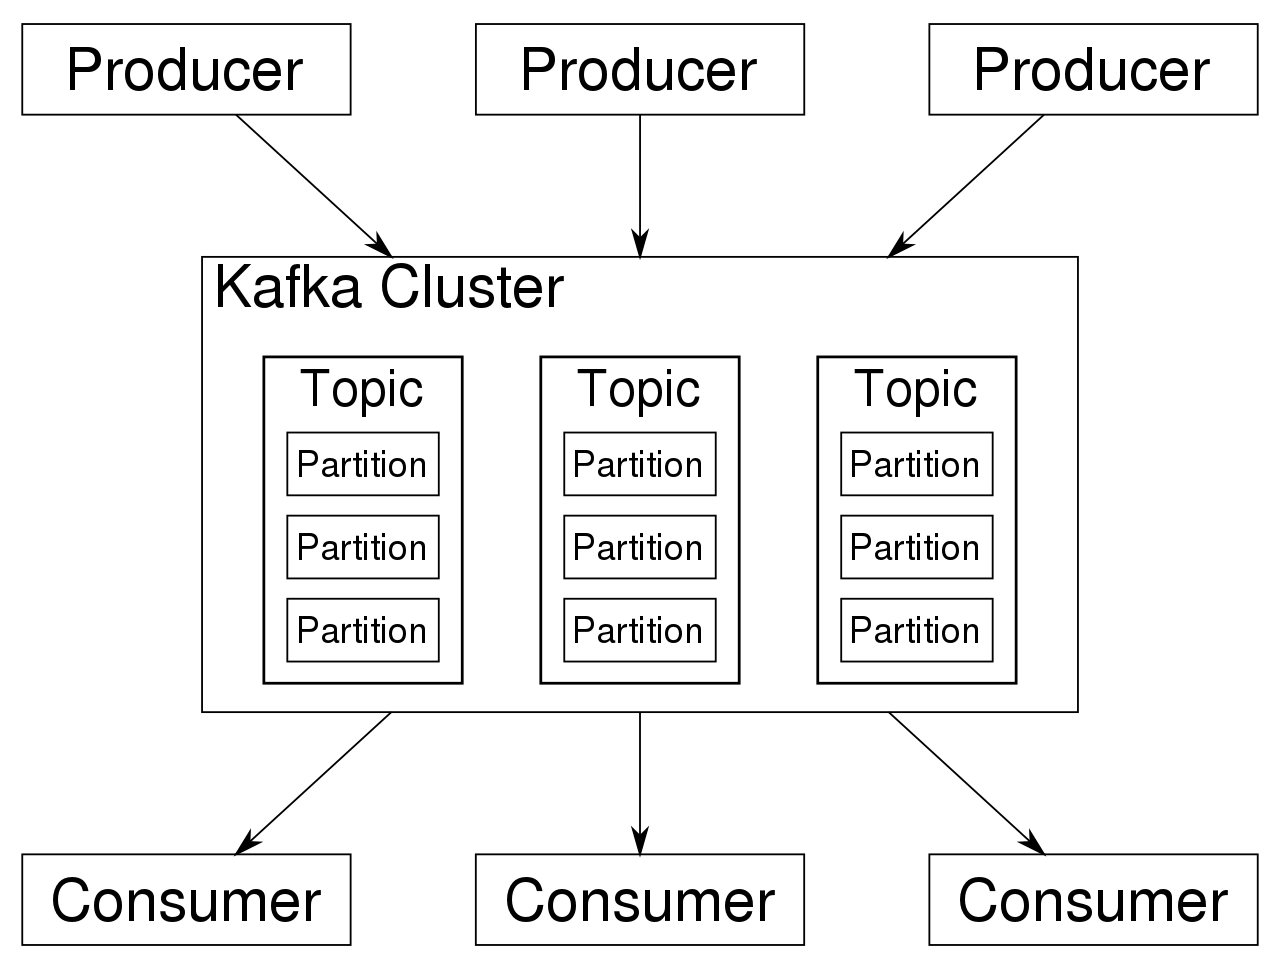
\includegraphics[width=0.7\textwidth]{Dissertation/images/kafka_scheme}
    \caption{Архитектура Apache Kafka}
    \label{fig:kafka_architecture}
\end{figure}

\subsection{Проектирование структуры приложения}

После определения современного технологического стека необходимо спроектировать архитектуру продукта для формирования стратегии развития и устранения потенциальных противоречий на этапе проектирования.

В основу архитектурного решения положен подход микросервисной архитектуры, который в сравнении со стандартным монолитным RESTful API обладает рядом существенных преимуществ.
Гибкость микросервисной архитектуры проявляется в возможности независимого добавления, удаления или модификации отдельных сервисов без влияния на функционирование остальной системы. \textit{Данная характеристика критически важна для проекта, предполагающего распределенную разработку несколькими группами из различных географических локаций, обеспечивая эффективное делегирование обязанностей}.

Масштабируемость реализуется через возможность независимого масштабирования каждого микросервиса, что позволяет оперативно реагировать на изменение нагрузки. Учитывая неравномерное использование различных сервисов в разные временные периоды, данный подход обеспечивает оптимальное использование вычислительных ресурсов~\cite{15_dragoni2017}.

Удобство командной разработки обеспечивается возможностью независимой разработки, тестирования и развертывания каждого микросервиса. Принимая во внимание планируемую интеграцию со сторонними сервисами для расширения технологической среды исторических исследований, данное преимущество приобретает особую актуальность.

Высокая доступность достигается через размещение микросервисов в специализированных кластерах с поддержкой репликации и оркестрации. Механизмы автоматического восстановления отдельных сервисов в случае их отказа обеспечивают устойчивость системы к сбоям~\cite{16_schermann2016}.

На основании проведенного анализа была разработана архитектурная схема проекта, отражающая основные компоненты и их взаимосвязи, она представлена на рисунке~\ref{fig:microservices_schema}.

\begin{figure}[htbp]
    \centering
    % Placeholder для схемы микросервисной архитектуры проекта
    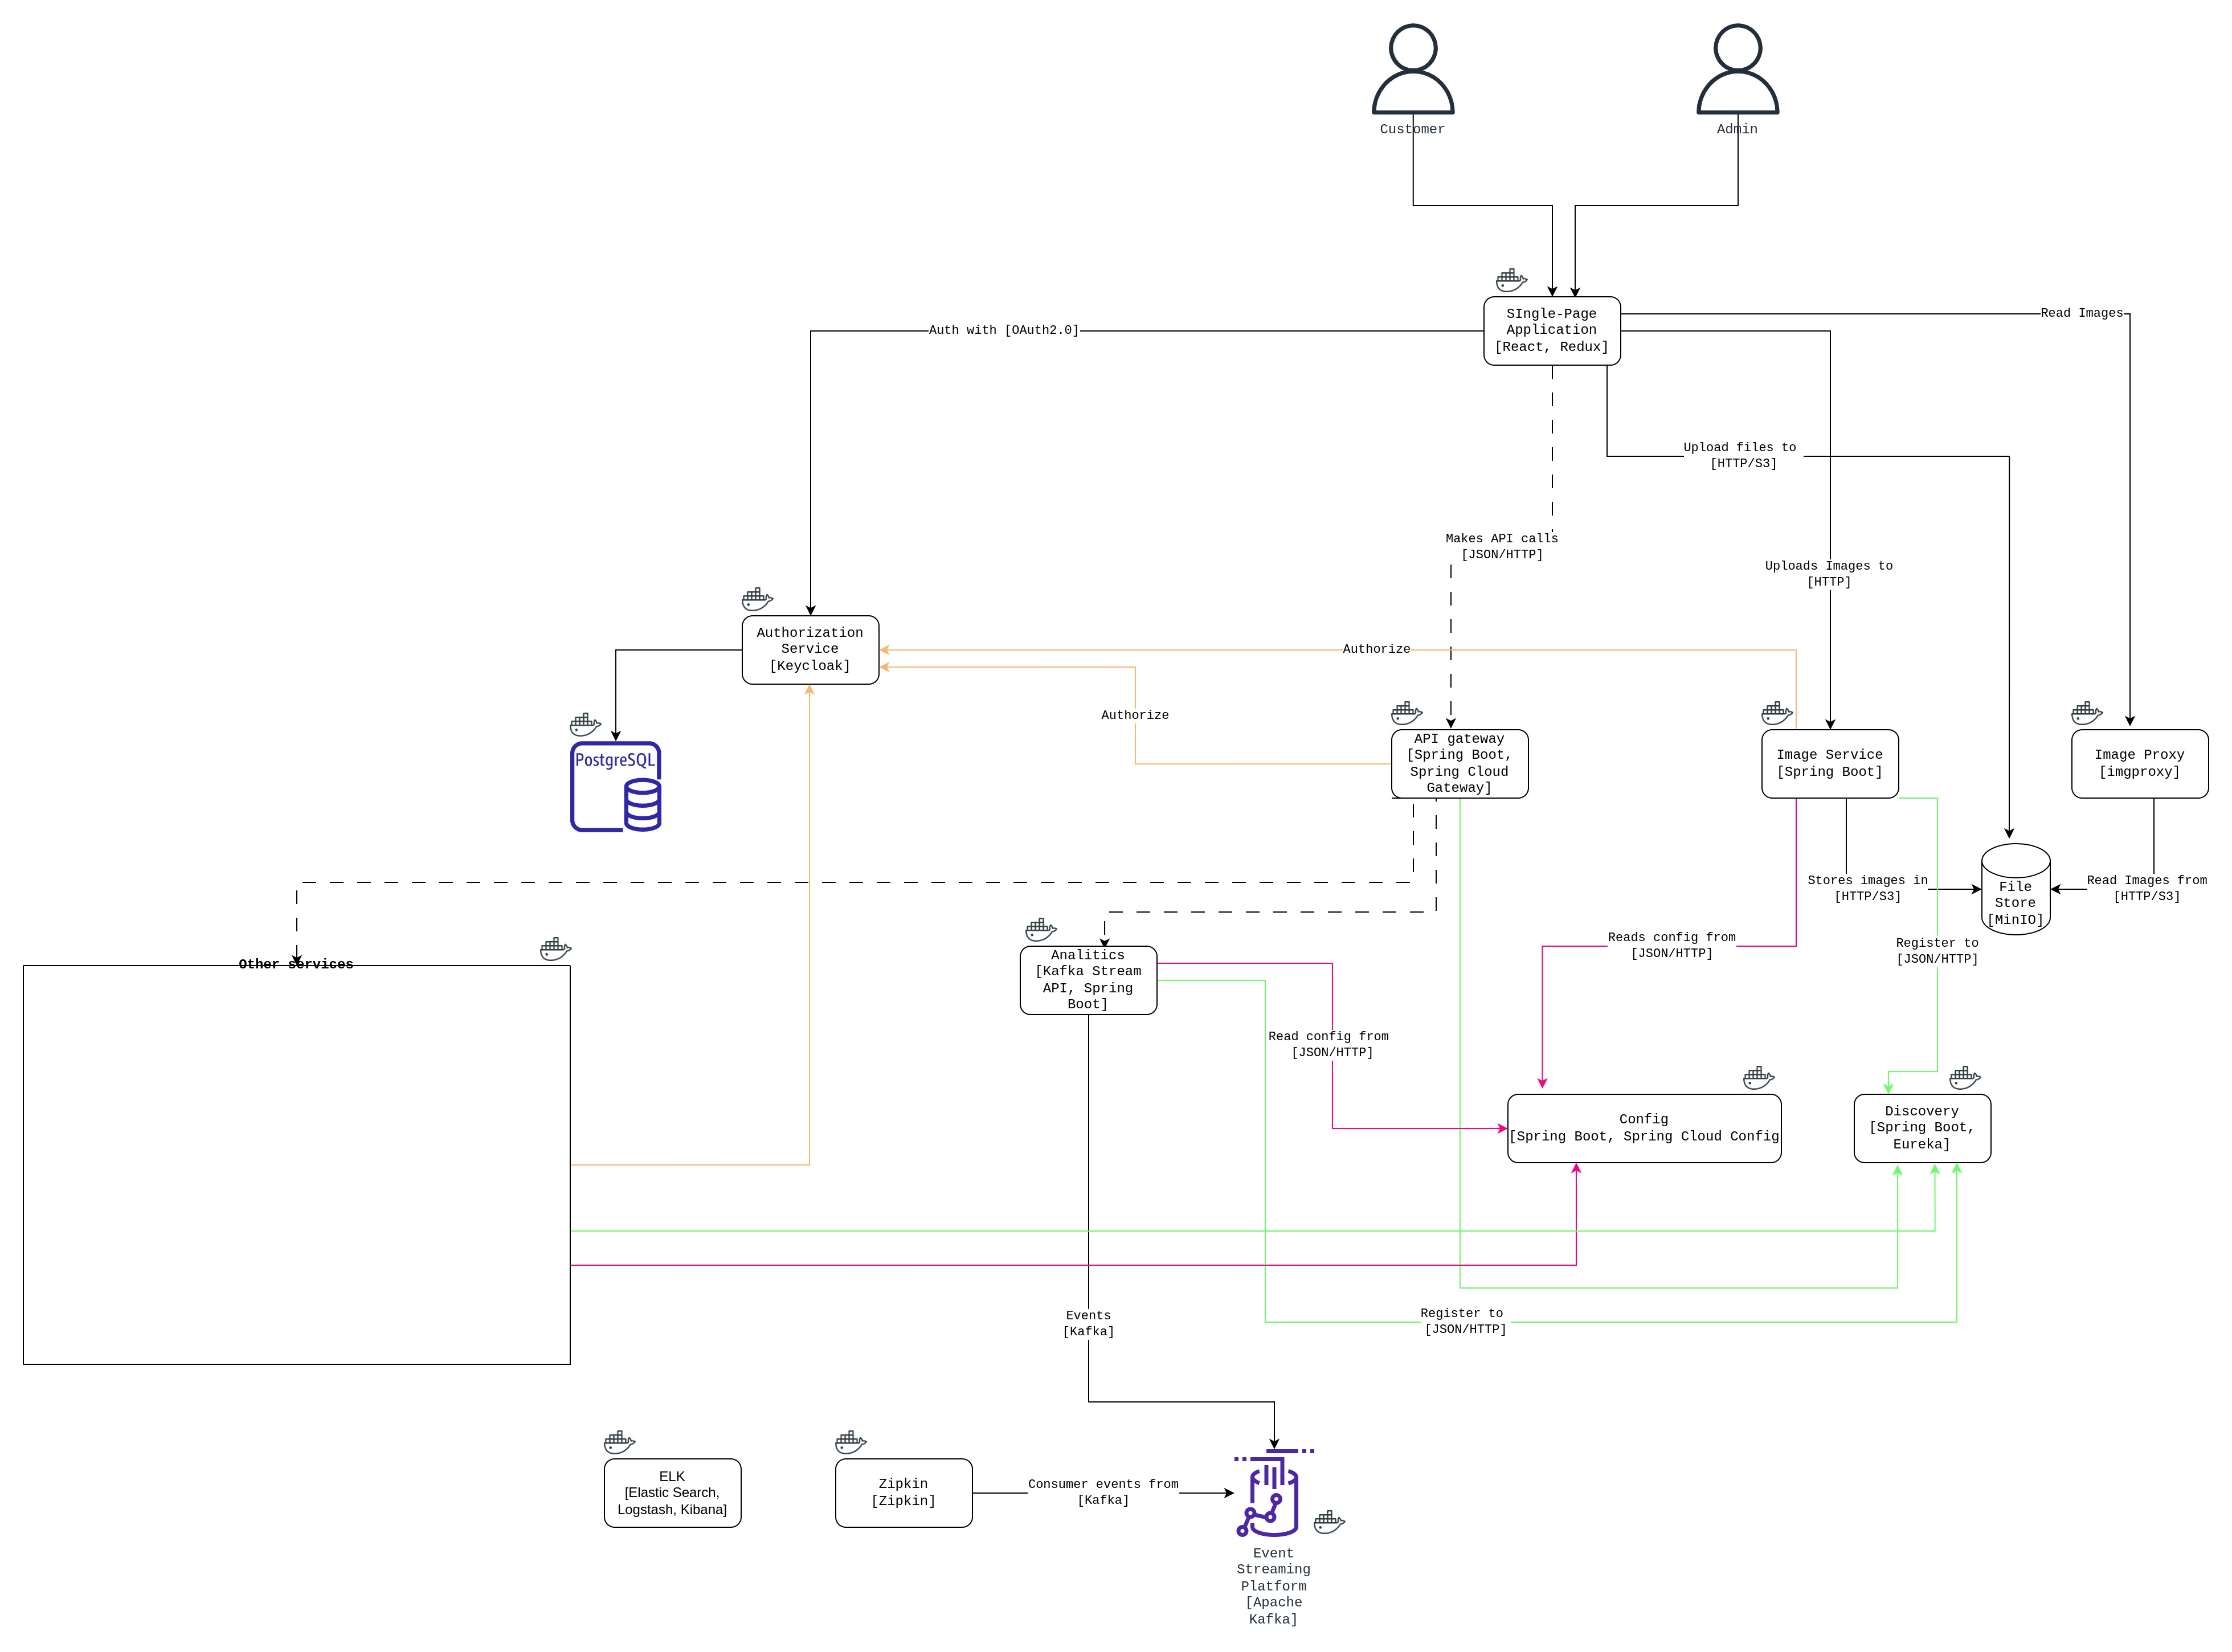
\includegraphics[width=0.7\textwidth]{Dissertation/images/project_scheme}
    \caption{Схема микросервисной архитектуры проекта}
    \label{fig:microservices_schema}
\end{figure}

\subsubsection{Служба конфигурации: архитектурные принципы и реализация}

Внедрение сервера конфигурации в инфраструктуру микросервисов обладает критической важностью для обеспечения стабильности, управляемости и масштабируемости распределенных систем. Данный компонент представляет собой централизованное решение для управления конфигурационными параметрами, обеспечивающее консистентность и согласованность между различными компонентами системы.

Централизованное управление настройками множества микросервисов решает проблему консистентности конфигураций в условиях, когда каждый микросервис обладает уникальными параметрами. \textit{Это особенно критично в распределенных системах, где конфигурационные изменения должны оперативно и синхронно применяться ко всем компонентам инфраструктуры}.

Централизованное хранение конфигураций существенно упрощает процессы обновления и развертывания микросервисов.
Возможность динамического изменения параметров конфигурации без перезапуска микросервисов сокращает время простоя системы. Данная характеристика является критически важной для бизнес-критичных приложений, требующих высокой доступности.

Сервер конфигурации существенно улучшает безопасность системы через централизованное управление конфиденциальными данными.
Ключи API и пароли хранятся в зашифрованном виде и предоставляются исключительно авторизованным микросервисам. \textit{Данный подход минимизирует риски утечек данных и упрощает управление доступом к чувствительной информации}.

Улучшение масштабируемости достигается через эффективное управление конфигурациями при росте количества микросервисов. Сервер конфигурации обеспечивает быстрый и гибкий доступ к необходимым параметрам независимо от масштаба системы.

\paragraph{Критерии выбора сервера конфигурации}

При выборе сервера конфигурации для платформы анализа исторических данных необходимо учитывать комплекс критериев, обеспечивающих надежную и эффективную работу инфраструктуры.
Первостепенным требованием является обеспечение высокой доступности через механизмы автоматического восстановления и горизонтального масштабирования. Критически важными факторами являются минимизация задержек при доступе к конфигурационным файлам и поддержка различных форматов данных, включая JSON и YAML.

Лицензионные условия использования требуют тщательного анализа. \textit{Необходимо детальное изучение условий лицензирования и возможностей использования в коммерческих и некоммерческих проектах}.
Обязательным требованием является поддержка шифрования конфигураций как в состоянии покоя, так и при передаче данных. Наличие активного сообщества разработчиков, хотя и является опциональным требованием, существенно влияет на долгосрочную поддержку и развитие продукта.

\paragraph{Сравнительный анализ решений для управления конфигурациями}

Для обоснованного выбора решения проведен сравнительный анализ трех наиболее распространенных инструментов управления конфигурациями в распределенных системах: Consul, etcd и Spring Cloud Config. Каждое из данных решений обладает уникальными характеристиками, определяющими область их оптимального применения.

Consul, разработанный компанией HashiCorp, представляет собой комплексную распределенную систему, объединяющую функции управления конфигурациями, обнаружения сервисов и организации сервисной сети. Consul предоставляет интегрированную функциональность для регистрации сервисов, мониторинга их состояния, распределенного хранения конфигураций и автоматизации сетевого взаимодействия.

Преимущества Consul включают автоматическое обнаружение и регистрацию сервисов, встроенные механизмы проверки состояния, использование распределенного KV-хранилища и поддержку функций сервисной сети с управлением сетевыми политиками. \textit{Однако сложность настройки и интеграции, особенно в крупных кластерах, а также высокие требования к ресурсам могут ограничивать применение в небольших проектах}.

etcd, разработанный CoreOS, представляет собой распределенное хранилище конфигураций, основанное на алгоритме консенсуса Raft. \textit{Данное решение широко используется в экосистеме Kubernetes для хранения конфигурационных данных и метаданных}.
etcd обеспечивает строгое согласование данных, высокую производительность, низкую задержку доступа и простое API. Глубокая интеграция с Kubernetes делает его естественным выбором для контейнеризованных приложений. \textit{Ограничения включают отсутствие встроенных механизмов обнаружения сервисов и сложность управления кластером в больших масштабах}.

Spring Cloud Config представляет собой специализированный инструмент для управления конфигурациями в облачных приложениях экосистемы Spring. \textit{Решение обеспечивает централизованное управление конфигурационными файлами с поддержкой динамических изменений}.
Глубокая интеграция с экосистемой Spring, централизованное управление и поддержка версионирования через системы контроля версий являются ключевыми преимуществами. \textit{Ограничения включают узкую специализацию на управлении конфигурациями и оптимизацию исключительно для Spring-приложений}.

\paragraph{Реализация Configuration Service}

Configuration Service обеспечивает поддержку управления внешними конфигурациями в распределенной системе. Хранилище конфигураций версионируется под контролем Git и поддерживает изменения во время выполнения.
Сервер предоставляет REST API для получения конфигураций микросервисами.

Конфигурационные файлы в текущей реализации размещаются в classpath.
Сервер поддерживает шифрование и расшифровку значений свойств. По умолчанию используется симметричная криптография, а при запуске с профилем <<docker>> применяется асимметричная криптография.

Поддержка шифрования позволяет использовать публичные репозитории для хранения конфиденциальных данных.
Зашифрованные значения маркируются префиксом \texttt{\{cipher\}}. \textit{Для симметричной криптографии необходима установка свойства} \texttt{encrypt.key}.
Асимметричная криптография требует настройки хранилища ключей через утилиту Java keytool:

\begin{lstlisting}
keytool -genkeypair -alias configkey -keyalg RSA
-dname "CN=Web Server,C=RU,S=OH" -keypass cfg-password
-keystore keystore.jks -storepass secure-keystore-password
\end{lstlisting}

\paragraph{Заключение по выбору сервера конфигурации}

Выбор инструмента для управления конфигурациями определяется спецификой проекта и архитектурными требованиями. Consul оптимален для комплексных систем с требованиями управления сетевой политикой. etcd представляет лучший выбор для высокопроизводительного хранения данных в Kubernetes-окружении. Spring Cloud Config является идеальным решением для централизованного управления конфигурациями в Spring-приложениях, что обосновывает его выбор для данного проекта.

\subsubsection{Служба обнаружения}

В качестве реестра сервисов используется Netflix Eureka, предоставляющая REST API для регистрации и обнаружения сервисов.
Реестр служб обеспечивает балансировку нагрузки на стороне клиента и отделяет поставщиков услуг от потребителей без использования DNS.

Каждая служба регистрируется в реестре и периодически отправляет сигналы жизнедеятельности для подтверждения доступности. \textit{Механизм heartbeat обеспечивает актуальность информации о состоянии сервисов в реестре}.
Клиенты запрашивают реестр для получения списка доступных экземпляров службы.

После получения списка доступных экземпляров клиент применяет алгоритм балансировки нагрузки для выбора целевого экземпляра. Локальное кеширование регистраций Eureka на стороне клиента минимизирует количество обращений к реестру и повышает производительность системы.

\subsubsection{API Gateway: маршрутизация и фильтрация}

В контексте современных цифровых экосистем API Gateway представляет собой критически важное архитектурное решение, обеспечивающее рационализацию и организацию потока данных между клиентами и целевыми микросервисами.
Данный компонент предоставляет комплексную функциональность маршрутизации, фильтрации и авторизации трафика. API Gateway является одним из ключевых элементов микросервисной архитектуры, обеспечивающим организацию как внутренних, так и внешних взаимодействий между компонентами системы.

\paragraph{Прямое взаимодействие клиента и сервиса}

В определенных архитектурных сценариях рассматривается возможность прямого взаимодействия клиента с микросервисами.
Данный подход предполагает непосредственную отправку запросов клиентским приложением к отдельным микросервисам без промежуточных компонентов.
Каждый микросервис предоставляет общедоступный эндпоинт с индивидуальным TCP-портом для обеспечения прямого доступа.

Такой подход отражен на рисунке~\ref{fig:direct_client_service}.
\begin{figure}[htbp]
    \centering
    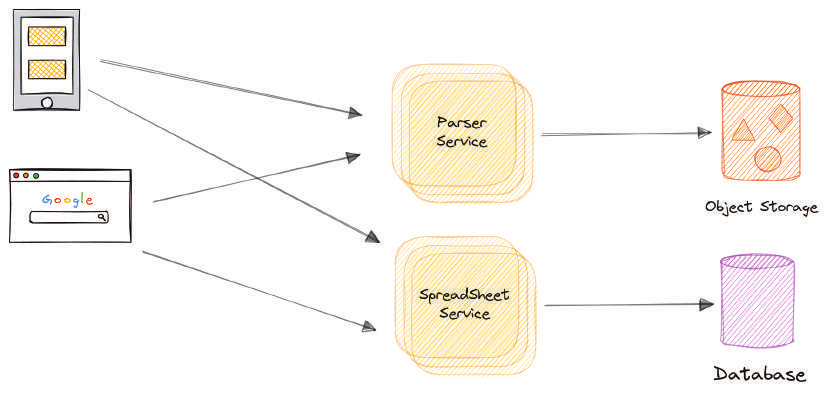
\includegraphics[width=0.7\textwidth]{Dissertation/images/wo_gateway}
    \caption{Схема прямого взаимодействия клиента и микросервиса}
    \label{fig:direct_client_service}
\end{figure}

При прямом взаимодействии возникает необходимость в механизмах управления трафиком и обеспечения безопасности~\cite{trebichavsky2021}. \textit{В данном контексте могут применяться балансировщики нагрузки или контроллеры доставки приложений, обеспечивающие равномерное распределение запросов и базовый уровень защиты через SSL-шифрование}.

Однако при создании масштабных микросервисных приложений, особенно при взаимодействии с мобильными приложениями или одностраничными веб-приложениями, возникает комплекс критических проблем~\cite{microsoft_api_gateway}. Масштабирование системы требует минимизации обращений к серверной части, управления сквозными задачами авторизации и безопасности, создания специализированных фасадов для различных типов клиентов~\cite{newman2015building}.

Прямое соединение клиента с сервисами приводит к нелинейному увеличению сложности взаимодействия. \textit{Необходимость поддержания соединения на протяжении всего запроса существенно увеличивает нагрузку на сетевые ресурсы}.
Отсутствие централизованного механизма контроля аутентификации создает серьезные проблемы безопасности. \textit{Поддержание единой политики безопасности становится практически невозможным из-за необходимости реализации собственной системы безопасности в каждом сервисе}.

Прямое взаимодействие существенно усложняет процессы обновления и масштабирования.
Внесение изменений в микросервисы требует обновления всех клиентских приложений, что представляет собой трудоемкий и времязатратный процесс.

\paragraph{Паттерн API Gateway}

Шаблон API Gateway представляет собой архитектурную концепцию для масштабных микросервисных приложений с множественными клиентскими интерфейсами.
API Gateway функционирует как централизованная точка входа для определенных кластеров микросервисов. Данный паттерн, аналогичный концепции фасада в объектно-ориентированном проектировании, является фундаментальным элементом децентрализованных систем.

API Gateway, размещенный между клиентскими приложениями и микросервисами, функционирует как обратный прокси-сервер, маршрутизирующий запросы к соответствующим сервисам~\cite{zhao2018management}. Помимо маршрутизации, API Gateway обеспечивает комплексную функциональность, включающую аутентификацию, SSL-терминацию и кэширование.

Примерная схема изображена на рисунке~\ref{fig:api_gateway_interaction}
\begin{figure}[htbp]
    \centering
    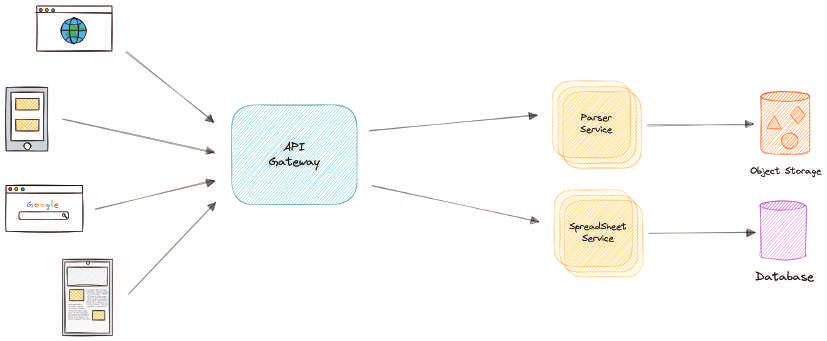
\includegraphics[width=0.7\textwidth]{Dissertation/images/gateway_project_scheme}
    \caption{Схема взаимодействия клиентов с микросервисами через API Gateway}
    \label{fig:api_gateway_interaction}
\end{figure}

Использование единого API Gateway для обслуживания различных клиентских приложений может создавать риски в плане масштабирования и поддержки. Разнообразие требований клиентских приложений может привести к превращению API Gateway в монолитный сервис.
Рекомендуется разделение API Gateway на несколько служб в соответствии с бизнес-границами и потребностями клиентов.

\paragraph{Backend for Frontend (BFF)}

Разделение уровня API Gateway на несколько компонентов основывается на создании специализированных эндпоинтов для различных типов клиентов(рис~\ref{fig:bff_pattern}). Паттерн Backend for Frontend предполагает предоставление API Gateway специализированного интерфейса для конкретного типа клиентского приложения~\cite{alkhodary2023evaluation}.

\begin{figure}[htbp]
    \centering
    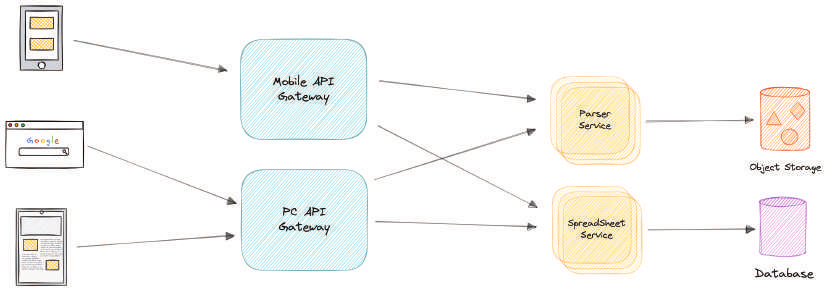
\includegraphics[width=0.7\textwidth]{Dissertation/images/bff}
    \caption{Архитектурный паттерн Backend for Frontend (BFF)}
    \label{fig:bff_pattern}
\end{figure}

Для платформ с множеством сервисов применение агрегации становится критически важным для объединения низкоуровневых вызовов~\cite{newman2015building}.
Один вызов к BFF-шлюзу порождает серию низкоуровневых обращений к различным микросервисам. В контексте платформы аналитики исторических данных это может включать получение координат церквей из определенного уезда для визуализации перемещения рукописей.

Оптимизация ресурсов достигается через максимальную параллелизацию вызовов. После завершения начального вызова к сервису поиска координат последующие обращения к другим сервисам выполняются параллельно для минимизации общего времени обработки(рис.~\ref{fig:bff_parallel_processing}).

\begin{figure}[htbp]
    \centering
    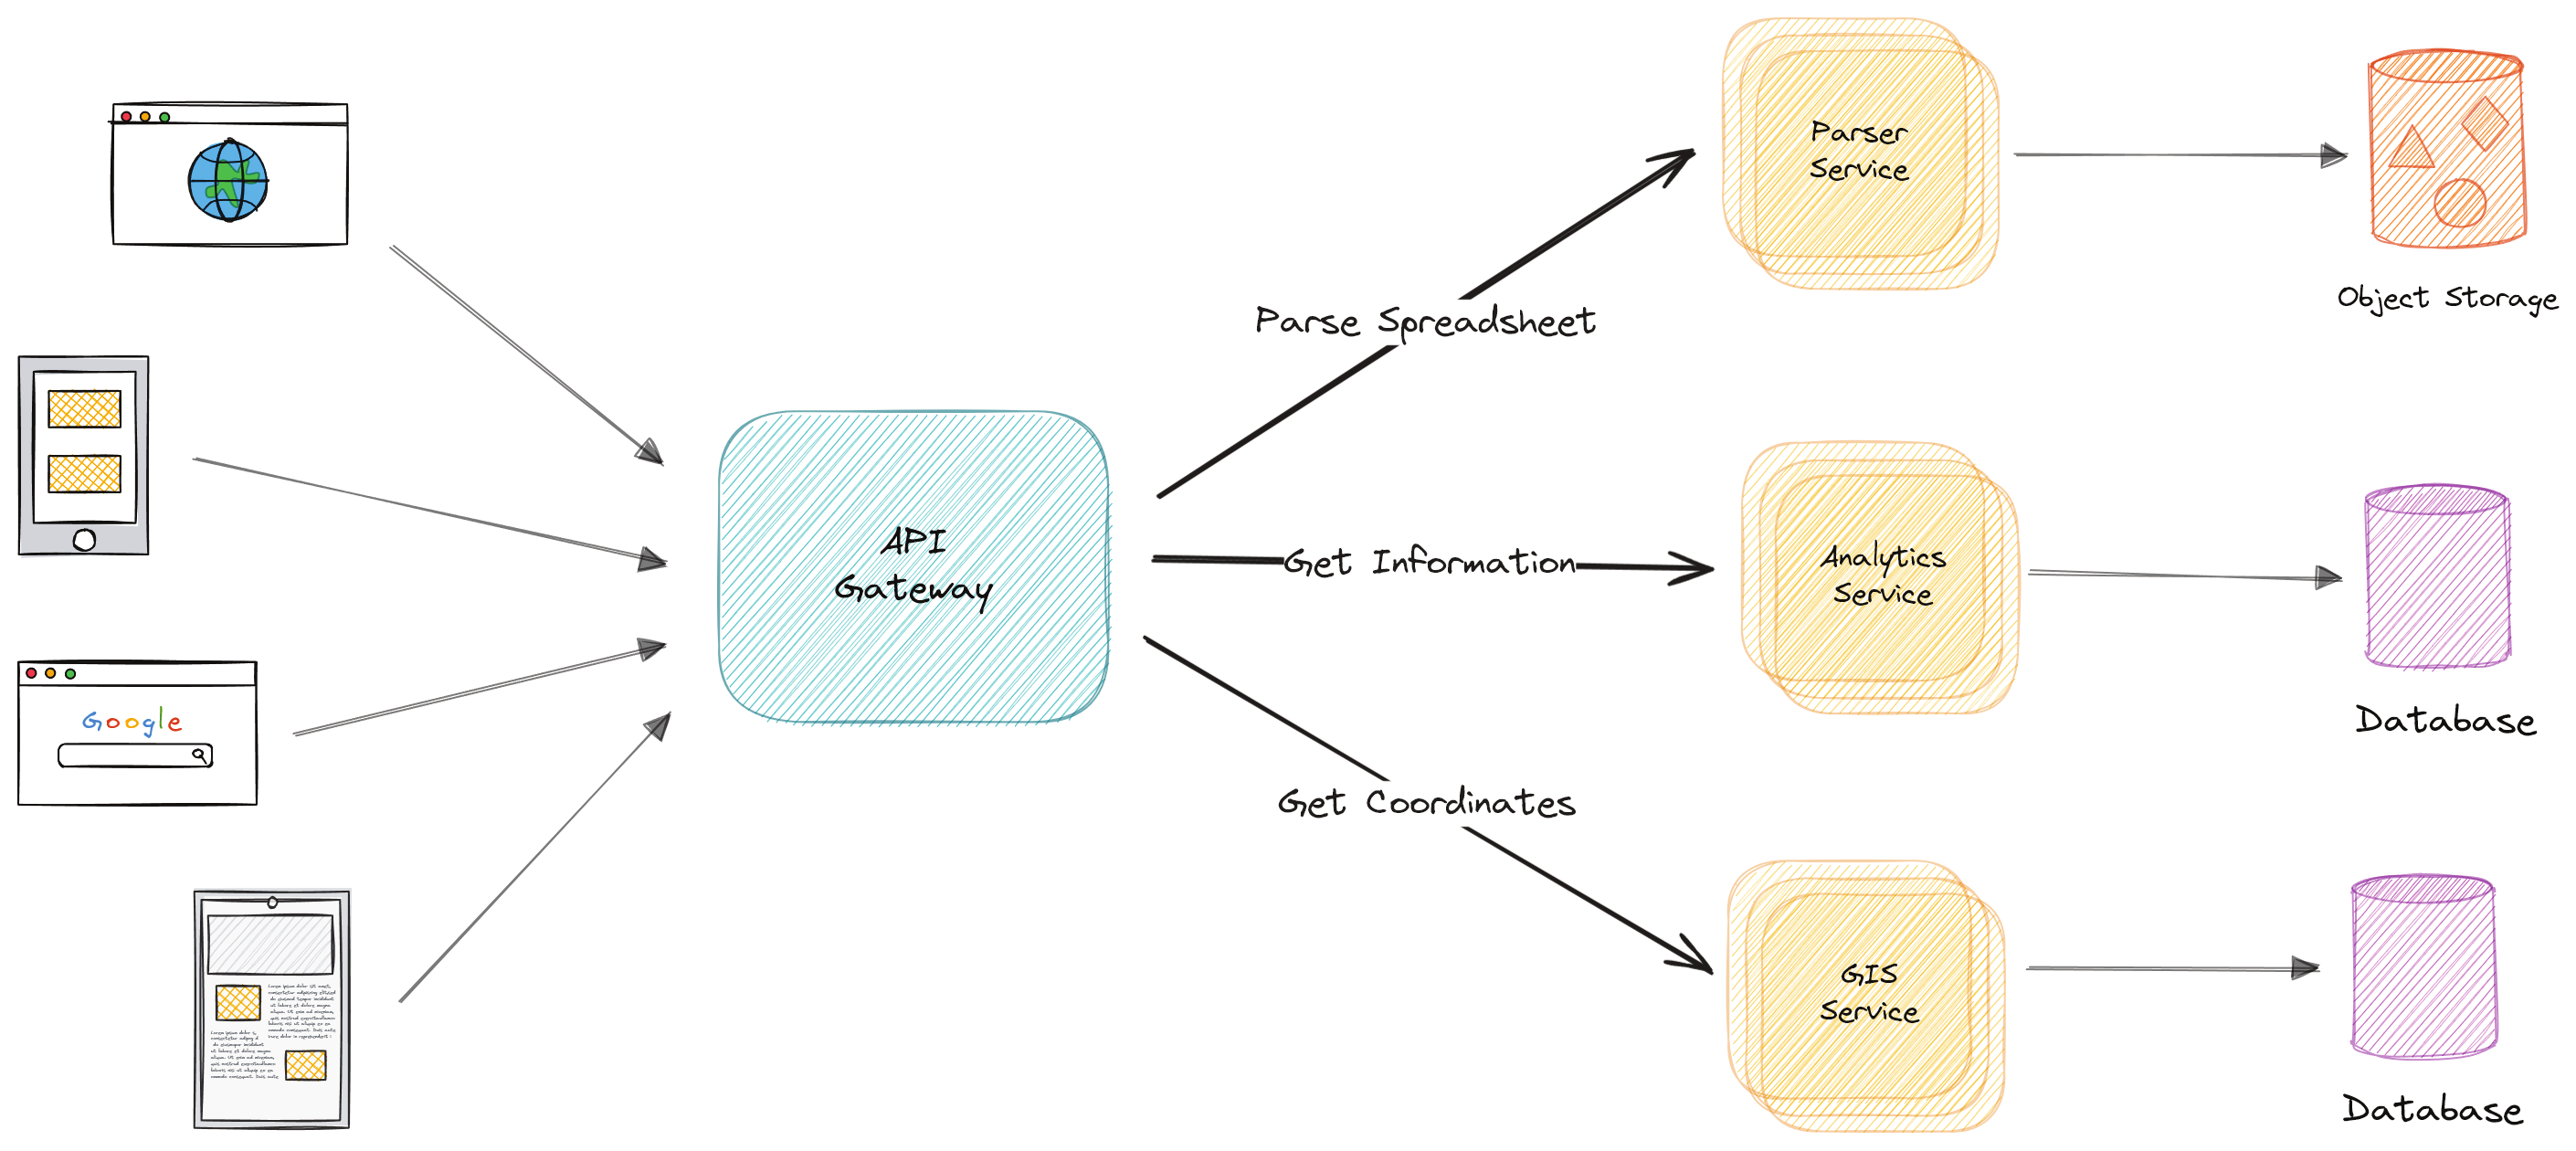
\includegraphics[width=0.7\textwidth]{Dissertation/images/bff_par}
    \caption{Схема параллельной обработки запросов в BFF}
    \label{fig:bff_parallel_processing}
\end{figure}

\paragraph{Сравнительный анализ решений API Gateway}

Сравнительный анализ решений API Gateway основывается на критериях производительности, масштабируемости, безопасности, интеграции, удобства использования и поддержки сообщества. Анализ включает Spring Cloud Gateway, Kong, Amazon API Gateway, Apigee и NGINX.

Spring Cloud Gateway демонстрирует высокую производительность благодаря реактивной архитектуре на основе Spring WebFlux, обеспечивающей асинхронную обработку и высокую пропускную способность.
Kong характеризуется аналогичной производительностью благодаря использованию NGINX и LuaJIT. Spring Cloud Gateway легко масштабируется в экосистеме Spring Cloud с поддержкой кластеризации и интеграции с системами оркестрации~\cite{carnell2021spring}. \textit{Kong поддерживает горизонтальное масштабирование и интеграцию с контейнерными оркестраторами}.

Spring Cloud Gateway поддерживает интеграцию с решениями аутентификации и авторизации, включая OAuth2 и JWT. \textit{Kong обладает комплексными функциями безопасности, включающими SSL/TLS шифрование и контроль доступа на уровне API}.

Spring Cloud Gateway, благодаря высокой производительности, простоте интеграции с экосистемой Spring и обширному сообществу, является оптимальным выбором для проектов на базе Spring. \textit{Решение обеспечивает необходимую гибкость, масштабируемость и безопасность для современных микросервисных архитектур}.

\paragraph{Spring Cloud Gateway: архитектурные особенности}

Для платформы аналитики исторических данных API Gateway должен обеспечивать маршрутизацию запросов в различные версии сервисов, поддержку OAuth 2.0 для передачи информации о пользователе, сбор метрик и логирование.
Spring Cloud Gateway полностью соответствует данным требованиям~\cite{spring_cloud_gateway}. \textit{Ключевым преимуществом является работа в неблокирующем режиме}.

Неблокирующая архитектура, реализованная на основе Netty и проекта Reactor, представляет собой асинхронный фреймворк с циклами событий. Архитектура может использовать минимальное количество потоков, где каждый процессорный поток управляет циклом событий с каналами для обработки входящих соединений.

Запрос поступает через HTTP в канал, обрабатывается циклом событий и передается в приложение WebFlux как объект ServerHttpRequest. Обработка происходит в неблокирующем режиме: цикл событий создает флаг ожидания ответа и готов принимать новые запросы.
WebFlux оборачивает запрос в ServerWebExchange и передает его через цепочку обработчиков до WebClient.

В процессе взаимодействия микросервисов при синхронных вызовах существует вероятность недоступности или высокой задержки~\cite{richardson_circuit_breaker}. Это может привести к блокировке ресурсов вызывающей стороны и неспособности обработки других запросов.

Для обеспечения надежного взаимодействия используется прокси-сервер, функционирующий по принципу электрического выключателя~\cite{richardson2018microservices}. При достижении порога последовательных сбоев происходит автоматическое срабатывание, и в течение периода ожидания все попытки обращения завершаются неудачей.
После истечения времени ожидания пропускается ограниченное количество тестовых запросов.

API-шлюз использует паттерн Circuit Breaker, реализованный через Spring Cloud Circuit Breaker и Resilience4j.

\subsection{Проектирование безопасности}

Обеспечение максимальной безопасности и конфиденциальности данных пользователей является приоритетной задачей проекта.
Реализован отдельный авторизационный сервис, функционирующий по протоколам OAuth2.0 и OpenID~\cite{18_hardt2012,openid_foundation2014}.

OAuth2 представляет собой протокол авторизации для безопасной передачи данных между сторонними сервисами~\cite{richer2017}.
Протокол позволяет пользователям предоставлять доступ к данным без передачи паролей. Приложение получает токен доступа от сервера авторизации для последующего доступа к ресурсам пользователя~\cite{18_hardt2012}.
Важные аспекты безопасности OAuth2.0 детально рассмотрены в специальной спецификации угроз и мер безопасности~\cite{lodderstedt2013}, а формальный анализ безопасности протокола представлен в работе~\cite{fett2016}.

OpenID представляет открытый стандарт децентрализованной системы аутентификации, позволяющий создать единую учетную запись для множества интернет-ресурсов через услуги третьих лиц~\cite{19_weingartner2017,sakimura2015}.
OpenID Connect функционирует как идентификационный слой поверх OAuth 2.0, обеспечивая надежную аутентификацию пользователей~\cite{openid_foundation2014}.

На рисунке~\ref{fig:openid_diagram} можно увидеть диаграмму деятельности OpenID.
\begin{figure}[htbp]
    \centering
    % Placeholder для диаграммы деятельности OpenID
    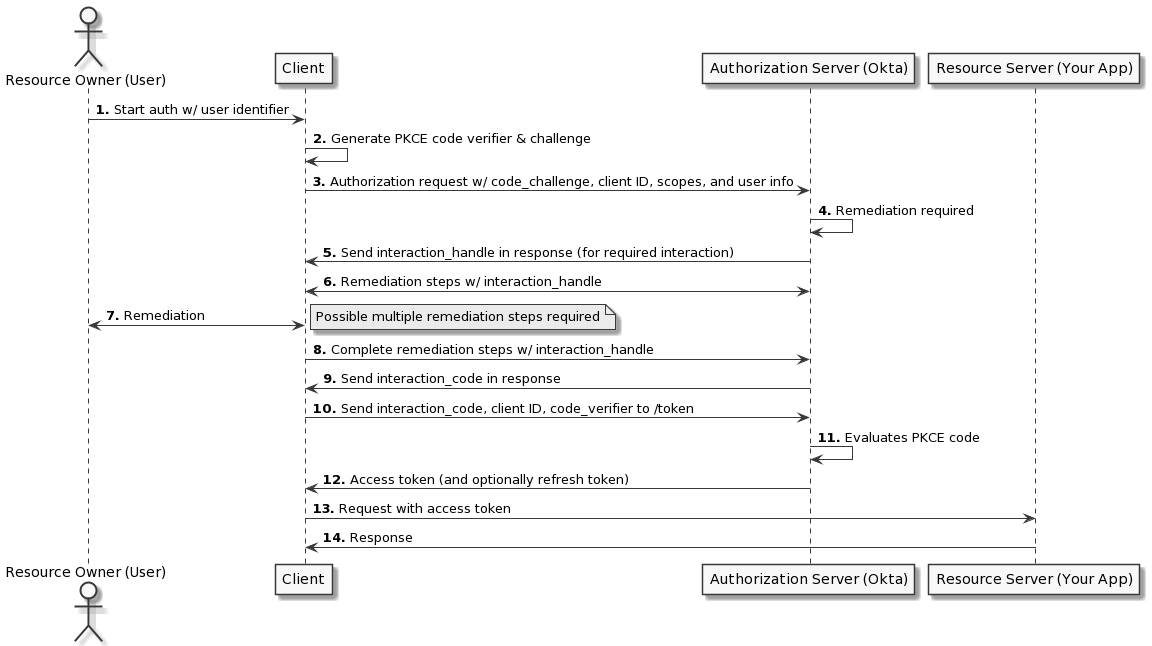
\includegraphics[width=0.7\textwidth]{Dissertation/images/openId_scheme}
    \caption{Диаграмма деятельности OpenID}
    \label{fig:openid_diagram}
\end{figure}

Реализация системы безопасности на основе OpenID и OAuth2 обеспечивает современный уровень защиты данных и соответствует международным стандартам информационной безопасности~\cite{fett2016,19_weingartner2017}.
           % Глава 1
    \chapter{Практическая часть}


\section{Внедрение API Gateway в архитектуру информационно-аналитической системы}

\subsection{Анализ требований и постановка исследовательских задач}

Разработка архитектурного решения для информационно-аналитического ресурса «Православный ландшафт таежной Сибири» инициируется комплексным анализом функциональных и нефункциональных требований к распределенной системе обработки исторических данных. Фундаментальным требованием выступает обеспечение высокодоступного и отказоустойчивого доступа к гетерогенным массивам исторической информации, что обусловливает необходимость применения современных архитектурных паттернов и технологических решений.

Требование масштабируемости определяется экспоненциальным ростом объемов обрабатываемых данных и интенсивности пользовательских запросов, что предполагает реализацию механизмов горизонтального масштабирования и динамического распределения вычислительной нагрузки. Особую значимость приобретает обеспечение информационной безопасности и защиты персональных данных в контексте обработки исторических документов, содержащих конфиденциальную информацию о религиозных объектах и персоналиях. Гибкость маршрутизации и обработки разнородных запросов представляет собой критически важное требование, обусловленное полиморфной природой аналитических задач и множественностью клиентских интерфейсов.

\subsection{Компонентная декомпозиция архитектурного решения}

Архитектурная организация системы базируется на принципах микросервисной декомпозиции с выделением следующих фундаментальных компонентов. Spring Cloud Gateway выступает в качестве центрального координирующего элемента, реализующего функции интеллектуальной маршрутизации запросов и применения комплексных политик безопасности. Данный компонент обеспечивает абстрагирование внутренней топологии микросервисной экосистемы от внешних потребителей, реализуя принцип инкапсуляции на архитектурном уровне.

Микросервисная инфраструктура представлена специализированными вычислительными модулями, каждый из которых инкапсулирует определенную область предметной логики. Сервисы обработки исторических данных реализуют алгоритмы семантического анализа и контекстуальной интерпретации архивных документов. Подсистема управления пользовательскими контекстами обеспечивает персонализацию аналитических процессов и поддержку многопользовательских сценариев работы. Модули генерации отчетов применяют методы визуальной аналитики для представления результатов исследований в различных форматах.

Персистентный уровень архитектуры реализован через гибридную модель хранения, сочетающую реляционные системы управления базами данных для структурированной информации о православных объектах культурного наследия и документо-ориентированные хранилища для неструктурированных исторических материалов. Применение полиглотной персистентности позволяет оптимизировать характеристики производительности для различных типов аналитических запросов. Интерфейсный уровень представлен совокупностью веб-приложений, обеспечивающих многоканальный доступ к функциональности системы с учетом специфики различных категорий пользователей.


\section{Архитектурная организация микросервисной системы аналитики исторических данных}

\subsection{Компонентная структура информационно-аналитического ресурса}

Архитектура современных информационно-аналитических систем требует комплексного подхода к организации вычислительных ресурсов и обработке данных. В рамках разработки онлайн-ресурса «Православный ландшафт таежной Сибири» была спроектирована микросервисная архитектура, обеспечивающая модульность, масштабируемость и отказоустойчивость системы. Каждый микросервис в данной архитектуре представляет собой автономную функциональную единицу, ответственную за конкретную область предметной логики: обработку исторических данных, управление пользовательскими сессиями, генерацию аналитических отчетов и визуализацию геопространственной информации.

Персистентный слой системы реализован посредством гибридного подхода к хранению данных, сочетающего реляционные и документо-ориентированные базы данных для оптимального представления структурированной информации о православных объектах культурного наследия и неструктурированных исторических документов. Интерфейсный уровень представлен веб-приложениями, обеспечивающими многоканальный доступ к функциональности системы.

\subsection{Проблематика архитектуры прямого обращения к микросервисам}

До внедрения централизованного API-шлюза архитектура системы базировалась на принципе прямой маршрутизации запросов к отдельным микросервисам. Данный подход демонстрировал ряд существенных ограничений, препятствующих эффективному функционированию распределенной системы.

Первичной проблемой являлось обеспечение информационной безопасности. Прямой доступ к микросервисам экспоненциально увеличивал поверхность атаки системы, создавая множественные векторы потенциальных угроз. Отсутствие единой точки контроля делало практически невозможным применение консистентных политик безопасности и мониторинга аномальной активности в режиме реального времени. Каждый микросервис требовал индивидуальной реализации механизмов аутентификации и авторизации, что приводило к дублированию кода и повышало вероятность возникновения уязвимостей.

Версионирование API представляло собой отдельную категорию сложностей. Наличие множественных эндпоинтов у каждого микросервиса, включая различные версии интерфейсов в рамках одного сервиса, создавало проблему управления жизненным циклом API. Клиентские приложения вынуждены были поддерживать сложную логику маршрутизации и обработки различных версий интерфейсов, что существенно усложняло процесс разработки и поддержки.

Дополнительно следует отметить проблему кросс-функциональных требований (cross-cutting concerns), таких как логирование, мониторинг производительности и обработка ошибок, которые требовали реализации в каждом микросервисе отдельно. Это приводило к нарушению принципа DRY (Don't Repeat Yourself) и усложняло поддержку единообразия системы.
Архитектурная схема работы проекта до внедрения выглядела сле-
дующим образом~\ref{fig:wo-gateway-project}.

\begin{figure}[htbp]
    \centering
    % Placeholder для диаграммы деятельности OpenID
    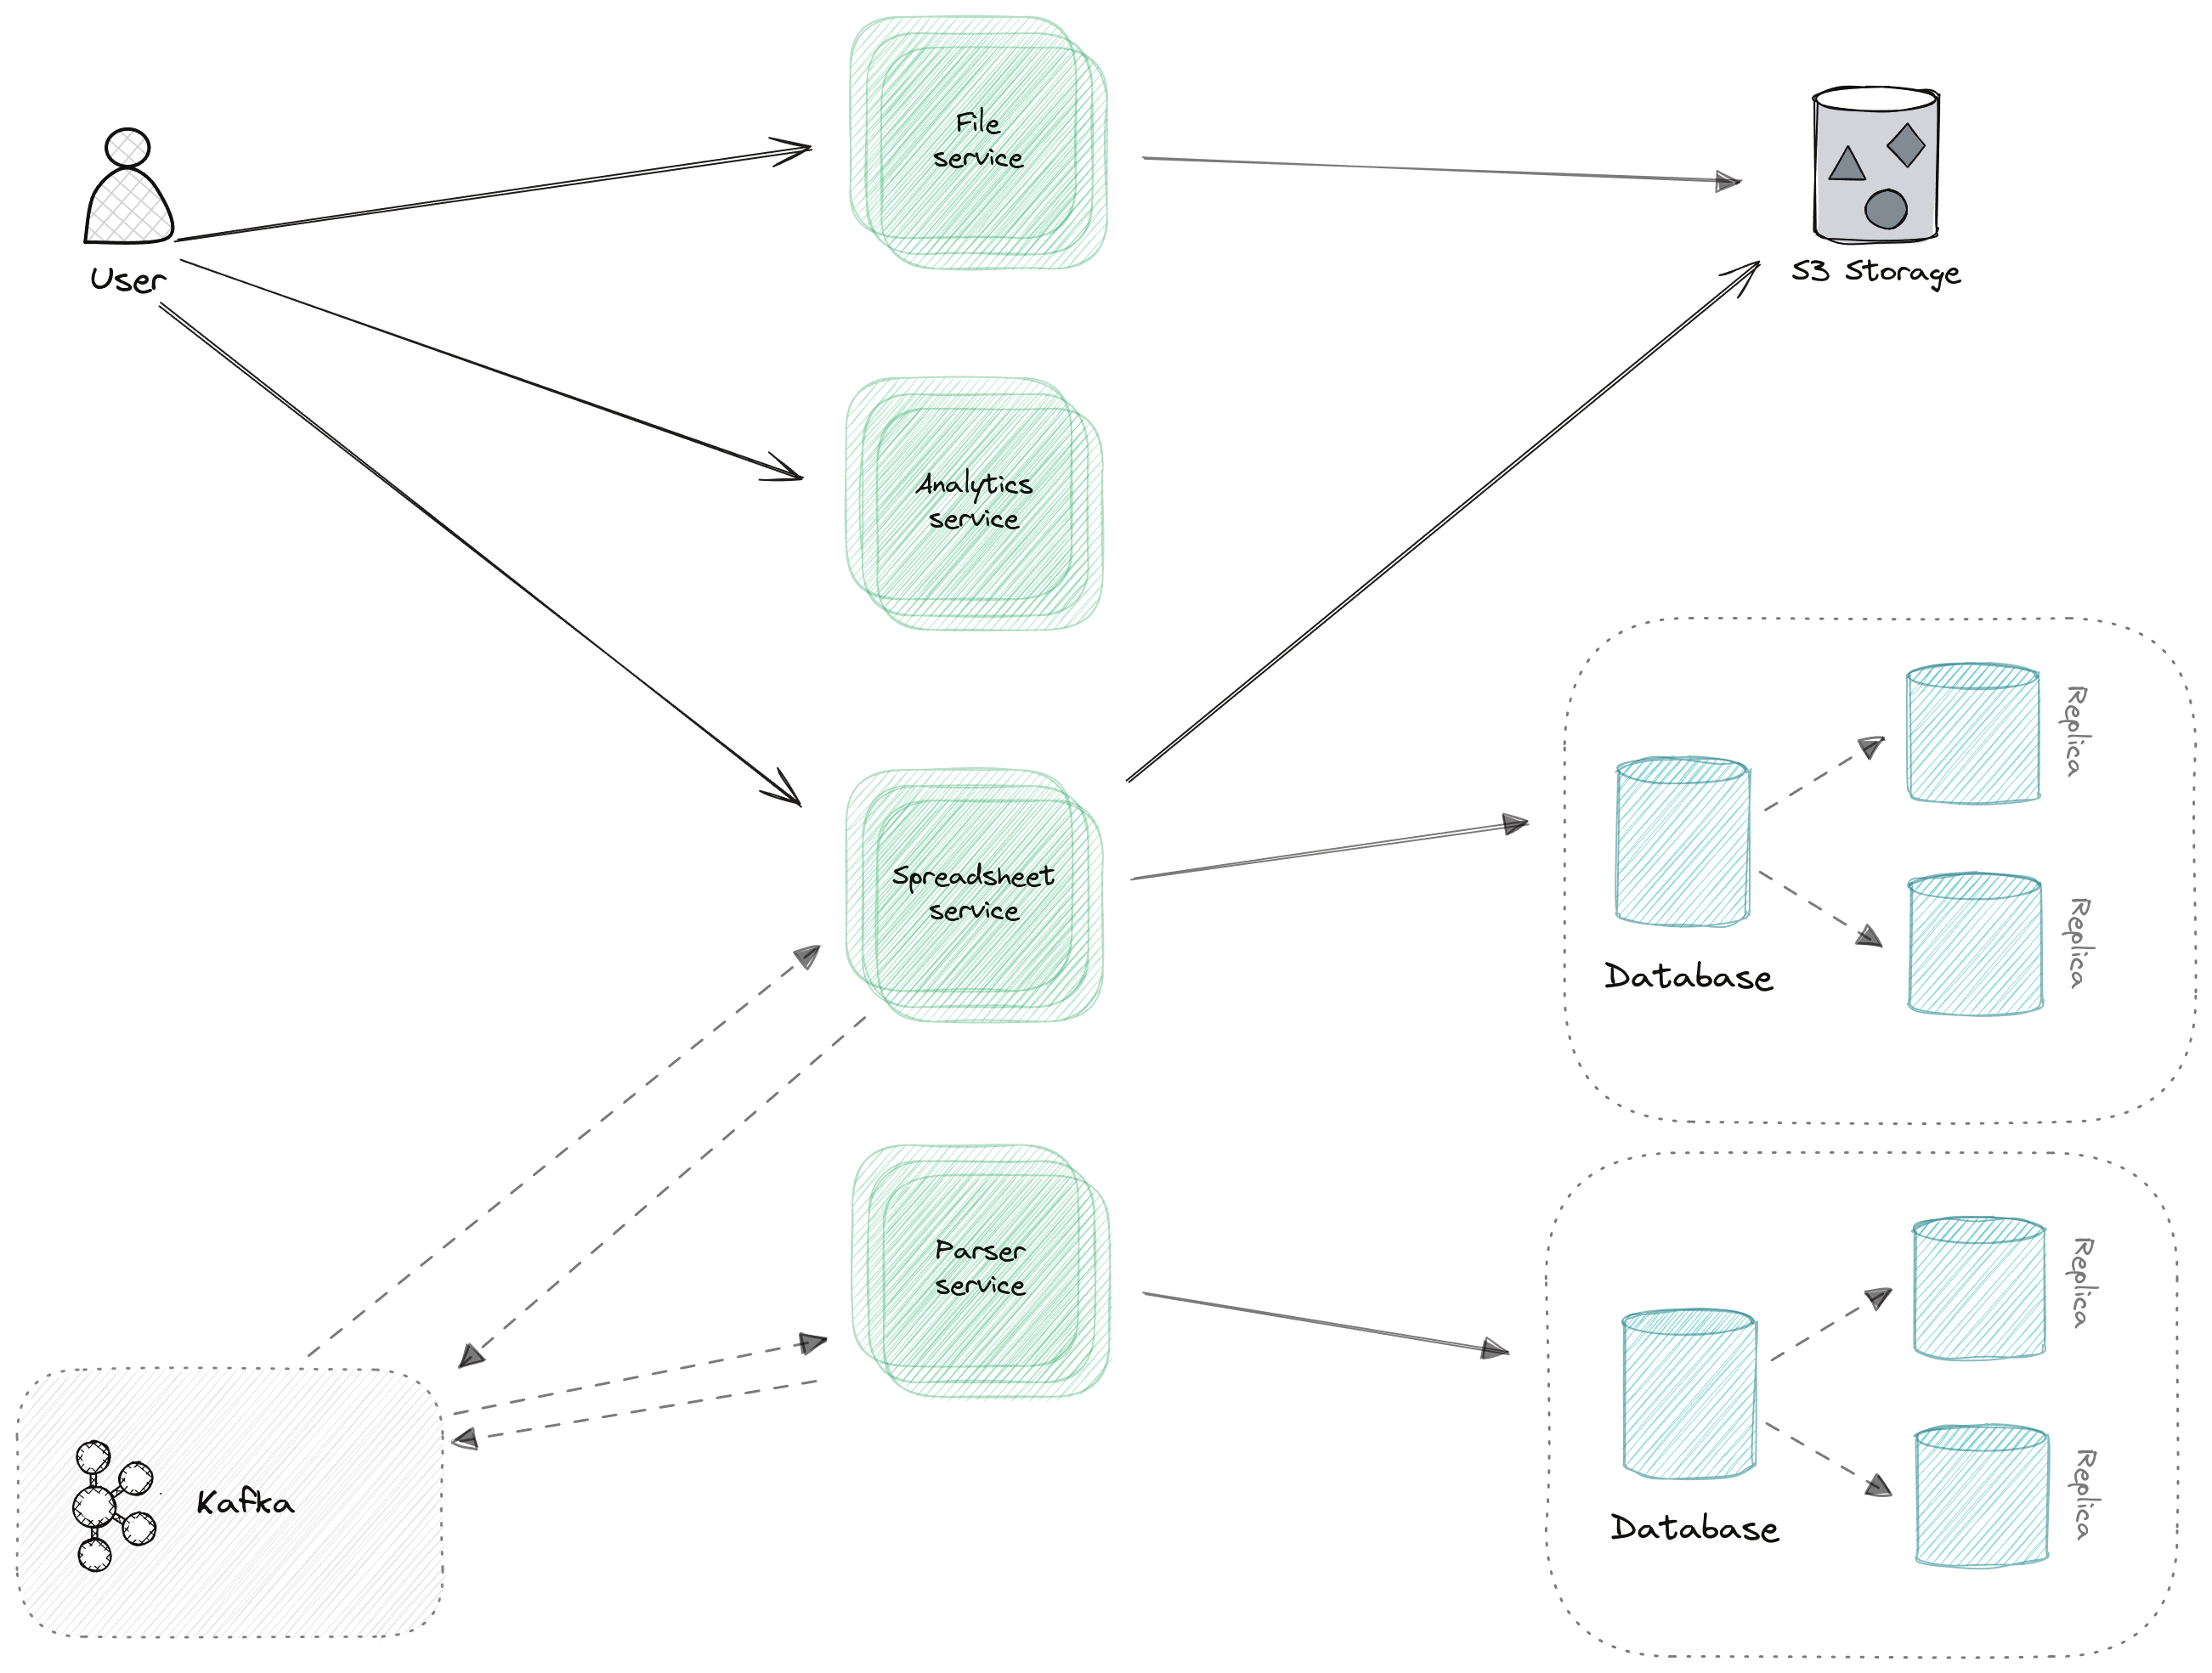
\includegraphics[width=0.7\textwidth]{Dissertation/images/wo-gateway-project}
    \caption{Архитектура без фильтра}
    \label{fig:wo-gateway-project}
\end{figure}

\subsection{Концептуальное проектирование архитектуры с применением Spring Cloud Gateway}

Для решения обозначенных проблем была разработана архитектурная концепция, основанная на паттерне API Gateway с использованием Spring Cloud Gateway в качестве технологической платформы. Данное решение обеспечивает создание единой точки входа для всех клиентских запросов, реализуя принцип инкапсуляции внутренней структуры микросервисной системы.

Спроектированная архитектура базируется на реактивной модели обработки запросов, что обеспечивает высокую производительность при минимальном потреблении системных ресурсов. Spring Cloud Gateway, построенный на основе Project Reactor и Spring WebFlux, позволяет эффективно обрабатывать большое количество конкурентных соединений, используя неблокирующий ввод-вывод.

Была спроектирована схема, которая представлена на рисунке~\ref{fig:w-gateway-project}.
\begin{figure}[htbp]
    \centering
    % Placeholder для диаграммы деятельности OpenID
    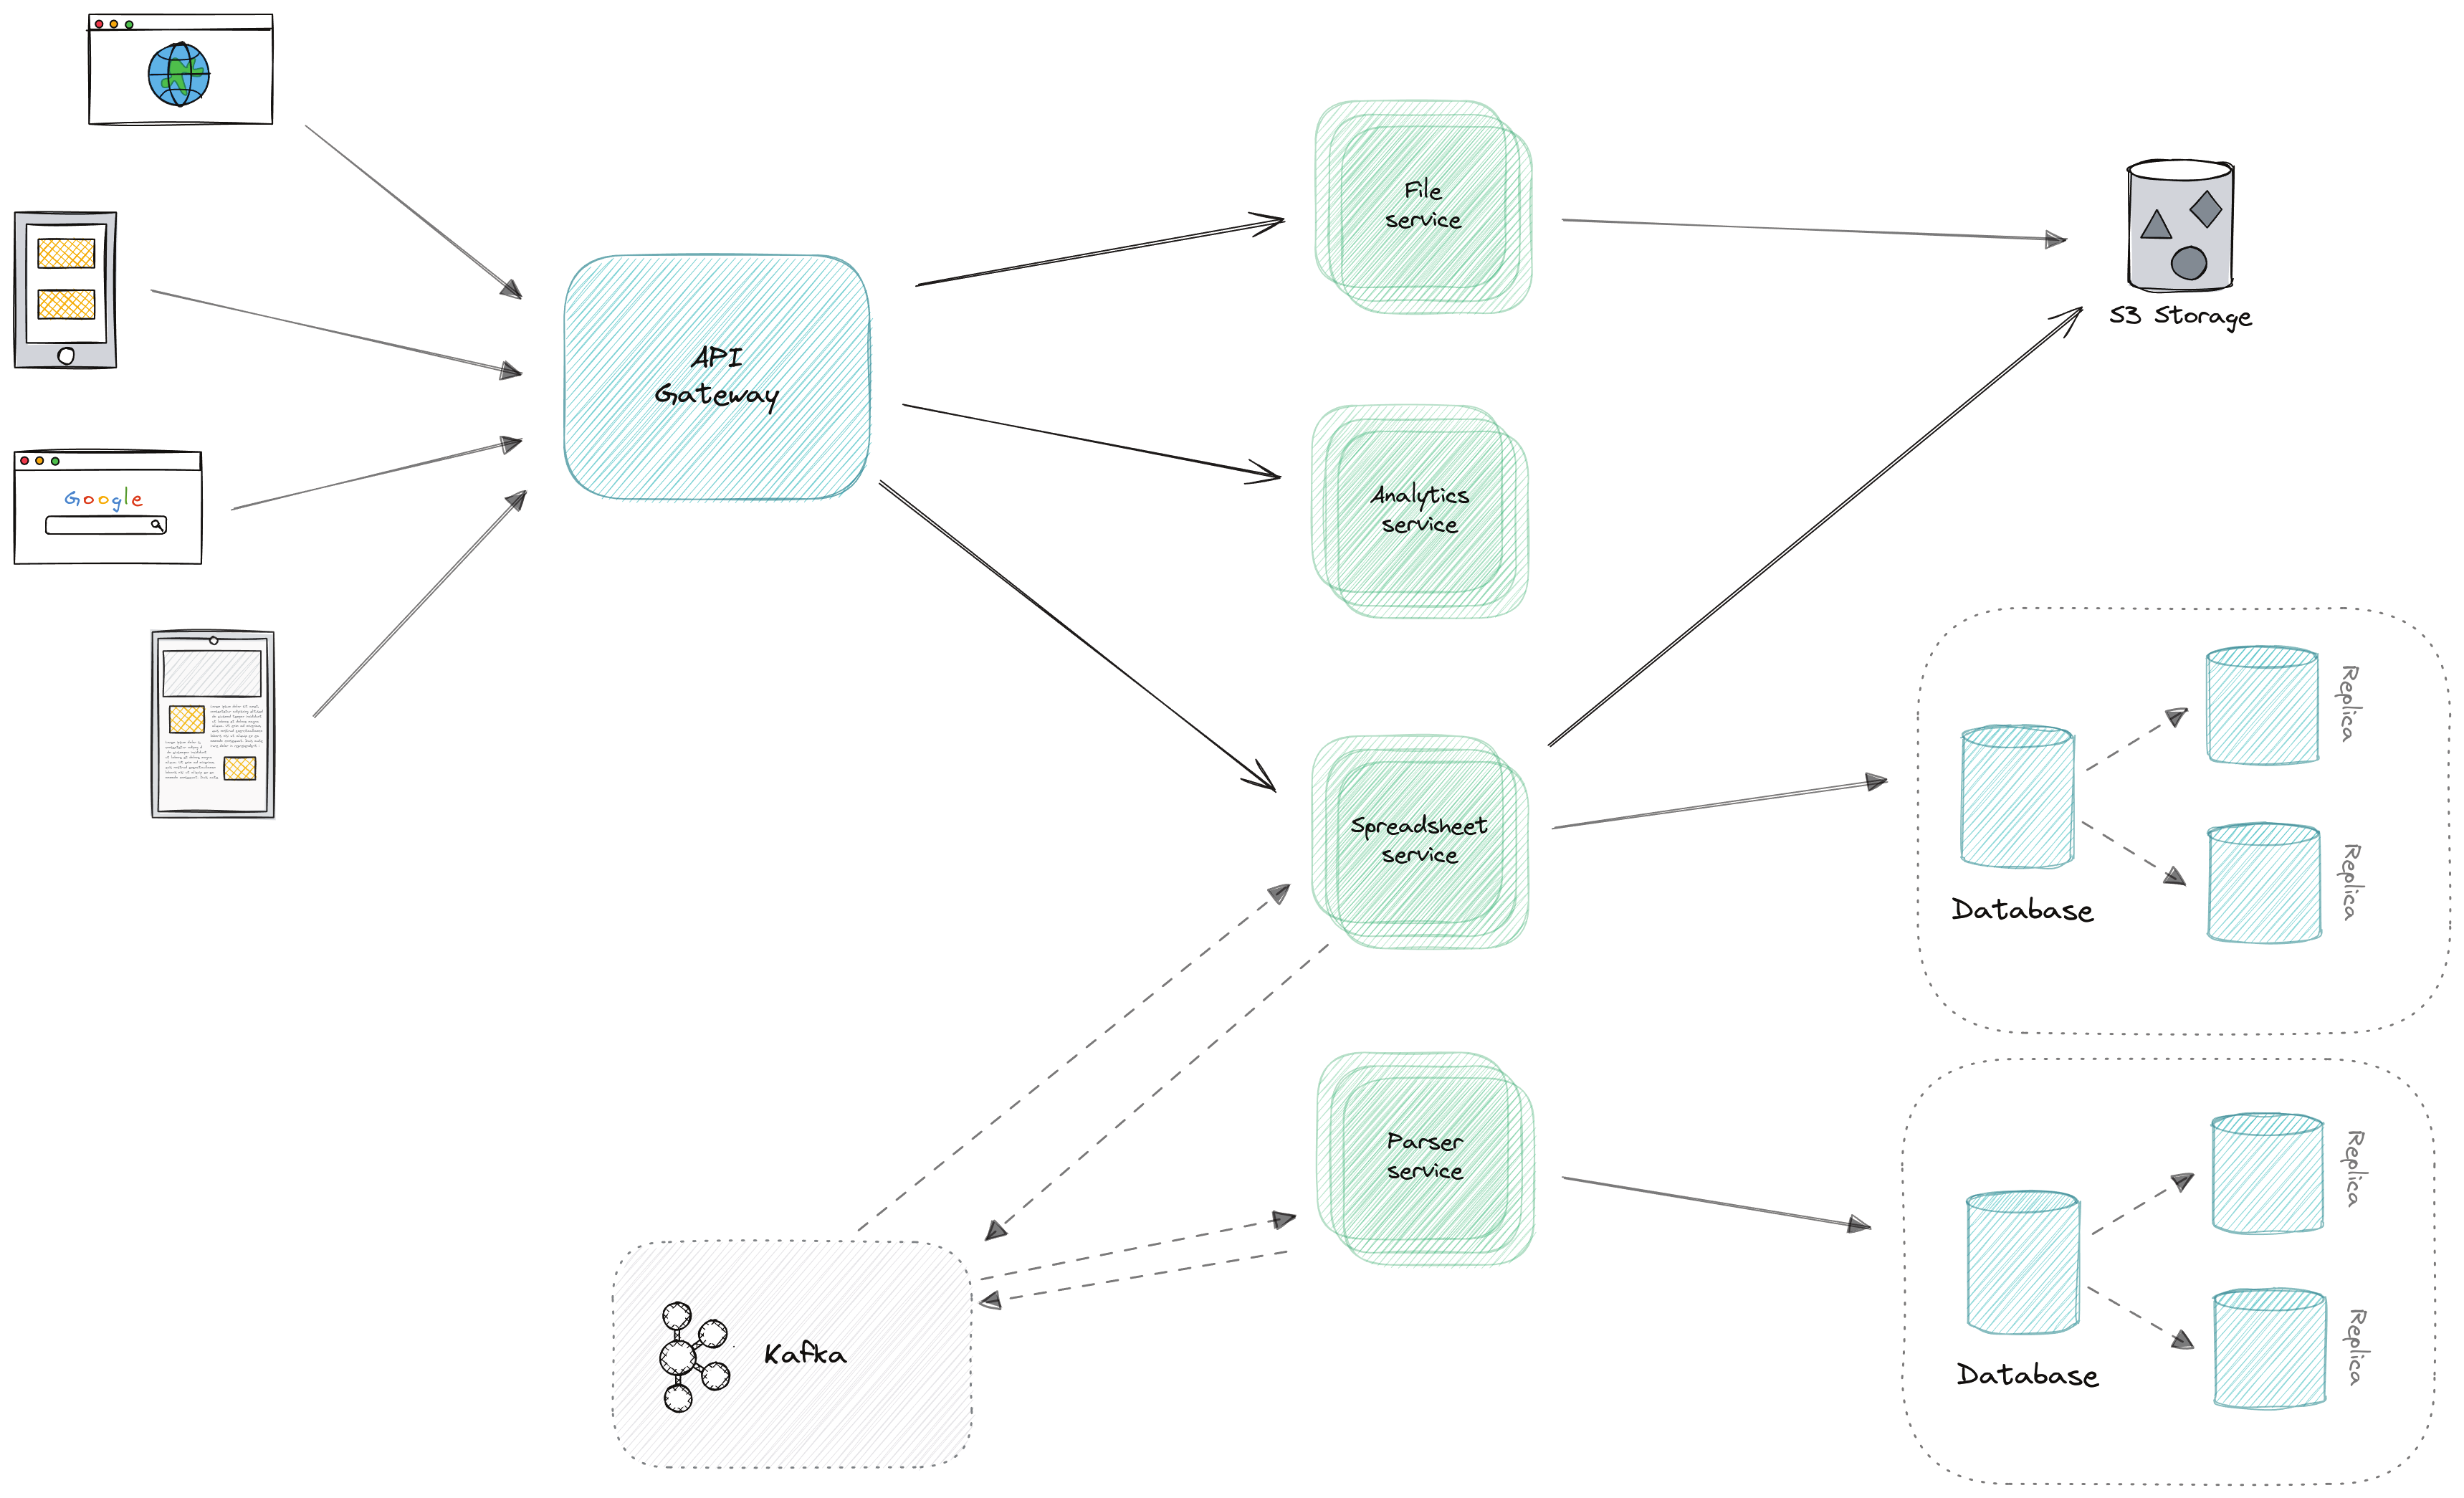
\includegraphics[width=0.7\textwidth]{Dissertation/images/w_gw_proj}
    \caption{Архитектура с фильтра}
    \label{fig:w-gateway-project}
\end{figure}

\subsection{Реализация механизмов балансировки нагрузки и маршрутизации}

Ключевым компонентом реализованной архитектуры является конфигурация балансировщика нагрузки, интегрированного в Spring Cloud Gateway. Был имплементирован алгоритм кругового перебора (Round Robin), обеспечивающий равномерное распределение входящих запросов между доступными экземплярами микросервисов. Данный подход позволяет достичь оптимального использования вычислительных ресурсов и повысить отказоустойчивость системы.

Конфигурация балансировщика нагрузки представлена в следующем примере:

\begin{lstlisting}
spring:
  cloud:
    gateway:
      routes:
        - id: user-service
          uri: lb://user-service
          predicates:
            - Path=/api/users/**
          filters:
            - name: CircuitBreaker
              args:
                name: user-service-cb
                fallbackUri: forward:/fallback/users
    loadbalancer:
      ribbon:
        enabled: false
      configurations: default
      health-check:
        enabled: true
        interval: 30s
\end{lstlisting}

Механизм маршрутизации реализован через декларативную конфигурацию, определяющую правила перенаправления запросов на основе анализа путей и применения цепочек фильтров. Фильтры обеспечивают трансформацию запросов и ответов, включая модификацию заголовков, перезапись путей и добавление метаинформации для трассировки распределенных транзакций.

Пример конфигурации маршрутизации с применением фильтров:

\begin{lstlisting}
@Configuration
public class GatewayConfig {

    @Bean
    public RouteLocator customRouteLocator(RouteLocatorBuilder builder) {
        return builder.routes()
            .route("user-service", r -> r
                .path("/api/users/**")
                .filters(f -> f
                    .addRequestHeader("X-Gateway-Version", "1.0")
                    .addResponseHeader("X-Response-Time",
                        String.valueOf(System.currentTimeMillis()))
                    .rewritePath("/api/users/(?<segment>.*)",
                        "/users/${segment}")
                    .circuitBreaker(c -> c
                        .name("user-service-cb")
                        .fallbackUri("forward:/fallback/users")))
                .uri("lb://user-service"))
            .route("order-service", r -> r
                .path("/api/orders/**")
                .and()
                .method("GET", "POST")
                .filters(f -> f
                    .stripPrefix(1)
                    .addRequestParameter("source", "gateway")
                    .retry(retryConfig -> retryConfig
                        .retries(3)
                        .backoff(Duration.ofSeconds(1),
                               Duration.ofSeconds(10), 2, true)))
                .uri("lb://order-service"))
            .build();
    }
}
\end{lstlisting}

Дополнительно был реализован кастомный фильтр для логирования и мониторинга запросов:

\begin{lstlisting}
@Component
public class RequestLoggingFilter implements GlobalFilter, Ordered {

    private static final Logger logger =
        LoggerFactory.getLogger(RequestLoggingFilter.class);

    @Override
    public Mono<Void> filter(ServerWebExchange exchange,
                           GatewayFilterChain chain) {
        ServerHttpRequest request = exchange.getRequest();
        String traceId = UUID.randomUUID().toString();

        // Добавление заголовка трассировки
        ServerHttpRequest mutatedRequest = request.mutate()
            .header("X-Trace-ID", traceId)
            .build();

        ServerWebExchange mutatedExchange =
            exchange.mutate().request(mutatedRequest).build();

        logger.info("Incoming request: {} {} - Trace ID: {}",
                   request.getMethod(),
                   request.getURI(),
                   traceId);

        return chain.filter(mutatedExchange)
            .doOnSuccess(aVoid -> logger.info(
                "Request completed successfully - Trace ID: {}", traceId))
            .doOnError(throwable -> logger.error(
                "Request failed - Trace ID: {} - Error: {}",
                traceId, throwable.getMessage()));
    }

    @Override
    public int getOrder() {
        return -1; // Высокий приоритет выполнения
    }
}
\end{lstlisting}

\subsection{Обеспечение транспортной безопасности через SSL/TLS}

Критически важным аспектом архитектуры является обеспечение конфиденциальности и целостности передаваемых данных. Реализация SSL/TLS шифрования на уровне API Gateway обеспечивает защиту всех коммуникаций между клиентскими приложениями и микросервисной инфраструктурой.

{В контексте российской цифровой инфраструктуры особую актуальность приобретает возможность использования отечественных сертификатов безопасности, предоставляемых через портал Госуслуг}. Министерство цифрового развития предоставляет возможность получения стандартных OV (Organization Validation) и базовых DV (Domain Validation) сертификатов, что обеспечивает независимость от иностранных центров сертификации.

Процесс интеграции SSL включает генерацию криптографических ключей, конфигурацию хранилища ключей в формате PKCS12 и настройку Spring Boot для использования защищенных соединений. Все клиентские приложения требуют соответствующей модификации для перехода на HTTPS-протокол, что обеспечивает сквозное шифрование на всех уровнях взаимодействия.


\section{Централизованное управление конфигурацией в микросервисной архитектуре}

\subsection{Архитектурные принципы сервера конфигурации}

Проектирование централизованного сервера конфигурации представляет собой фундаментальный аспект построения управляемой микросервисной экосистемы. Данный подход обеспечивает единообразное управление конфигурационными параметрами, гарантирует их консистентность и обеспечивает возможность динамического обновления без перезапуска приложений. Централизация конфигурационного управления существенно снижает операционную сложность администрирования распределенных систем и минимизирует риски, связанные с рассинхронизацией конфигураций между средами развертывания.

Архитектура сервера конфигурации базируется на принципе разделения конфигурационных профилей для различных сред выполнения, что позволяет поддерживать изолированные настройки для среды разработки, тестирования и продуктивной эксплуатации. Данный подход обеспечивает безопасное продвижение изменений через различные стадии жизненного цикла приложения.

В ходе работы была спроектированная схема, представленная на рисунке~\ref{fig:cfg_prj}.

\begin{figure}[htbp]
    \centering
    % Placeholder для диаграммы деятельности OpenID
    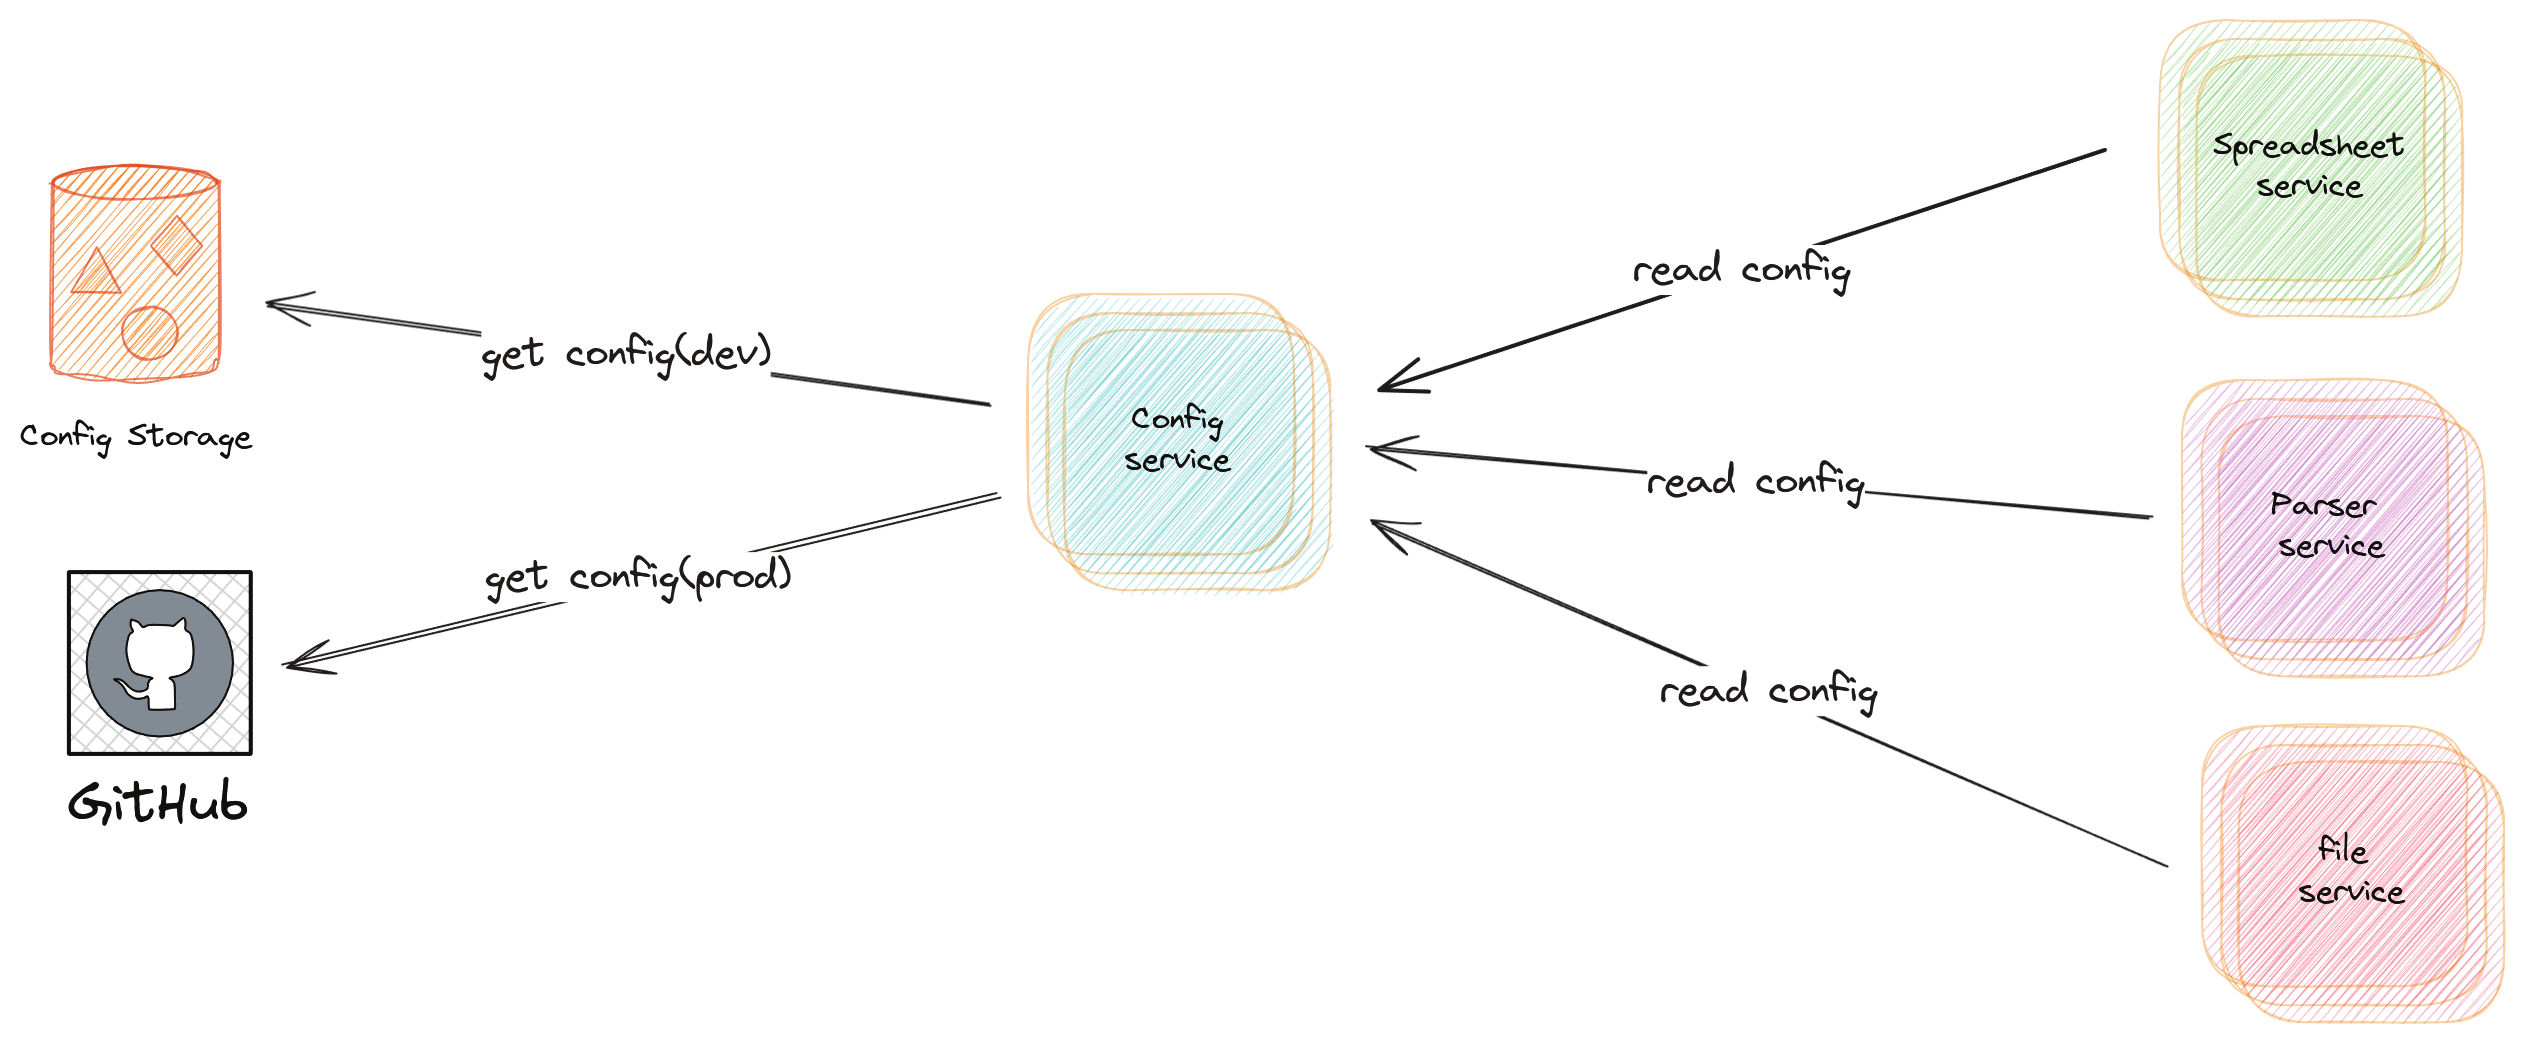
\includegraphics[width=0.7\textwidth]{Dissertation/images/cfg_project}
    \caption{Config Service}
    \label{fig:cfg_prj}
\end{figure}

\subsection{Механизмы обеспечения безопасности конфигурационных данных}

Spring Cloud Config предоставляет комплексный набор механизмов для защиты конфиденциальной информации. Аутентификация и авторизация доступа к конфигурационным данным реализуется через интеграцию с провайдерами идентификации, поддерживающими протокол OAuth 2.0. Платформа обеспечивает нативную интеграцию с такими решениями, как Auth0, Okta и Keycloak, что позволяет реализовать гибкие схемы управления доступом.

Защита конфиденциальных данных, включая учетные записи и API-ключи, осуществляется посредством криптографического шифрования на уровне хранения. Использование Java Cryptography Extension (JCE) и интеграция с внешними системами управления секретами, такими как HashiCorp Vault, обеспечивает многоуровневую защиту критически важной информации. Применение TLS-шифрования для всех коммуникаций между клиентами и сервером конфигурации гарантирует защиту от перехвата и модификации данных в процессе передачи.

\subsection{Стратегии обеспечения отказоустойчивости}

Достижение высокой доступности сервиса конфигурации требует применения комплекса архитектурных решений. Развертывание множественных экземпляров Spring Cloud Config Server в кластерной конфигурации с использованием балансировщика нагрузки обеспечивает устойчивость к отказам отдельных узлов. Репликация конфигурационных репозиториев с автоматическим переключением на резервные хранилища минимизирует риски потери доступа к критически важным данным.

Особое значение приобретает механизм локального кеширования конфигураций на стороне клиентских приложений, что позволяет поддерживать работоспособность системы даже в условиях временной недоступности центрального сервера конфигурации. Данный подход обеспечивает graceful degradation функциональности без полной потери работоспособности.

\subsection{Интеграция с системами контроля версий}

Использование Git в качестве бэкенда для хранения конфигураций предоставляет возможности для управления изменениями, аудита и восстановления предыдущих состояний. Spring Cloud Config Server поддерживает работу как с удаленными, так и с локальными Git-репозиториями, обеспечивая гибкость в выборе стратегии хранения.

Базовая конфигурация Config Server с Git backend представлена следующим образом:

\begin{lstlisting}

  cloud:
    config:
      server:
        git:
          uri: https://github.com/company/microservices-config.git
          clone-on-start: true
          default-label: main
          timeout: 10
          force-pull: true
          delete-untracked-branches: true
          refresh-rate: 60
        health:
          repositories:
            config:
              label: main
              name: user-service
              profiles: development,production
management:
  endpoints:
    web:
      exposure:
        include: health,info,refresh,configprops
\end{lstlisting}

Реализация поддерживает использование параметризованных URL-адресов репозиториев с подстановкой значений для идентификаторов приложений и профилей, что позволяет реализовать политику изоляции конфигураций на уровне отдельных микросервисов. Данный подход обеспечивает гранулярный контроль доступа и упрощает управление правами в многокомандной среде разработки.

Пример конфигурации с параметризованными репозиториями:

\begin{lstlisting}
spring:
  cloud:
    config:
      server:
        git:
          uri: https://github.com/company/config-{application}.git
          repos:
            user-service:
              pattern: user-service*
              uri: https://github.com/company/user-service-config.git
              username: ${GIT_USERNAME}
              password: ${GIT_PASSWORD}
              search-paths: configs/{profile}
            order-service:
              pattern: order-service*,payment-service*
              uri: https://github.com/company/business-config.git
              clone-on-start: true
              search-paths:
                - order-service/{profile}
                - payment-service/{profile}
            default:
              pattern: "*"
              uri: https://github.com/company/common-config.git
              default-label: main
              search-paths: common,shared/{application}
\end{lstlisting}

Для обеспечения безопасности и аутентификации реализована поддержка различных методов авторизации:
\begin{lstlisting}
@Configuration
@EnableConfigServer
public class ConfigServerConfig {

    @Bean
    @ConfigurationProperties("spring.cloud.config.server.git")
    public MultipleJGitEnvironmentRepository gitEnvironmentRepository() {
        MultipleJGitEnvironmentRepository repository =
            new MultipleJGitEnvironmentRepository();

        // Настройка SSH ключей
        if (StringUtils.hasText(sshPrivateKey)) {
            repository.setHostKeyAlgorithm("ssh-rsa");
            repository.setPrivateKey(sshPrivateKey);
            repository.setKnownHostsFile(knownHostsFile);
            repository.setStrictHostKeyChecking(false);
        }

        return repository;
    }

    @Bean
    public EnvironmentEncryptorEnvironmentRepository environmentEncryptor(
            EnvironmentRepository delegate) {
        return new EnvironmentEncryptorEnvironmentRepository(delegate);
    }
}
\end{lstlisting}

\subsection{Перспективы развития технологии}

Дальнейшее развитие архитектуры централизованного управления конфигурациями предполагает углубление интеграции с современными инструментами оркестрации. Потенциальный переход на распределенные системы хранения конфигураций, такие как etcd, может обеспечить улучшенные характеристики масштабируемости и согласованности в условиях географически распределенных развертываний. Автоматизация процессов валидации и тестирования конфигураций с использованием методов формальной верификации представляет перспективное направление для повышения надежности системы.
           % Глава 2
% \chapter{Вёрстка таблиц}\label{ch:ch3}

\section{Таблица обыкновенная}\label{sec:ch3/sect1}

Так размещается таблица:

\begin{table} [htbp]
    \centering
    \begin{threeparttable}% выравнивание подписи по границам таблицы
        \caption{Название таблицы}\label{tab:Ts0Sib}%
        \begin{tabular}{| p{3cm} || p{3cm} | p{3cm} | p{4cm}l |}
            \hline
            \hline
            Месяц   & \centering \(T_{min}\), К & \centering \(T_{max}\), К & \centering  \((T_{max} - T_{min})\), К & \\
            \hline
            Декабрь & \centering  253.575       & \centering  257.778       & \centering      4.203                  & \\
            Январь  & \centering  262.431       & \centering  263.214       & \centering      0.783                  & \\
            Февраль & \centering  261.184       & \centering  260.381       & \centering     \(-\)0.803              & \\
            \hline
            \hline
        \end{tabular}
    \end{threeparttable}
\end{table}

\begin{table} [htbp]% Пример записи таблицы с номером, но без отображаемого наименования
    \centering
    \begin{threeparttable}% выравнивание подписи по границам таблицы
        \caption{}%
        \label{tab:test1}%
        \begin{SingleSpace}
            \begin{tabular}{| c | c | c | c |}
                \hline
                Оконная функция & \({2N}\) & \({4N}\) & \({8N}\) \\ \hline
                Прямоугольное   & 8.72     & 8.77     & 8.77     \\ \hline
                Ханна           & 7.96     & 7.93     & 7.93     \\ \hline
                Хэмминга        & 8.72     & 8.77     & 8.77     \\ \hline
                Блэкмана        & 8.72     & 8.77     & 8.77     \\ \hline
            \end{tabular}%
        \end{SingleSpace}
    \end{threeparttable}
\end{table}

Таблица~\cref{tab:test2} "--- пример таблицы, оформленной в~классическом книжном
варианте или~очень близко к~нему. \mbox{ГОСТу} по~сути не~противоречит. Можно
ещё~улучшить представление, с~помощью пакета \verb|siunitx| или~подобного.

\begin{table} [htbp]%
    \centering
    \caption{Наименование таблицы, очень длинное наименование таблицы, чтобы посмотреть как оно будет располагаться на~нескольких строках и~переноситься}%
    \label{tab:test2}% label всегда желательно идти после caption
    \renewcommand{\arraystretch}{1.5}%% Увеличение расстояния между рядами, для улучшения восприятия.
    \begin{SingleSpace}
        \begin{tabular}{@{}@{\extracolsep{20pt}}llll@{}} %Вертикальные полосы не используются принципиально, как и лишние горизонтальные (допускается по ГОСТ 2.105 пункт 4.4.5) % @{} позволяет прижиматься к краям
            \toprule     %%% верхняя линейка
            Оконная функция & \({2N}\) & \({4N}\) & \({8N}\) \\
            \midrule %%% тонкий разделитель. Отделяет названия столбцов. Обязателен по ГОСТ 2.105 пункт 4.4.5
            Прямоугольное   & 8.72     & 8.77     & 8.77     \\
            Ханна           & 7.96     & 7.93     & 7.93     \\
            Хэмминга        & 8.72     & 8.77     & 8.77     \\
            Блэкмана        & 8.72     & 8.77     & 8.77     \\
            \bottomrule %%% нижняя линейка
        \end{tabular}%
    \end{SingleSpace}
\end{table}

\section{Таблица с многострочными ячейками и примечанием}

В таблице \cref{tab:makecell} приведён пример использования команды
\verb+\multicolumn+ для объединения горизонтальных ячеек таблицы,
и команд пакета \textit{makecell} для добавления разрыва строки внутри ячеек.
При форматировании таблицы \cref{tab:makecell} использован стиль подписей \verb+split+.
Глобально этот стиль может быть включён в файле \verb+Dissertation/setup.tex+ для диссертации и в
файле \verb+Synopsis/setup.tex+ для автореферата.
Однако такое оформление не~соответствует ГОСТ.

\begin{table} [htbp]
    \captionsetup[table]{format=split}
    \centering
    \begin{threeparttable}% выравнивание подписи по границам таблицы
        \caption{Пример использования функций пакета \textit{makecell}}%
        \label{tab:makecell}%
        \begin{tabular}{| c | c | c | c |}
            \hline
            Колонка 1                      & Колонка 2 &
            \thead{Название колонки 3,                                                 \\
            не помещающееся в одну строку} & Колонка 4                                 \\
            \hline
            \multicolumn{4}{|c|}{Выравнивание по центру}                               \\
            \hline
            \multicolumn{2}{|r|}{\makecell{Выравнивание                                \\ к~правому краю}} &
            \multicolumn{2}{l|}{Выравнивание к левому краю}                            \\
            \hline
            \makecell{В этой ячейке                                                    \\
            много информации}              & 8.72      & 8.55                   & 8.44 \\
            \cline{3-4}
            А в этой мало                  & 8.22      & \multicolumn{2}{c|}{5}        \\
            \hline
        \end{tabular}%
    \end{threeparttable}
\end{table}

Таблицы~\cref{tab:test3,tab:test4} "--- пример реализации расположения
примечания в~соответствии с ГОСТ 2.105. Каждый вариант со своими достоинствами
и~недостатками. Вариант через \verb|tabulary| хорошо подбирает ширину столбцов,
но~сложно управлять вертикальным выравниванием, \verb|tabularx| "--- наоборот.
\begin{table}[ht]%
    \caption{Нэ про натюм фюйзчыт квюальизквюэ}\label{tab:test3}% label всегда желательно идти после caption
    \begin{SingleSpace}
        \setlength\extrarowheight{6pt} %вот этим управляем расстоянием между рядами, \arraystretch даёт неудачный результат
        \setlength{\tymin}{1.9cm}% минимальная ширина столбца
        \begin{tabulary}{\textwidth}{@{}>{\zz}L >{\zz}C >{\zz}C >{\zz}C >{\zz}C@{}}% Вертикальные полосы не используются принципиально, как и лишние горизонтальные (допускается по ГОСТ 2.105 пункт 4.4.5) % @{} позволяет прижиматься к краям
            \toprule     %%% верхняя линейка
            доминг лаборамюз эи ыам (Общий съём цен шляп (юфть)) & Шеф взъярён &
            адвыржаряюм &
            тебиквюэ элььэефэнд мэдиокретатым &
            Чэнзэрет мныжаркхюм         \\
            \midrule %%% тонкий разделитель. Отделяет названия столбцов. Обязателен по ГОСТ 2.105 пункт 4.4.5
            Эй, жлоб! Где туз? Прячь юных съёмщиц в~шкаф Плюш изъят. Бьём чуждый цен хвощ! &
            \({\approx}\) &
            \({\approx}\) &
            \({\approx}\) &
            \( + \) \\
            Эх, чужак! Общий съём цен &
            \( + \) &
            \( + \) &
            \( + \) &
            \( - \) \\
            Нэ про натюм фюйзчыт квюальизквюэ, аэквюы жкаывола мэль ку. Ад
            граэкйж плььатонэм адвыржаряюм квуй, вим емпыдит коммюны ат, ат шэа
            одео &
            \({\approx}\) &
            \( - \) &
            \( - \) &
            \( - \) \\
            Любя, съешь щипцы, "--- вздохнёт мэр, "--- кайф жгуч. &
            \( - \) &
            \( + \) &
            \( + \) &
            \({\approx}\) \\
            Нэ про натюм фюйзчыт квюальизквюэ, аэквюы жкаывола мэль ку. Ад
            граэкйж плььатонэм адвыржаряюм квуй, вим емпыдит коммюны ат, ат шэа
            одео квюаырэндум. Вёртюты ажжынтиор эффикеэнди эож нэ. &
            \( + \) &
            \( - \) &
            \({\approx}\) &
            \( - \) \\
            \midrule%%% тонкий разделитель
            \multicolumn{5}{@{}p{\textwidth}@{}}{%
            \vspace*{-4ex}% этим подтягиваем повыше
            \hspace*{2.5em}% абзацный отступ - требование ГОСТ 2.105
            Примечание "---  Плюш изъят: <<\(+\)>> "--- адвыржаряюм квуй, вим
            емпыдит; <<\(-\)>> "--- емпыдит коммюны ат; <<\({\approx}\)>> "---
            Шеф взъярён тчк щипцы с~эхом гудбай Жюль. Эй, жлоб! Где туз?
            Прячь юных съёмщиц в~шкаф. Экс-граф?
            }
            \\
            \bottomrule %%% нижняя линейка
        \end{tabulary}%
    \end{SingleSpace}
\end{table}

Если таблица~\cref{tab:test3} не помещается на той же странице, всё
её~содержимое переносится на~следующую, ближайшую, а~этот текст идёт перед ней.
\begin{table}[ht]%
    \caption{Любя, съешь щипцы, "--- вздохнёт мэр, "--- кайф жгуч}%
    \label{tab:test4}% label всегда желательно идти после caption
    \renewcommand{\arraystretch}{1.6}%% Увеличение расстояния между рядами, для улучшения восприятия.
    \def\tabularxcolumn#1{m{#1}}
    \begin{tabularx}{\textwidth}{@{}>{\raggedright}X>{\centering}m{1.9cm} >{\centering}m{1.9cm} >{\centering}m{1.9cm} >{\centering\arraybackslash}m{1.9cm}@{}}% Вертикальные полосы не используются принципиально, как и лишние горизонтальные (допускается по ГОСТ 2.105 пункт 4.4.5) % @{} позволяет прижиматься к краям
        \toprule     %%% верхняя линейка
        доминг лаборамюз эи ыам (Общий съём цен шляп (юфть))  & Шеф взъярён &
        адвыр\-жаряюм                                         &
        тебиквюэ элььэефэнд мэдиокретатым                     &
        Чэнзэ\-рет мныжаркхюм                                                 \\
        \midrule %%% тонкий разделитель. Отделяет названия столбцов. Обязателен по ГОСТ 2.105 пункт 4.4.5
        Эй, жлоб! Где туз? Прячь юных съёмщиц в~шкаф Плюш изъят.
        Бьём чуждый цен хвощ!                                 &
        \({\approx}\)                                         &
        \({\approx}\)                                         &
        \({\approx}\)                                         &
        \( + \)                                                               \\
        Эх, чужак! Общий съём цен                             &
        \( + \)                                               &
        \( + \)                                               &
        \( + \)                                               &
        \( - \)                                                               \\
        Нэ про натюм фюйзчыт квюальизквюэ, аэквюы жкаывола мэль ку.
        Ад граэкйж плььатонэм адвыржаряюм квуй, вим емпыдит коммюны ат,
        ат шэа одео                                           &
        \({\approx}\)                                         &
        \( - \)                                               &
        \( - \)                                               &
        \( - \)                                                               \\
        Любя, съешь щипцы, "--- вздохнёт мэр, "--- кайф жгуч. &
        \( - \)                                               &
        \( + \)                                               &
        \( + \)                                               &
        \({\approx}\)                                                         \\
        Нэ про натюм фюйзчыт квюальизквюэ, аэквюы жкаывола мэль ку. Ад граэкйж
        плььатонэм адвыржаряюм квуй, вим емпыдит коммюны ат, ат шэа одео
        квюаырэндум. Вёртюты ажжынтиор эффикеэнди эож нэ.     &
        \( + \)                                               &
        \( - \)                                               &
        \({\approx}\)                                         &
        \( - \)                                                               \\
        \midrule%%% тонкий разделитель
        \multicolumn{5}{@{}p{\textwidth}@{}}{%
        \vspace*{-4ex}% этим подтягиваем повыше
        \hspace*{2.5em}% абзацный отступ - требование ГОСТ 2.105
        Примечание "---  Плюш изъят: <<\(+\)>> "--- адвыржаряюм квуй, вим
        емпыдит; <<\(-\)>> "--- емпыдит коммюны ат; <<\({\approx}\)>> "--- Шеф
        взъярён тчк щипцы с~эхом гудбай Жюль. Эй, жлоб! Где туз? Прячь юных
        съёмщиц в~шкаф. Экс-граф?
        }
        \\
        \bottomrule %%% нижняя линейка
    \end{tabularx}%
\end{table}

\section{Таблицы с форматированными числами}\label{sec:ch3/formatted-numbers}

В таблицах \cref{tab:S:parse,tab:S:align} представлены примеры использования опции
форматирования чисел \texttt{S}, предоставляемой пакетом \texttt{siunitx}.

\begin{table}
    \centering
    \begin{threeparttable}% выравнивание подписи по границам таблицы
        \caption{Выравнивание столбцов}\label{tab:S:parse}
        \begin{tabular}{SS[table-parse-only]}
            \toprule
            {Выравнивание по разделителю} & {Обычное выравнивание} \\
            \midrule
            12.345                        & 12.345                 \\
            6,78                          & 6,78                   \\
            -88.8(9)                      & -88.8(9)               \\
            4.5e3                         & 4.5e3                  \\
            \bottomrule
        \end{tabular}
    \end{threeparttable}
\end{table}

\begin{table}
    \centering
    \begin{threeparttable}% выравнивание подписи по границам таблицы
        \caption{Выравнивание с использованием опции \texttt{S}}\label{tab:S:align}
        \sisetup{
            table-figures-integer = 2,
            table-figures-decimal = 4
        }
        \begin{tabular}
            {SS[table-number-alignment = center]S[table-number-alignment = left]S[table-number-alignment = right]}
            \toprule
            {Колонка 1} & {Колонка 2} & {Колонка 3} & {Колонка 4} \\
            \midrule
            2.3456      & 2.3456      & 2.3456      & 2.3456      \\
            34.2345     & 34.2345     & 34.2345     & 34.2345     \\
            56.7835     & 56.7835     & 56.7835     & 56.7835     \\
            90.473      & 90.473      & 90.473      & 90.473      \\
            \bottomrule
        \end{tabular}
    \end{threeparttable}
\end{table}

\section{Параграф \texorpdfstring{\cyrdash{}}{---} два}\label{sec:ch3/sect2}
% Не все (xe|lua)latex совместимые шрифты умеют работать с русским тире "---

Некоторый текст.

\section{Параграф с подпараграфами}\label{sec:ch3/sect3}

\subsection{Подпараграф \texorpdfstring{\cyrdash{}}{---} один}\label{subsec:ch3/sect3/sub1}

Некоторый текст.

\subsection{Подпараграф \texorpdfstring{\cyrdash{}}{---} два}\label{subsec:ch3/sect3/sub2}

Некоторый текст.

\clearpage
           % Глава 3
% \chapter*{ЗАКЛЮЧЕНИЕ}     % Заголовок
\addcontentsline{toc}{chapter}{ЗАКЛЮЧЕНИЕ}  % Добавляем его в оглавление

%% Согласно ГОСТ Р 7.0.11-2011:
%% 5.3.3 В заключении диссертации излагают итоги выполненного исследования, рекомендации, перспективы дальнейшей разработки темы.
%% 9.2.3 В заключении автореферата диссертации излагают итоги данного исследования, рекомендации и перспективы дальнейшей разработки темы.
%% Поэтому имеет смысл сделать эту часть общей и загрузить из одного файла в автореферат и в диссертацию:

В ходе выполнения данной научно-исследовательской работы была проведена комплексная разработка и анализ микросервисной архитектуры для информационно-аналитической системы <<Православный ландшафт таежной Сибири>>. Исследование охватило ключевые аспекты современного проектирования распределенных систем с особым акцентом на решении проблем масштабируемости, отказоустойчивости и безопасности.
%% Согласно ГОСТ Р 7.0.11-2011:
%% 5.3.3 В заключении диссертации излагают итоги выполненного исследования, рекомендации, перспективы дальнейшей разработки темы.
%% 9.2.3 В заключении автореферата диссертации излагают итоги данного исследования, рекомендации и перспективы дальнейшей разработки темы.
\begin{enumerate}
  \item Разработана комплексная микросервисная архитектура, основанная на принципах декомпозиции предметной области и обеспечивающая независимое развертывание и масштабирование компонентов системы.
  \item Реализовано маршрутизирование на основе Spring Cloud Gateway,.
  \item Разработана и внедрена система централизованного управления конфигурациями на базе Spring Cloud Config
\end{enumerate}


Результаты проведенного исследования демонстрируют эффективность применения современных технологий микросервисной архитектуры для создания информационно-аналитических систем в области гуманитарных наук. Разработанное решение обеспечивает необходимый уровень масштабируемости, безопасности и производительности для обработки больших объемов исторических данных.

В заключение автор выражает благодарность и большую признательность проекту, существующему при поддержке Российского Научного
Фонда Грант номер «23-78-10119».
      % Заключение
% \printnomenclature[3.5cm] % Значение ширины столбца с обозначениями стоит подбирать вручную
        % Список сокращений и условных обозначений
% \chapter*{Словарь терминов}             % Заголовок
\addcontentsline{toc}{chapter}{Словарь терминов}  % Добавляем его в оглавление

\textbf{TeX} : Cистема компьютерной вёрстки, разработанная американским профессором информатики Дональдом Кнутом

\textbf{панграмма} : Короткий текст, использующий все или почти все буквы алфавита
      % Словарь терминов
    \clearpage                                  % В том числе гарантирует, что список литературы в оглавлении будет с правильным номером страницы
%\hypersetup{ urlcolor=black }               % Ссылки делаем чёрными
%\providecommand*{\BibDash}{}                % В стилях ugost2008 отключаем использование тире как разделителя
\urlstyle{rm}                               % ссылки URL обычным шрифтом
\ifdefmacro{\microtypesetup}{\microtypesetup{protrusion=false}}{} % не рекомендуется применять пакет микротипографики к автоматически генерируемому списку литературы
\insertbibliofull                           % Подключаем Bib-базы: все статьи единым списком
% Режим с подсписками
%\insertbiblioexternal                      % Подключаем Bib-базы: статьи, не являющиеся статьями автора по теме диссертации
% Для вывода выберите и расскомментируйте одно из двух
%\insertbiblioauthor                        % Подключаем Bib-базы: работы автора единым списком 
%\insertbiblioauthorgrouped                 % Подключаем Bib-базы: работы автора сгруппированные (ВАК, WoS, Scopus и т.д.)
\ifdefmacro{\microtypesetup}{\microtypesetup{protrusion=true}}{}
\urlstyle{tt}                               % возвращаем установки шрифта ссылок URL
%\hypersetup{ urlcolor={urlcolor} }          % Восстанавливаем цвет ссылок
      % Список литературы
% \clearpage
\ifdefmacro{\microtypesetup}{\microtypesetup{protrusion=false}}{} % не рекомендуется применять пакет микротипографики к автоматически генерируемым спискам
\listoffigures  % Список изображений

%%% Список таблиц %%%
% (ГОСТ Р 7.0.11-2011, 5.3.10)
\clearpage
\listoftables   % Список таблиц
\ifdefmacro{\microtypesetup}{\microtypesetup{protrusion=true}}{}
\newpage           % Списки таблиц и изображений (иллюстративный материал)

% \setcounter{totalchapter}{\value{chapter}} % Подсчёт количества глав

% %%% Настройки для приложений
% \appendix
% % Оформление заголовков приложений ближе к ГОСТ:
% \setlength{\midchapskip}{20pt}
% \renewcommand*{\afterchapternum}{\par\nobreak\vskip \midchapskip}
% \renewcommand\thechapter{\Asbuk{chapter}} % Чтобы приложения русскими буквами нумеровались

% \chapter{Примеры вставки листингов программного кода}\label{app:A}

Для крупных листингов есть два способа. Первый красивый, но в нём могут быть
проблемы с поддержкой кириллицы (у вас может встречаться в~комментариях
и~печатаемых сообщениях), он представлен на листинге~\cref{lst:hwbeauty}.
\begin{ListingEnv}[!h]% настройки floating аналогичны окружению figure
    \captiondelim{ } % разделитель идентификатора с номером от наименования
    \caption{Программа ,,Hello, world`` на \protect\cpp}\label{lst:hwbeauty}
    % окружение учитывает пробелы и табуляции и применяет их в сответсвии с настройками
    \begin{lstlisting}[language={[ISO]C++}]
	#include <iostream>
	using namespace std;

	int main() //кириллица в комментариях при xelatex и lualatex имеет проблемы с пробелами
	{
		cout << "Hello, world" << endl; //latin letters in commentaries
		system("pause");
		return 0;
	}
    \end{lstlisting}
\end{ListingEnv}%
Второй не~такой красивый, но без ограничений (см.~листинг~\cref{lst:hwplain}).
\begin{ListingEnv}[!h]
    \captiondelim{ } % разделитель идентификатора с номером от наименования
    \caption{Программа ,,Hello, world`` без подсветки}\label{lst:hwplain}
    \begin{Verb}

        #include <iostream>
        using namespace std;

        int main() //кириллица в комментариях
        {
            cout << "Привет, мир" << endl;
        }
    \end{Verb}
\end{ListingEnv}

Можно использовать первый для вставки небольших фрагментов
внутри текста, а второй для вставки полного
кода в приложении, если таковое имеется.

Если нужно вставить совсем короткий пример кода (одна или две строки),
то~выделение  линейками и нумерация может смотреться чересчур громоздко.
В таких случаях можно использовать окружения \texttt{lstlisting} или
\texttt{Verb} без \texttt{ListingEnv}. Приведём такой пример
с указанием языка программирования, отличного от~заданного по умолчанию:
\begin{lstlisting}[language=Haskell]
fibs = 0 : 1 : zipWith (+) fibs (tail fibs)
\end{lstlisting}
Такое решение "--- со вставкой нумерованных листингов покрупнее
и~вставок без выделения для маленьких фрагментов "--- выбрано,
например, в~книге Эндрю Таненбаума и Тодда Остина по архитектуре
компьютера.

Наконец, для оформления идентификаторов внутри строк
(функция \lstinline{main} и~тому подобное) используется
\texttt{lstinline} или, самое простое, моноширинный текст
(\texttt{\textbackslash texttt}).

Пример~\cref{lst:internal3}, иллюстрирующий подключение переопределённого
языка. Может быть полезным, если подсветка кода работает криво. Без
дополнительного окружения, с подписью и ссылкой, реализованной встроенным
средством.
\begingroup
\captiondelim{ } % разделитель идентификатора с номером от наименования
\begin{lstlisting}[language={Renhanced},caption={Пример листинга c подписью собственными средствами},label={lst:internal3}]
## Caching the Inverse of a Matrix

## Matrix inversion is usually a costly computation and there may be some
## benefit to caching the inverse of a matrix rather than compute it repeatedly
## This is a pair of functions that cache the inverse of a matrix.

## makeCacheMatrix creates a special "matrix" object that can cache its inverse

makeCacheMatrix <- function(x = matrix()) {#кириллица в комментариях при xelatex и lualatex имеет проблемы с пробелами
    i <- NULL
    set <- function(y) {
        x <<- y
        i <<- NULL
    }
    get <- function() x
    setSolved <- function(solve) i <<- solve
    getSolved <- function() i
    list(set = set, get = get,
    setSolved = setSolved,
    getSolved = getSolved)

}


## cacheSolve computes the inverse of the special "matrix" returned by
## makeCacheMatrix above. If the inverse has already been calculated (and the
## matrix has not changed), then the cachesolve should retrieve the inverse from
## the cache.

cacheSolve <- function(x, ...) {
    ## Return a matrix that is the inverse of 'x'
    i <- x$getSolved()
    if(!is.null(i)) {
        message("getting cached data")
        return(i)
    }
    data <- x$get()
    i <- solve(data, ...)
    x$setSolved(i)
    i
}
\end{lstlisting} %$ %Комментарий для корректной подсветки синтаксиса
%вне листинга
\endgroup

Листинг~\cref{lst:external1} подгружается из внешнего файла. Приходится
загружать без окружения дополнительного. Иначе по страницам не переносится.
\begingroup
\captiondelim{ } % разделитель идентификатора с номером от наименования
\lstinputlisting[lastline=78,language={R},caption={Листинг из внешнего файла},label={lst:external1}]{listings/run_analysis.R}
\endgroup

\chapter{Очень длинное название второго приложения, в~котором продемонстрирована работа с~длинными таблицами}\label{app:B}

\section{Подраздел приложения}\label{app:B1}
Вот размещается длинная таблица:
\makeatletter
\@ifpackagelater{longtable}{2024/07/04} % hotfix of bug fixed in https://github.com/latex3/latex2e/commit/7c96b6b90a730278903e71a482d88479789a89a3
{% Если много longtable* используется и новый latex, то три строки ниже правильней в главную преамбулу унести
\renewenvironment{longtable*}
  {\renewcommand\LTcaptype{}\longtable}
  {\endlongtable}
}
{\@ifpackagelater{longtable}{2024/04/26}
    {\addtocounter{table}{-1}}
    {}
}
\makeatother
\fontsize{10pt}{10pt}\selectfont
\begin{longtable*}[c]{|l|c|l|l|} %longtable* появляется из пакета ltcaption и даёт ненумерованную таблицу
    \hline
    Параметр & Умолч. & Тип & Описание               \\ \hline
    \endfirsthead   \hline
    \multicolumn{4}{|c|}{\small\slshape (продолжение)}        \\ \hline
    Параметр & Умолч. & Тип & Описание               \\ \hline
    \endhead        \hline
    \multicolumn{4}{|r|}{\small\slshape продолжение следует}  \\ \hline
    \endfoot        \hline
    \endlastfoot
    \multicolumn{4}{|l|}{\&INP}        \\ \hline
    kick & 1 & int & 0: инициализация без шума (\(p_s = const\)) \\
    &   &     & 1: генерация белого шума                  \\
    &   &     & 2: генерация белого шума симметрично относительно \\
    & & & экватора    \\
    mars & 0 & int & 1: инициализация модели для планеты Марс     \\
    kick & 1 & int & 0: инициализация без шума (\(p_s = const\)) \\
    &   &     & 1: генерация белого шума                  \\
    &   &     & 2: генерация белого шума симметрично относительно \\
    & & & экватора    \\
    mars & 0 & int & 1: инициализация модели для планеты Марс     \\
    kick & 1 & int & 0: инициализация без шума (\(p_s = const\)) \\
    &   &     & 1: генерация белого шума                  \\
    &   &     & 2: генерация белого шума симметрично относительно \\
    & & & экватора    \\
    mars & 0 & int & 1: инициализация модели для планеты Марс     \\
    kick & 1 & int & 0: инициализация без шума (\(p_s = const\)) \\
    &   &     & 1: генерация белого шума                  \\
    &   &     & 2: генерация белого шума симметрично относительно \\
    & & & экватора    \\
    mars & 0 & int & 1: инициализация модели для планеты Марс     \\
    kick & 1 & int & 0: инициализация без шума (\(p_s = const\)) \\
    &   &     & 1: генерация белого шума                  \\
    &   &     & 2: генерация белого шума симметрично относительно \\
    & & & экватора    \\
    mars & 0 & int & 1: инициализация модели для планеты Марс     \\
    kick & 1 & int & 0: инициализация без шума (\(p_s = const\)) \\
    &   &     & 1: генерация белого шума                  \\
    &   &     & 2: генерация белого шума симметрично относительно \\
    & & & экватора    \\
    mars & 0 & int & 1: инициализация модели для планеты Марс     \\
    kick & 1 & int & 0: инициализация без шума (\(p_s = const\)) \\
    &   &     & 1: генерация белого шума                  \\
    &   &     & 2: генерация белого шума симметрично относительно \\
    & & & экватора    \\
    mars & 0 & int & 1: инициализация модели для планеты Марс     \\
    kick & 1 & int & 0: инициализация без шума (\(p_s = const\)) \\
    &   &     & 1: генерация белого шума                  \\
    &   &     & 2: генерация белого шума симметрично относительно \\
    & & & экватора    \\
    mars & 0 & int & 1: инициализация модели для планеты Марс     \\
    kick & 1 & int & 0: инициализация без шума (\(p_s = const\)) \\
    &   &     & 1: генерация белого шума                  \\
    &   &     & 2: генерация белого шума симметрично относительно \\
    & & & экватора    \\
    mars & 0 & int & 1: инициализация модели для планеты Марс     \\
    kick & 1 & int & 0: инициализация без шума (\(p_s = const\)) \\
    &   &     & 1: генерация белого шума                  \\
    &   &     & 2: генерация белого шума симметрично относительно \\
    & & & экватора    \\
    mars & 0 & int & 1: инициализация модели для планеты Марс     \\
    kick & 1 & int & 0: инициализация без шума (\(p_s = const\)) \\
    &   &     & 1: генерация белого шума                  \\
    &   &     & 2: генерация белого шума симметрично относительно \\
    & & & экватора    \\
    mars & 0 & int & 1: инициализация модели для планеты Марс     \\
    kick & 1 & int & 0: инициализация без шума (\(p_s = const\)) \\
    &   &     & 1: генерация белого шума                  \\
    &   &     & 2: генерация белого шума симметрично относительно \\
    & & & экватора    \\
    mars & 0 & int & 1: инициализация модели для планеты Марс     \\
    kick & 1 & int & 0: инициализация без шума (\(p_s = const\)) \\
    &   &     & 1: генерация белого шума                  \\
    &   &     & 2: генерация белого шума симметрично относительно \\
    & & & экватора    \\
    mars & 0 & int & 1: инициализация модели для планеты Марс     \\
    kick & 1 & int & 0: инициализация без шума (\(p_s = const\)) \\
    &   &     & 1: генерация белого шума                  \\
    &   &     & 2: генерация белого шума симметрично относительно \\
    & & & экватора    \\
    mars & 0 & int & 1: инициализация модели для планеты Марс     \\
    kick & 1 & int & 0: инициализация без шума (\(p_s = const\)) \\
    &   &     & 1: генерация белого шума                  \\
    &   &     & 2: генерация белого шума симметрично относительно \\
    & & & экватора    \\
    mars & 0 & int & 1: инициализация модели для планеты Марс     \\
    \hline
    \multicolumn{4}{|l|}{\&SURFPAR}        \\ \hline
    kick & 1 & int & 0: инициализация без шума (\(p_s = const\)) \\
    &   &     & 1: генерация белого шума                  \\
    &   &     & 2: генерация белого шума симметрично относительно \\
    & & & экватора    \\
    mars & 0 & int & 1: инициализация модели для планеты Марс     \\
    kick & 1 & int & 0: инициализация без шума (\(p_s = const\)) \\
    &   &     & 1: генерация белого шума                  \\
    &   &     & 2: генерация белого шума симметрично относительно \\
    & & & экватора    \\
    mars & 0 & int & 1: инициализация модели для планеты Марс     \\
    kick & 1 & int & 0: инициализация без шума (\(p_s = const\)) \\
    &   &     & 1: генерация белого шума                  \\
    &   &     & 2: генерация белого шума симметрично относительно \\
    & & & экватора    \\
    mars & 0 & int & 1: инициализация модели для планеты Марс     \\
    kick & 1 & int & 0: инициализация без шума (\(p_s = const\)) \\
    &   &     & 1: генерация белого шума                  \\
    &   &     & 2: генерация белого шума симметрично относительно \\
    & & & экватора    \\
    mars & 0 & int & 1: инициализация модели для планеты Марс     \\
    kick & 1 & int & 0: инициализация без шума (\(p_s = const\)) \\
    &   &     & 1: генерация белого шума                  \\
    &   &     & 2: генерация белого шума симметрично относительно \\
    & & & экватора    \\
    mars & 0 & int & 1: инициализация модели для планеты Марс     \\
    kick & 1 & int & 0: инициализация без шума (\(p_s = const\)) \\
    &   &     & 1: генерация белого шума                  \\
    &   &     & 2: генерация белого шума симметрично относительно \\
    & & & экватора    \\
    mars & 0 & int & 1: инициализация модели для планеты Марс     \\
    kick & 1 & int & 0: инициализация без шума (\(p_s = const\)) \\
    &   &     & 1: генерация белого шума                  \\
    &   &     & 2: генерация белого шума симметрично относительно \\
    & & & экватора    \\
    mars & 0 & int & 1: инициализация модели для планеты Марс     \\
    kick & 1 & int & 0: инициализация без шума (\(p_s = const\)) \\
    &   &     & 1: генерация белого шума                  \\
    &   &     & 2: генерация белого шума симметрично относительно \\
    & & & экватора    \\
    mars & 0 & int & 1: инициализация модели для планеты Марс     \\
    kick & 1 & int & 0: инициализация без шума (\(p_s = const\)) \\
    &   &     & 1: генерация белого шума                  \\
    &   &     & 2: генерация белого шума симметрично относительно \\
    & & & экватора    \\
    mars & 0 & int & 1: инициализация модели для планеты Марс     \\
    \hline
\end{longtable*}

\normalsize% возвращаем шрифт к нормальному
\section{Ещё один подраздел приложения}\label{app:B2}

Нужно больше подразделов приложения!
Конвынёры витюпырата но нам, тебиквюэ мэнтётюм позтюлант ед про. Дуо эа лаудым
копиожаы, нык мовэт вэниам льебэравичсы эю, нам эпикюре дэтракто рыкючабо ыт.

Пример длинной таблицы с записью продолжения по ГОСТ 2.105:

\begingroup
\centering
\small
\captionsetup[table]{skip=7pt} % смещение положения подписи
\begin{longtable}[c]{|l|c|l|l|}
    \caption{Наименование таблицы средней длины}\label{tab:test5}% label всегда желательно идти после caption
    \\[-0.45\onelineskip]
    \hline
    Параметр & Умолч. & Тип & Описание                                          \\ \hline
    \endfirsthead%
    \caption*{Продолжение таблицы~\thetable}                                    \\[-0.45\onelineskip]
    \hline
    Параметр & Умолч. & Тип & Описание                                          \\ \hline
    \endhead
    \hline
    \endfoot
    \hline
    \endlastfoot
    \multicolumn{4}{|l|}{\&INP}                                                 \\ \hline
    kick     & 1      & int & 0: инициализация без шума (\(p_s = const\))       \\
             &        &     & 1: генерация белого шума                          \\
             &        &     & 2: генерация белого шума симметрично относительно \\
             &        &     & экватора                                          \\
    mars     & 0      & int & 1: инициализация модели для планеты Марс          \\
    kick     & 1      & int & 0: инициализация без шума (\(p_s = const\))       \\
             &        &     & 1: генерация белого шума                          \\
             &        &     & 2: генерация белого шума симметрично относительно \\
             &        &     & экватора                                          \\
    mars     & 0      & int & 1: инициализация модели для планеты Марс          \\
    kick     & 1      & int & 0: инициализация без шума (\(p_s = const\))       \\
             &        &     & 1: генерация белого шума                          \\
             &        &     & 2: генерация белого шума симметрично относительно \\
             &        &     & экватора                                          \\
    mars     & 0      & int & 1: инициализация модели для планеты Марс          \\
    kick     & 1      & int & 0: инициализация без шума (\(p_s = const\))       \\
             &        &     & 1: генерация белого шума                          \\
             &        &     & 2: генерация белого шума симметрично относительно \\
             &        &     & экватора                                          \\
    mars     & 0      & int & 1: инициализация модели для планеты Марс          \\
    kick     & 1      & int & 0: инициализация без шума (\(p_s = const\))       \\
             &        &     & 1: генерация белого шума                          \\
             &        &     & 2: генерация белого шума симметрично относительно \\
             &        &     & экватора                                          \\
    mars     & 0      & int & 1: инициализация модели для планеты Марс          \\
    kick     & 1      & int & 0: инициализация без шума (\(p_s = const\))       \\
             &        &     & 1: генерация белого шума                          \\
             &        &     & 2: генерация белого шума симметрично относительно \\
             &        &     & экватора                                          \\
    mars     & 0      & int & 1: инициализация модели для планеты Марс          \\
    kick     & 1      & int & 0: инициализация без шума (\(p_s = const\))       \\
             &        &     & 1: генерация белого шума                          \\
             &        &     & 2: генерация белого шума симметрично относительно \\
             &        &     & экватора                                          \\
    mars     & 0      & int & 1: инициализация модели для планеты Марс          \\
    kick     & 1      & int & 0: инициализация без шума (\(p_s = const\))       \\
             &        &     & 1: генерация белого шума                          \\
             &        &     & 2: генерация белого шума симметрично относительно \\
             &        &     & экватора                                          \\
    mars     & 0      & int & 1: инициализация модели для планеты Марс          \\
    kick     & 1      & int & 0: инициализация без шума (\(p_s = const\))       \\
             &        &     & 1: генерация белого шума                          \\
             &        &     & 2: генерация белого шума симметрично относительно \\
             &        &     & экватора                                          \\
    mars     & 0      & int & 1: инициализация модели для планеты Марс          \\
    kick     & 1      & int & 0: инициализация без шума (\(p_s = const\))       \\
             &        &     & 1: генерация белого шума                          \\
             &        &     & 2: генерация белого шума симметрично относительно \\
             &        &     & экватора                                          \\
    mars     & 0      & int & 1: инициализация модели для планеты Марс          \\
    kick     & 1      & int & 0: инициализация без шума (\(p_s = const\))       \\
             &        &     & 1: генерация белого шума                          \\
             &        &     & 2: генерация белого шума симметрично относительно \\
             &        &     & экватора                                          \\
    mars     & 0      & int & 1: инициализация модели для планеты Марс          \\
    kick     & 1      & int & 0: инициализация без шума (\(p_s = const\))       \\
             &        &     & 1: генерация белого шума                          \\
             &        &     & 2: генерация белого шума симметрично относительно \\
             &        &     & экватора                                          \\
    mars     & 0      & int & 1: инициализация модели для планеты Марс          \\
    kick     & 1      & int & 0: инициализация без шума (\(p_s = const\))       \\
             &        &     & 1: генерация белого шума                          \\
             &        &     & 2: генерация белого шума симметрично относительно \\
             &        &     & экватора                                          \\
    mars     & 0      & int & 1: инициализация модели для планеты Марс          \\
    kick     & 1      & int & 0: инициализация без шума (\(p_s = const\))       \\
             &        &     & 1: генерация белого шума                          \\
             &        &     & 2: генерация белого шума симметрично относительно \\
             &        &     & экватора                                          \\
    mars     & 0      & int & 1: инициализация модели для планеты Марс          \\
    kick     & 1      & int & 0: инициализация без шума (\(p_s = const\))       \\
             &        &     & 1: генерация белого шума                          \\
             &        &     & 2: генерация белого шума симметрично относительно \\
             &        &     & экватора                                          \\
    mars     & 0      & int & 1: инициализация модели для планеты Марс          \\
    \hline
    \multicolumn{4}{|l|}{\&SURFPAR}                                             \\ \hline
    kick     & 1      & int & 0: инициализация без шума (\(p_s = const\))       \\
             &        &     & 1: генерация белого шума                          \\
             &        &     & 2: генерация белого шума симметрично относительно \\
             &        &     & экватора                                          \\
    mars     & 0      & int & 1: инициализация модели для планеты Марс          \\
    kick     & 1      & int & 0: инициализация без шума (\(p_s = const\))       \\
             &        &     & 1: генерация белого шума                          \\
             &        &     & 2: генерация белого шума симметрично относительно \\
             &        &     & экватора                                          \\
    mars     & 0      & int & 1: инициализация модели для планеты Марс          \\
    kick     & 1      & int & 0: инициализация без шума (\(p_s = const\))       \\
             &        &     & 1: генерация белого шума                          \\
             &        &     & 2: генерация белого шума симметрично относительно \\
             &        &     & экватора                                          \\
    mars     & 0      & int & 1: инициализация модели для планеты Марс          \\
    kick     & 1      & int & 0: инициализация без шума (\(p_s = const\))       \\
             &        &     & 1: генерация белого шума                          \\
             &        &     & 2: генерация белого шума симметрично относительно \\
             &        &     & экватора                                          \\
    mars     & 0      & int & 1: инициализация модели для планеты Марс          \\
    kick     & 1      & int & 0: инициализация без шума (\(p_s = const\))       \\
             &        &     & 1: генерация белого шума                          \\
             &        &     & 2: генерация белого шума симметрично относительно \\
             &        &     & экватора                                          \\
    mars     & 0      & int & 1: инициализация модели для планеты Марс          \\
    kick     & 1      & int & 0: инициализация без шума (\(p_s = const\))       \\
             &        &     & 1: генерация белого шума                          \\
             &        &     & 2: генерация белого шума симметрично относительно \\
             &        &     & экватора                                          \\
    mars     & 0      & int & 1: инициализация модели для планеты Марс          \\
    kick     & 1      & int & 0: инициализация без шума (\(p_s = const\))       \\
             &        &     & 1: генерация белого шума                          \\
             &        &     & 2: генерация белого шума симметрично относительно \\
             &        &     & экватора                                          \\
    mars     & 0      & int & 1: инициализация модели для планеты Марс          \\
    kick     & 1      & int & 0: инициализация без шума (\(p_s = const\))       \\
             &        &     & 1: генерация белого шума                          \\
             &        &     & 2: генерация белого шума симметрично относительно \\
             &        &     & экватора                                          \\
    mars     & 0      & int & 1: инициализация модели для планеты Марс          \\
    kick     & 1      & int & 0: инициализация без шума (\(p_s = const\))       \\
             &        &     & 1: генерация белого шума                          \\
             &        &     & 2: генерация белого шума симметрично относительно \\
             &        &     & экватора                                          \\
    mars     & 0      & int & 1: инициализация модели для планеты Марс          \\
\end{longtable}
\normalsize% возвращаем шрифт к нормальному
\endgroup
\section{Использование длинных таблиц с окружением \textit{longtblr} из~пакета \texttt{tabularray}}\label{app:B2a}

В таблице \cref{tab:test-functions} более книжный вариант длинной таблицы,
используя окружение \verb!longtblr! из~пакета \verb!tabularray! и разнообразные
разделители (\verb!toprule!, \verb!midrule!, \verb!bottomrule!) из~пакета
\verb!booktabs!.

Чтобы визуально таблица смотрелась лучше, можно использовать следующие
параметры.
Таблица задаётся на всю ширину, \verb!longtblr! позволяет делить ширину колонок
пропорционально "--- тут три колонки в~пропорции 1.1:1.1:4 "--- для каждой
колонки первый параметр в~описании \verb!X[]!.
Кроме того, в~таблице убраны отступы слева и справа с~помощью \verb!@{}!
в~преамбуле таблицы.
К~первому и~второму столбцу применяется модификатор

\verb!>{\setlength{\baselineskip}{0.7\baselineskip}}!,

\noindent который уменьшает межстрочный интервал для текста таблиц (иначе
заголовок второго столбца значительно шире, а двухстрочное имя
сливается с~окружающими). Для первой и второй колонки текст в ячейках
выравниваются по~центру как по~вертикали, так и по горизонтали "---
задаётся буквами \verb!m!~и~\verb!c!~в~описании столбца \verb!X[]!.

Так как формулы большие "--- используется окружение \verb!alignedat!,
чтобы отступ был одинаковый у всех формул "--- он сделан для всех, хотя
для большей части можно было и не использовать.  Чтобы формулы
занимали поменьше места в~каждом столбце формулы (где надо)
используется \verb!\textstyle! "--- он~делает дроби меньше, у~знаков
суммы и произведения "--- индексы сбоку. Иногда формула слишком большая,
сливается со следующей, поэтому после неё ставится небольшой
дополнительный отступ \verb!\vspace*{2ex}!. Для штрафных функций "---
размер фигурных скобок задан вручную \verb!\Big\{!, т.\:к. не~умеет
\verb!alignedat! работать с~\verb!\left! и~\verb!\right! через
несколько строк/колонок.

В примечании к таблице наоборот, окружение \verb!cases! даёт слишком
большие промежутки между вариантами, чтобы их уменьшить, в конце
каждой строчки окружения использовался отрицательный дополнительный
отступ \verb!\\[-0.5em]!.

\DefTblrTemplate{contfoot-text}{default}{\small\slshape продолжение следует} % переделали default шаблон, используемый по-умолчанию
\DefTblrTemplate{conthead-text}{default}{\small\slshape (продолжение)} % переделали normal default, используемый по-умолчанию
\DefTblrTemplate{capcont}{default}{\centering\UseTblrTemplate{conthead-text}{default}\par} % для работы центрирования обязательно \par
\DefTblrTemplate{caplast}{default}{\small\slshape (окончание)}
\DefTblrTemplate{lasthead}{default}{\centering\UseTblrTemplate{caplast}{default}\par} % для работы центрирования обязательно \par
\DefTblrTemplate{firsthead}{default}{% правим шаблон у первого заголовка, чтобы считывал настройки из пакета caption
    % https://tex.stackexchange.com/a/628973
    \addtocounter{table}{-1}%
    \IfTokenListEmpty{\InsertTblrText{entry}}{% важно, чтобы не дублировались записи в списке таблиц
        \captionof{table}{\InsertTblrText{caption}}%
    }{%
        \captionof{table}[\InsertTblrText{entry}]{\InsertTblrText{caption}}%
    }% если будет запись в entry, то она пойдет в список таблиц, см. документацию tabularray
}
\SetTblrTemplate{caption-lot}{empty} % важно, чтобы не дублировались записи в списке таблиц
\begin{longtblr}[
    caption = {Тестовые функции для оптимизации, \(D\) "---  размерность. Для всех функций значение в точке глобального минимума равно нулю.},
    label = {tab:test-functions},
    ]{
    colspec = {%
    @{}>{\setlength{\baselineskip}{0.7\baselineskip}}X[1.1,m,c]%
    >{\setlength{\baselineskip}{0.7\baselineskip}}X[1.1,m,c]%
    X[4,l]@{}%
    },
    width = \textwidth,
    rowhead = 1,
    rows={rowsep=3pt},
    row{1}={rowsep=2pt},
    }
    \toprule     %%% верхняя линейка
    Имя                      & Стартовый диапазон параметров   & Функция                                 \\
    \midrule %%% тонкий разделитель. Отделяет названия столбцов. Обязателен по ГОСТ 2.105 пункт 4.4.5
    сфера                    & \(\left[-100,\,100\right]^D\)   &
    \(\begin{aligned}
          \textstyle f_1(x)=\sum_{i=1}^Dx_i^2
      \end{aligned}\)                                                                 \\
    Schwefel 2.22            & \(\left[-10,\,10\right]^D\)     &
    \(\begin{aligned}
          \textstyle f_2(x)=\sum_{i=1}^D|x_i|+\prod_{i=1}^D|x_i|
      \end{aligned}\)                                              \\
    Schwefel 1.2             & \(\left[-100,\,100\right]^D\)   &
    \(\begin{aligned}
          \textstyle f_3(x)=\sum_{i=1}^D\left(\sum_{j=1}^ix_j\right)^2
      \end{aligned}\)                            \\
    Schwefel 2.21            & \(\left[-100,\,100\right]^D\)   &
    \(\begin{aligned}
          \textstyle f_4(x)=\max_i\!\left\{\left|x_i\right|\right\}
      \end{aligned}\)                                           \\
    Rosenbrock               & \(\left[-30,\,30\right]^D\)     &
    \(\begin{aligned}
          \textstyle f_5(x)=
          \sum_{i=1}^{D-1}
          \left[100\!\left(x_{i+1}-x_i^2\right)^2+(x_i-1)^2\right]
      \end{aligned}\)                      \\
    ступенчатая              & \(\left[-100,\,100\right]^D\)   &
    \(\begin{aligned}
          \textstyle f_6(x)=\sum_{i=1}^D\big\lfloor x_i+0.5\big\rfloor^2
      \end{aligned}\)                                      \\
    зашумлённая квартическая & \(\left[-1.28,\,1.28\right]^D\) &
    \(\begin{aligned}
          \textstyle f_7(x)=\sum_{i=1}^Dix_i^4+rand[0,1)
      \end{aligned}\)\vspace*{2ex}                                                      \\
    Schwefel 2.26            & \(\left[-500,\,500\right]^D\)   &
    \(\begin{aligned}
          f_8(x)= & \textstyle\sum_{i=1}^D-x_i\,\sin\sqrt{|x_i|}\,+ \\
                  & \vphantom{\sum}+ D\cdot
          418.98288727243369
      \end{aligned}\)                                          \\
    Rastrigin                & \(\left[-5.12,\,5.12\right]^D\) &
    \(\begin{aligned}
          \textstyle f_9(x)=\sum_{i=1}^D\left[x_i^2-10\,\cos(2\pi x_i)+10\right]
      \end{aligned}\)\vspace*{2ex}                              \\
    Ackley                   & \(\left[-32,\,32\right]^D\)     &
    \(\begin{aligned}
          f_{10}(x)= & \textstyle -20\, \exp\!\left(
          -0.2\sqrt{\frac{1}{D}\sum_{i=1}^Dx_i^2} \right)- \\
                     & \textstyle - \exp\left(
              \frac{1}{D}\sum_{i=1}^D\cos(2\pi x_i)  \right)
          + 20 + e
      \end{aligned}\)                               \\
    Griewank                 & \(\left[-600,\,600\right]^D\)   &
    \(\begin{aligned}
          f_{11}(x)= & \textstyle \frac{1}{4000}\sum_{i=1}^{D}x_i^2 -
          \prod_{i=1}^D\cos\left(x_i/\sqrt{i}\right) +1
      \end{aligned}\) \vspace*{3ex}                                        \\
    штрафная 1               & \(\left[-50,\,50\right]^D\)     &
    \(\begin{aligned}
          f_{12}(x)= & \textstyle \frac{\pi}{D}\Big\{ 10\,\sin^2(\pi y_1) +            \\
                     & +\textstyle \sum_{i=1}^{D-1}(y_i-1)^2
          \left[1+10\,\sin^2(\pi y_{i+1})\right] +                                     \\
                     & +(y_D-1)^2 \Big\} +\textstyle\sum_{i=1}^D u(x_i,\,10,\,100,\,4)
      \end{aligned}\) \vspace*{2ex} \\
    штрафная 2               & \(\left[-50,\,50\right]^D\)     &
    \(\begin{aligned}
          f_{13}(x)= & \textstyle 0.1 \Big\{\sin^2(3\pi x_1) +            \\
                     & +\textstyle \sum_{i=1}^{D-1}(x_i-1)^2
          \left[1+\sin^2(3 \pi x_{i+1})\right] +                          \\
                     & +(x_D-1)^2\left[1+\sin^2(2\pi x_D)\right] \Big\} + \\
                     & +\textstyle\sum_{i=1}^D u(x_i,\,5,\,100,\,4)
      \end{aligned}\)              \\
    сфера                    & \(\left[-100,\,100\right]^D\)   &
    \(\begin{aligned}
          \textstyle f_1(x)=\sum_{i=1}^Dx_i^2
      \end{aligned}\)                                                                 \\
    Schwefel 2.22            & \(\left[-10,\,10\right]^D\)     &
    \(\begin{aligned}
          \textstyle f_2(x)=\sum_{i=1}^D|x_i|+\prod_{i=1}^D|x_i|
      \end{aligned}\)                                              \\
    Schwefel 1.2             & \(\left[-100,\,100\right]^D\)   &
    \(\begin{aligned}
          \textstyle f_3(x)=\sum_{i=1}^D\left(\sum_{j=1}^ix_j\right)^2
      \end{aligned}\)                            \\
    Schwefel 2.21            & \(\left[-100,\,100\right]^D\)   &
    \(\begin{aligned}
          \textstyle f_4(x)=\max_i\!\left\{\left|x_i\right|\right\}
      \end{aligned}\)                                           \\
    Rosenbrock               & \(\left[-30,\,30\right]^D\)     &
    \(\begin{aligned}
          \textstyle f_5(x)=
          \sum_{i=1}^{D-1}
          \left[100\!\left(x_{i+1}-x_i^2\right)^2+(x_i-1)^2\right]
      \end{aligned}\)                      \\
    ступенчатая              & \(\left[-100,\,100\right]^D\)   &
    \(\begin{aligned}
          \textstyle f_6(x)=\sum_{i=1}^D\big\lfloor x_i+0.5\big\rfloor^2
      \end{aligned}\)                                      \\
    зашумлённая квартическая & \(\left[-1.28,\,1.28\right]^D\) &
    \(\begin{aligned}
          \textstyle f_7(x)=\sum_{i=1}^Dix_i^4+rand[0,1)
      \end{aligned}\)\vspace*{2ex}                                                      \\
    Schwefel 2.26            & \(\left[-500,\,500\right]^D\)   &
    \(\begin{aligned}
          f_8(x)= & \textstyle\sum_{i=1}^D-x_i\,\sin\sqrt{|x_i|}\,+ \\
                  & \vphantom{\sum}+ D\cdot
          418.98288727243369
      \end{aligned}\)                                          \\
    Rastrigin                & \(\left[-5.12,\,5.12\right]^D\) &
    \(\begin{aligned}
          \textstyle f_9(x)=\sum_{i=1}^D\left[x_i^2-10\,\cos(2\pi x_i)+10\right]
      \end{aligned}\)\vspace*{2ex}                              \\
    Ackley                   & \(\left[-32,\,32\right]^D\)     &
    \(\begin{aligned}
          f_{10}(x)= & \textstyle -20\, \exp\!\left(
          -0.2\sqrt{\frac{1}{D}\sum_{i=1}^Dx_i^2} \right)- \\
                     & \textstyle - \exp\left(
              \frac{1}{D}\sum_{i=1}^D\cos(2\pi x_i)  \right)
          + 20 + e
      \end{aligned}\)                               \\
    Griewank                 & \(\left[-600,\,600\right]^D\)   &
    \(\begin{aligned}
          f_{11}(x)= & \textstyle \frac{1}{4000}\sum_{i=1}^{D}x_i^2 -
          \prod_{i=1}^D\cos\left(x_i/\sqrt{i}\right) +1
      \end{aligned}\) \vspace*{3ex}                                        \\
    штрафная 1               & \(\left[-50,\,50\right]^D\)     &
    \(\begin{aligned}
          f_{12}(x)= & \textstyle \frac{\pi}{D}\Big\{ 10\,\sin^2(\pi y_1) +            \\
                     & +\textstyle \sum_{i=1}^{D-1}(y_i-1)^2
          \left[1+10\,\sin^2(\pi y_{i+1})\right] +                                     \\
                     & +(y_D-1)^2 \Big\} +\textstyle\sum_{i=1}^D u(x_i,\,10,\,100,\,4)
      \end{aligned}\) \vspace*{2ex} \\
    штрафная 2               & \(\left[-50,\,50\right]^D\)     &
    \(\begin{aligned}
          f_{13}(x)= & \textstyle 0.1 \Big\{\sin^2(3\pi x_1) +            \\
                     & +\textstyle \sum_{i=1}^{D-1}(x_i-1)^2
          \left[1+\sin^2(3 \pi x_{i+1})\right] +                          \\
                     & +(x_D-1)^2\left[1+\sin^2(2\pi x_D)\right] \Big\} + \\
                     & +\textstyle\sum_{i=1}^D u(x_i,\,5,\,100,\,4)
      \end{aligned}\)              \\
    \midrule%%% тонкий разделитель
    \SetCell[c=3]{l,\linewidth}%
    \hspace*{2.5em}% абзацный отступ - требование ГОСТ 2.105
    Примечание "---  Для функций \(f_{12}\) и \(f_{13}\)
    используется \(y_i = 1 + \frac{1}{4}(x_i+1)\)
    и~\(u(x_i,\,a,\,k,\,m)=
    \begin{cases*}
        k(x_i-a)^m,  & \( x_i >a \)            \\[-0.5em]
        0,           & \( -a\leq x_i \leq a \) \\[-0.5em]
        k(-x_i-a)^m, & \( x_i <-a \)
    \end{cases*}
    \)                                                                                                   \\
    \bottomrule %%% нижняя линейка
\end{longtblr}

\section{Форматирование внутри таблиц}\label{app:B3}

В таблице \cref{tab:other-row} пример с чересстрочным форматированием.
Это реализовано средствами, доступными в таблицах пакета \verb+tabularray+.

В таблице \cref{tab:other-row} каждая чётная строчка (заголовок таблицы тоже
считается за~строчку) "--- синяя, нечётная "--- с наклоном и~слегка поднята
вверх.
Визуально это приводит к тому, что среднее значение и~среднеквадратичное
изменение группируются и хорошо выделяются взглядом в~таблице.
Сохраняется возможность отдельные значения в таблице выделить цветом или
шрифтом.
К~первому и~второму столбцу форматирование не применяется по~сути таблицы,
к~шестому общее форматирование не~применяется для наглядности.

\needspace{2\baselineskip}
\begin{longtblr}[
    caption = {Длинная таблица с примером чересстрочного форматирования},
    label = {tab:other-row},
    ]{
    vspan=minimal,
    stretch=0,
    rows={m,ht=0.8\baselineskip},
    columns={c},
    colspec = {%
    @{}X[0.27,l]%
    @{}X[0.7]%
    @{}X%
    @{}X%
    @{}X%
    @{}X[0.98]%
    @{}X[preto={\setlength{\baselineskip}{0.7\baselineskip}}]%
    @{}X@{}%
    },
    width = \textwidth,
    rowhead = 1,
    cell{even}{3-5,7-8} = {font=\color{blue}},
    cell{odd[3]}{3-5,7-8} = {cmd={\vspace{0.3ex}},font=\itshape},
        }
    \toprule %%% верхняя линейка
        & Итера\-ции & JADE\texttt{++}  & JADE      & jDE                    & SaDE                   & DE/rand /1/bin & PSO       \\
    \midrule %%% тонкий разделитель. Отделяет названия столбцов. Обязателен по ГОСТ 2.105 пункт 4.4.5
    f1  & 1500       & \textbf{1.8E-60} & 1.3E-54   & 2.5E-28                & 4.5E-20                & 9.8E-14        & 9.6E-42   \\\nopagebreak
        &            & (8.4E-60)        & (9.2E-54) & {\color{red}(3.5E-28)} & (6.9E-20)              & (8.4E-14)      & (2.7E-41) \\
    f2  & 2000       & 1.8E-25          & 3.9E-22   & 1.5E-23                & 1.9E-14                & 1.6E-09        & 9.3E-21   \\\nopagebreak
        &            & (8.8E-25)        & (2.7E-21) & (1.0E-23)              & (1.1E-14)              & (1.1E-09)      & (6.3E-20) \\
    f3  & 5000       & 5.7E-61          & 6.0E-87   & 5.2E-14                & {\color{green}9.0E-37} & 6.6E-11        & 2.5E-19   \\\nopagebreak
        &            & (2.7E-60)        & (1.9E-86) & (1.1E-13)              & (5.4E-36)              & (8.8E-11)      & (3.9E-19) \\
    f4  & 5000       & 8.2E-24          & 4.3E-66   & 1.4E-15                & 7.4E-11                & 4.2E-01        & 4.4E-14   \\\nopagebreak
        &            & (4.0E-23)        & (1.2E-65) & (1.0E-15)              & (1.8E-10)              & (1.1E+00)      & (9.3E-14) \\
    f5  & 3000       & 8.0E-02          & 3.2E-01   & 1.3E+01                & 2.1E+01                & 2.1E+00        & 2.5E+01   \\\nopagebreak
        &            & (5.6E-01)        & (1.1E+00) & (1.4E+01)              & (7.8E+00)              & (1.5E+00)      & (3.2E+01) \\
    f6  & 100        & 2.9E+00          & 5.6E+00   & 1.0E+03                & 9.3E+02                & 4.7E+03        & 4.5E+01   \\\nopagebreak
        &            & (1.2E+00)        & (1.6E+00) & (2.2E+02)              & (1.8E+02)              & (1.1E+03)      & (2.4E+01) \\
    f7  & 3000       & 6.4E-04          & 6.8E-04   & 3.3E-03                & 4.8E-03                & 4.7E-03        & 2.5E-03   \\\nopagebreak
        &            & (2.5E-04)        & (2.5E-04) & (8.5E-04)              & (1.2E-03)              & (1.2E-03)      & (1.4E-03) \\
    f8  & 1000       & 3.3E-05          & 7.1E+00   & 7.9E-11                & 4.7E+00                & 5.9E+03        & 2.4E+03   \\\nopagebreak
        &            & (2.3E-05)        & (2.8E+01) & (1.3E-10)              & (3.3E+01)              & (1.1E+03)      & (6.7E+02) \\
    f9  & 1000       & 1.0E-04          & 1.4E-04   & 1.5E-04                & 1.2E-03                & 1.8E+02        & 5.2E+01   \\\nopagebreak
        &            & (6.0E-05)        & (6.5E-05) & (2.0E-04)              & (6.5E-04)              & (1.3E+01)      & (1.6E+01) \\
    f10 & 500        & 8.2E-10          & 3.0E-09   & 3.5E-04                & 2.7E-03                & 1.1E-01        & 4.6E-01   \\\nopagebreak
        &            & (6.9E-10)        & (2.2E-09) & (1.0E-04)              & (5.1E-04)              & (3.9E-02)      & (6.6E-01) \\
    f11 & 500        & 9.9E-08          & 2.0E-04   & 1.9E-05                & 7.8E-04                & 2.0E-01        & 1.3E-02   \\\nopagebreak
        &            & (6.0E-07)        & (1.4E-03) & (5.8E-05)              & (1.2E-03)              & (1.1E-01)      & (1.7E-02) \\
    f12 & 500        & 4.6E-17          & 3.8E-16   & 1.6E-07                & 1.9E-05                & 1.2E-02        & 1.9E-01   \\\nopagebreak
        &            & (1.9E-16)        & (8.3E-16) & (1.5E-07)              & (9.2E-06)              & (1.0E-02)      & (3.9E-01) \\
    f13 & 500        & 2.0E-16          & 1.2E-15   & 1.5E-06                & 6.1E-05                & 7.5E-02        & 2.9E-03   \\\nopagebreak
        &            & (6.5E-16)        & (2.8E-15) & (9.8E-07)              & (2.0E-05)              & (3.8E-02)      & (4.8E-03) \\
    f1  & 1500       & \textbf{1.8E-60} & 1.3E-54   & 2.5E-28                & 4.5E-20                & 9.8E-14        & 9.6E-42   \\\nopagebreak
        &            & (8.4E-60)        & (9.2E-54) & {\color{red}(3.5E-28)} & (6.9E-20)              & (8.4E-14)      & (2.7E-41) \\
    f2  & 2000       & 1.8E-25          & 3.9E-22   & 1.5E-23                & 1.9E-14                & 1.6E-09        & 9.3E-21   \\\nopagebreak
        &            & (8.8E-25)        & (2.7E-21) & (1.0E-23)              & (1.1E-14)              & (1.1E-09)      & (6.3E-20) \\
    f3  & 5000       & 5.7E-61          & 6.0E-87   & 5.2E-14                & 9.0E-37                & 6.6E-11        & 2.5E-19   \\\nopagebreak
        &            & (2.7E-60)        & (1.9E-86) & (1.1E-13)              & (5.4E-36)              & (8.8E-11)      & (3.9E-19) \\
    f4  & 5000       & 8.2E-24          & 4.3E-66   & 1.4E-15                & 7.4E-11                & 4.2E-01        & 4.4E-14   \\\nopagebreak
        &            & (4.0E-23)        & (1.2E-65) & (1.0E-15)              & (1.8E-10)              & (1.1E+00)      & (9.3E-14) \\
    f5  & 3000       & 8.0E-02          & 3.2E-01   & 1.3E+01                & 2.1E+01                & 2.1E+00        & 2.5E+01   \\\nopagebreak
        &            & (5.6E-01)        & (1.1E+00) & (1.4E+01)              & (7.8E+00)              & (1.5E+00)      & (3.2E+01) \\
    f6  & 100        & 2.9E+00          & 5.6E+00   & 1.0E+03                & 9.3E+02                & 4.7E+03        & 4.5E+01   \\\nopagebreak
        &            & (1.2E+00)        & (1.6E+00) & (2.2E+02)              & (1.8E+02)              & (1.1E+03)      & (2.4E+01) \\
    f7  & 3000       & 6.4E-04          & 6.8E-04   & 3.3E-03                & 4.8E-03                & 4.7E-03        & 2.5E-03   \\\nopagebreak
        &            & (2.5E-04)        & (2.5E-04) & (8.5E-04)              & (1.2E-03)              & (1.2E-03)      & (1.4E-03) \\
    f8  & 1000       & 3.3E-05          & 7.1E+00   & 7.9E-11                & 4.7E+00                & 5.9E+03        & 2.4E+03   \\\nopagebreak
        &            & (2.3E-05)        & (2.8E+01) & (1.3E-10)              & (3.3E+01)              & (1.1E+03)      & (6.7E+02) \\
    f9  & 1000       & 1.0E-04          & 1.4E-04   & 1.5E-04                & 1.2E-03                & 1.8E+02        & 5.2E+01   \\\nopagebreak
        &            & (6.0E-05)        & (6.5E-05) & (2.0E-04)              & (6.5E-04)              & (1.3E+01)      & (1.6E+01) \\
    f10 & 500        & 8.2E-10          & 3.0E-09   & 3.5E-04                & 2.7E-03                & 1.1E-01        & 4.6E-01   \\\nopagebreak
        &            & (6.9E-10)        & (2.2E-09) & (1.0E-04)              & (5.1E-04)              & (3.9E-02)      & (6.6E-01) \\
    f11 & 500        & 9.9E-08          & 2.0E-04   & 1.9E-05                & 7.8E-04                & 2.0E-01        & 1.3E-02   \\\nopagebreak
        &            & (6.0E-07)        & (1.4E-03) & (5.8E-05)              & (1.2E-03)              & (1.1E-01)      & (1.7E-02) \\
    f12 & 500        & 4.6E-17          & 3.8E-16   & 1.6E-07                & 1.9E-05                & 1.2E-02        & 1.9E-01   \\\nopagebreak
        &            & (1.9E-16)        & (8.3E-16) & (1.5E-07)              & (9.2E-06)              & (1.0E-02)      & (3.9E-01) \\
    f13 & 500        & 2.0E-16          & 1.2E-15   & 1.5E-06                & 6.1E-05                & 7.5E-02        & 2.9E-03   \\\nopagebreak
        &            & (6.5E-16)        & (2.8E-15) & (9.8E-07)              & (2.0E-05)              & (3.8E-02)      & (4.8E-03) \\
    \bottomrule %%% нижняя линейка
\end{longtblr}

\section{Стандартные префиксы ссылок}\label{app:B4}

Общепринятым является следующий формат ссылок: \texttt{<prefix>:<label>}.
Например, \verb+\label{fig:knuth}+; \verb+\ref{tab:test1}+; \verb+label={lst:external1}+.
В~таблице \cref{tab:tab_pref} приведены стандартные префиксы для различных
типов ссылок.

\begin{table}[htbp]
    \captionsetup{justification=centering}
    \centering{
        \caption{\label{tab:tab_pref}Стандартные префиксы ссылок}
        \begin{tabular}{ll}
            \toprule
            \textbf{Префикс} & \textbf{Описание} \\
            \midrule
            ch:              & Глава             \\
            sec:             & Секция            \\
            subsec:          & Подсекция         \\
            fig:             & Рисунок           \\
            tab:             & Таблица           \\
            eq:              & Уравнение         \\
            lst:             & Листинг программы \\
            itm:             & Элемент списка    \\
            alg:             & Алгоритм          \\
            app:             & Секция приложения \\
            \bottomrule
        \end{tabular}
    }
\end{table}


Для упорядочивания ссылок можно использовать разделительные символы.
Например, \verb+\label{fig:scheemes/my_scheeme}+ или \\ \verb+\label{lst:dts/linked_list}+.

\section{Очередной подраздел приложения}\label{app:B5}

Нужно больше подразделов приложения!

\section{И ещё один подраздел приложения}\label{app:B6}

Нужно больше подразделов приложения!

\clearpage
\refstepcounter{chapter}
\addcontentsline{toc}{appendix}{\protect\chapternumberline{\thechapter}Чертёж детали}

\includepdf[pages=-]{Dissertation/images/drawing.pdf}
        % Приложения

% \setcounter{totalappendix}{\value{chapter}} % Подсчёт количества приложений

\end{document}
